\documentclass[oneside,12pt]{Classes/VTU}
%\documentclass[oneside,12pt]{Classes/VTU}
\usepackage{fancyhdr}
\usepackage{multicol}
\usepackage{geometry}
\usepackage{wrapfig}
\usepackage{graphicx}
\usepackage{tabularx}

\makeatletter
\def\headrule{{%
		\if@fancyplain\let\headrulewidth\plainheadrulewidth\fi
		\hrule\@height\footrulewidth\@width\headwidth\vskip1pt%
		\hrule\@height\headrulewidth\@width\headwidth\vskip-\headrulewidth\vskip-4pt
}}
%
\def\footrule{{%
		\if@fancyplain\let\footrulewidth\plainfootrulewidth\fi
		\vskip-\footruleskip\vskip-\footrulewidth
		\hrule\@height\headrulewidth\@width\headwidth\vskip1pt%
		\hrule\@height\footrulewidth\@width\headwidth\vskip\footruleskip
}}

\renewcommand{\headrulewidth}{0.4pt}
\renewcommand{\footrulewidth}{0.4pt}

\hbadness=10000
\hfuzz=50pt

%\usepackage{StyleFiles/watermark}
\usepackage{multirow}
\usepackage{epsfig}
\usepackage{enumerate}
\usepackage{amsmath}
\usepackage{amsthm}
\usepackage{amscd}
\usepackage{amssymb}
\usepackage{rotating}
\usepackage{graphicx}
\usepackage{algorithm}
\usepackage{algorithmic}
\usepackage{setspace}
\usepackage[T1]{fontenc}
\usepackage{alltt}
\usepackage{array}
\usepackage{pdfpages}
\usepackage{makecell}


\begin{document}
\lhead{An Online Scalable Low Latency Multiplayer Game Using Docker}
\rhead{AY: 2021-2022}
\lfoot{Department of Computer Science and Engineering}
\rfoot{\thepage}
\cfoot{}

\renewcommand\baselinestretch{1.2}
\baselineskip=18pt plus1pt

%\maketitle

\setcounter{secnumdepth}{3}
\setcounter{tocdepth}{3}
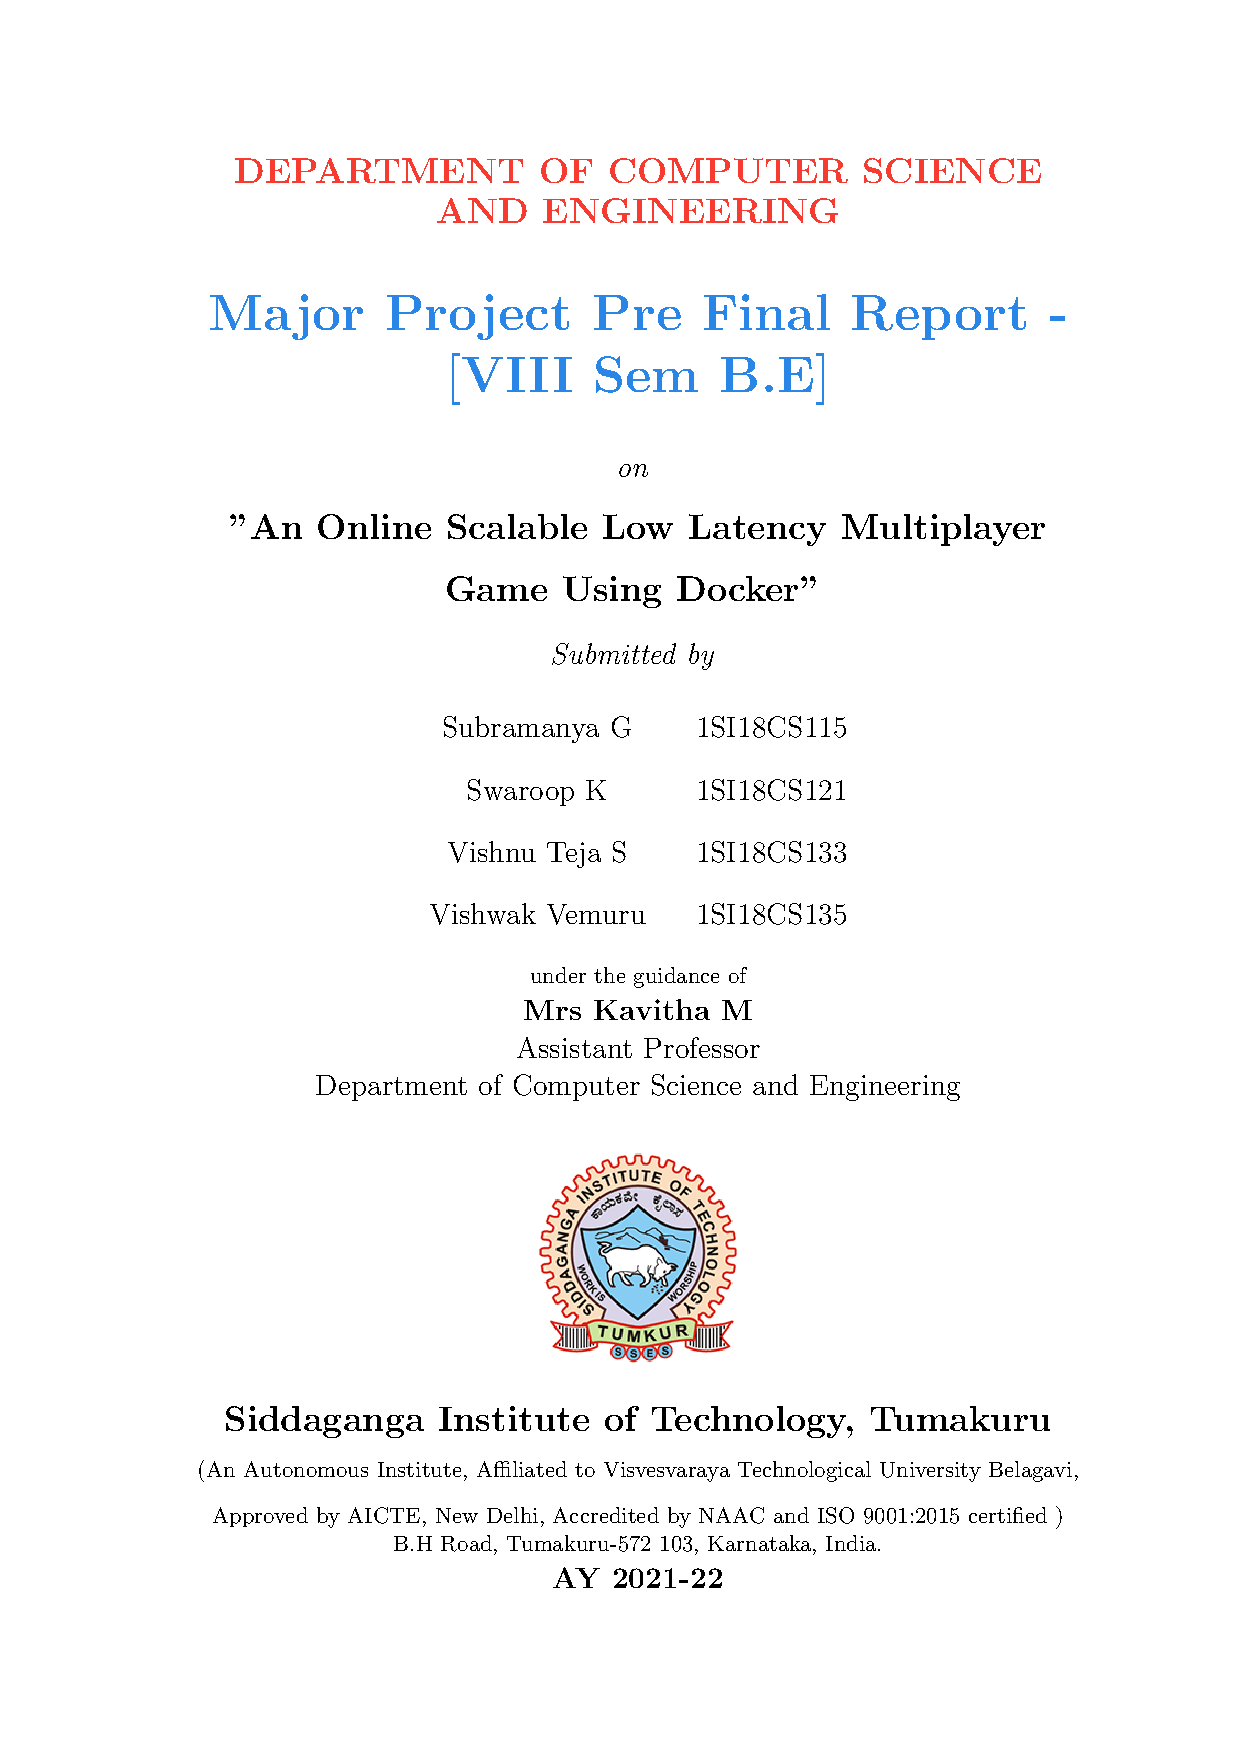
\includepdf[pages=-]{FrontPage.pdf}



\tableofcontents
\thispagestyle{fancy}
\pagebreak
\addcontentsline{toc}{chapter}{Abstract}

%
%\chapter*{}
\section*{Introduction}
\graphicspath{{Introduction/IntroductionFigs/EPS/}{Introduction/IntroductionFigs/}}
The 21st century has been an era of colossal technological advances. Digital literacy is also one of them. It involves digital reading and writing techniques across multiple media forms. So there is an extensive increase in the use of electronic gadgets in this era. As a result, people are prone to various eye diseases. So, detecting them at an early stage is of utmost importance. 
Electroencephalography(EEG) is a test that detects abnormalities in the brain waves or the electrical activity of the brain. An EEG Sensor can be used to detect all those brain waves. Among those detected brain waves, some waves will be associated with the blink action. Those wave frequencies need to be separated and finally, we must calculate the blink frequency. 
Blink frequency helps detect many eye disorders. Detecting an eye disease at a very early stage will help in preventing many adverse effects. Hence, Blink analysis could be a very good contribution to society in detecting various eye diseases.
\section*{Objectives}
\begin{enumerate}
\item To find a suitable sensor and compatible device to detect the eye blinks
\item Collection of blink data required for blink analysis and making sure the data collected will be from both healthy patients and ones who are diagnosed with eye diseases.
\item To analyze the data collected from the selected device and extract blink-related information in real-time.
\item To display results obtained from blink analysis.
\end{enumerate}

% ----------------------------------------------------------------------

%\section*{Literature Survey}
The phenomenon of blink is at an unusual crossroad of a variety of scientific and medical disciplines, as it provides information on ocular surface health, on the cognitive state, on psychological health and disease, and on alertness and fatigue. Precisely for this reason, the blink process is difficult to study: with local and far-reaching, endogenous and exogenous input, the output is seldom driven by one overriding force.

	A blink can be defined as a lid closure of varying speed, frequency, force, and duration. The normal blink rate is about 12 blinks/minute, and the variability among individuals and with the task is widely recognized.\cite{9302890}[1]
\bibliographystyle{ieeetr}
\bibliography{citation}.The below table shows the different factors that affect the blink.
\begin{figure}[h]
    \centering
    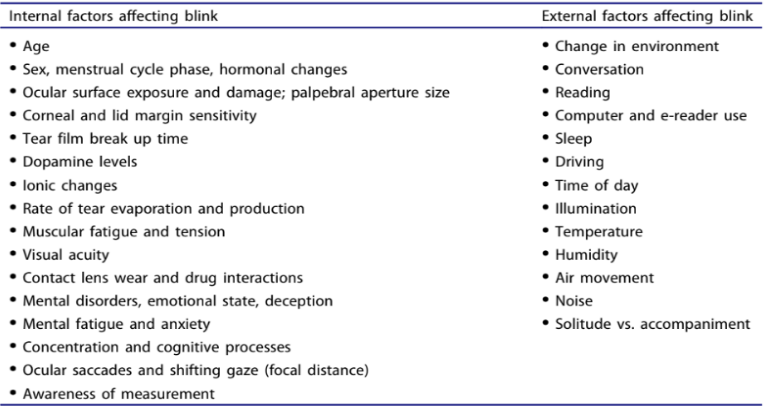
\includegraphics[height=6.5cm]{images/factors.png}
\end{figure}	
	
Our main focus is to detect eye blinks and there are various methods for the same. The two Major methods are as follows:
\begin{enumerate}
\item \textbf{Image processing: }
Image processing is a method to perform some operations on an image, to get an enhanced image, or to extract some useful information from it. It is a type of signal processing in which input is an image and output may be an image or characteristics/features associated with that image. In the paper[2], a web camera is used. Using the Viola-Jones technique face is being detected and after that eyes are detected using the thumb rule. From eyes, eye blinking was determined by converting the eyes template in binary form, which is used afterward for application.
\item \textbf{Wearable Sensors: }
\begin{itemize}
\item \textbf{Electrooculography (EOG)} - Blinks are measured with the EOG when the electrodes are placed vertically above the eyebrow and on the malar prominence in line with the pupil and it is defined as minimal voltage change during a certain period of time.[3]
\item \textbf{Electromyography (EMG)} is habitually used in blinking research to register the relationship between the orbicularis oculi muscle (OOM) and levator palpebrae superioris muscle (LPS).EMG is usually coupled to another system, such as a magnetic search coil or EOG that allows the registration of eyelid positional changes. The simultaneous use of EMG and EOG may be particularly useful for recording eyelid position OOM activity in situations where fixation of the head is not possible.[4]
\item \textbf{Infrared} reflectance utilizes an infrared (IR) LED to illuminate the eye surface and another device, such as a phototransistor or a photodiode, that detects IR light reflected back from the eye. The blink signal is analyzed based on the difference between the light emitted and the light reflected from eyelid and eyeball and is processed by a microcomputer equipped with an analog-to-digital (AD) converter.[5]
\item \textbf{Electroencephalography (EEG)} is at the core of brainwave technology. In EEG it monitors and records the brain activities with the use of electrodes that are attached to a persons’ head. Brains’ neurons emit electrical impulses to communicate with the rest of our bodies which are recorded by electrodes. In the past few years, there’s a rapid advancement and improvement which led to the development of more affordable EEG. This opened limitless possibilities in brainwave technology.[6]
\end{itemize}
\end{enumerate}

After going through all the possible methods, we finally choose to use an EEG device for this project. Because, these are non-invasive, portable, and less expensive than other devices.


\section*{Motivation}
\begin{itemize}
\item The pandemic has increased our dependence on screens for activities that could otherwise have been done offline.A new study and survey  released by NortonLifeLock, examining consumers’ at-home online behaviours, show that two in three Indians surveyed (66\%) have become addicted to being online as a result of the pandemic.The amount of time they spent on screens, aside from educational or work purposes, has increased significantly during the Covid-19 pandemic.Exposure to gadgets can have long term effects specifically when it comes to eyes.Hence using blink analysis it's possible to detect disease related to eyes at an early stage and treat it well.
\item Building an application using a wearable device to detect eye blinks which can help detect various eye-related diseases.
\item Real time analysis -  Analyzing a patient's blink data in real-time helps to identify the abnormalities in the blink rate or parameters related to blinking can help the patient get diagnosed early.
\end{itemize}

\section*{Methodology}
\begin{figure}[h]
    \centering
    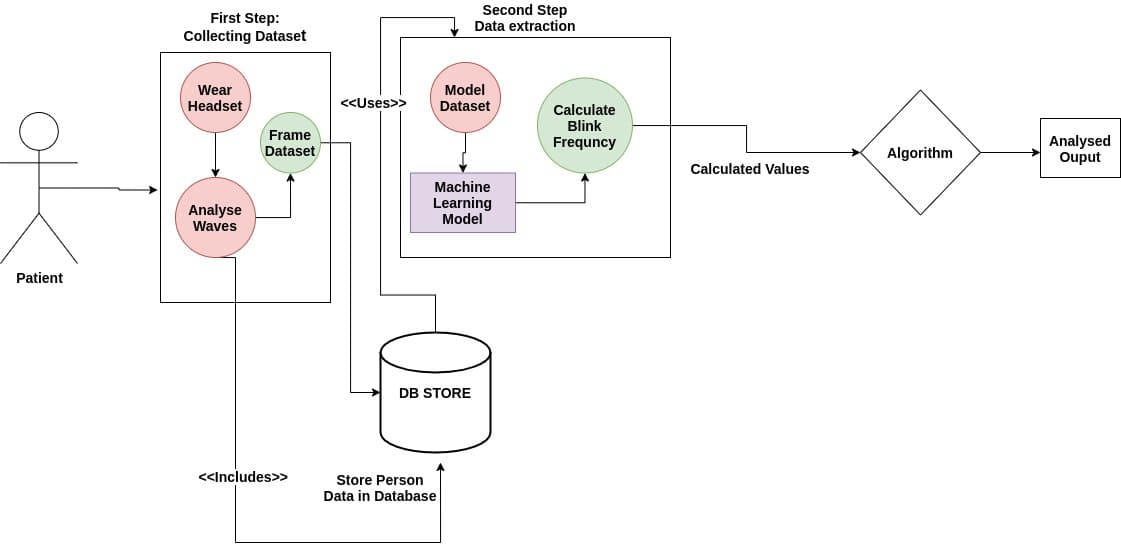
\includegraphics[height=7.5cm]{images/uml.jpg}
\end{figure}

%\textbf{Algorithm used to detect eye blinks :} EEG peak detection algorithm and ML algorithms.
\section*{Tools and Technologies}
\begin{enumerate}
\item Brainsense EEG Sensor
\begin{itemize}
\item Raw EEG at 512Hz
\item Operating voltage 2.97-3.63V
\item Frequency range - 3-100Hz
\end{itemize}
\item NeuroView Software - associated with the sensor device
\item MatLab Software for signal processing and its analysis
\item Jupyter Notebook
\item React, Flutter - for Frontend of application 
\item Django, Node JS - for backend application

\end{enumerate}
\section*{Expected Outcomes}
\begin{enumerate}
\item Results obtained from the Effective and efficient analysis of the real-time data
\item Applying the obtained results in the finding of abnormalities in eye blinks.
\end{enumerate}
\section*{Conclusion}
Using this portable and non-invasive EEG device, the user could get information about any abnormalities in eye blinks from our application. This work is an initial step in the detection of eye abnormalities using sensors with real-time data.


%\bibliographystyle{plain}
%\cleardoublepage
%\addcontentsline{toc}{chapter}{Bibliography}
%\bibliography{References/references}

\section*{Abstract}
%	\paragraph{\normalfont{In this project we wish to develop an Online Scalable Low Latency Multiplayer Game Using Docker. An online multiplayer game allows users from across the world to connect and play together. Most modern multiplayer games use the client-server architecture. However, in these types of online games, there are issues of latency and performance. We propose to solve these issues using Docker containers. Docker containers can be deployed on a cloud nearest to the client reducing latency and they also enable easy management of game servers. }}
	
	
	\paragraph{\normalfont{An online multiplayer game allows users from across the world to connect and play together. Most modern multiplayer games use the client-server architecture. However, in these types of online games, there are issues of latency and performance. To solve these issues, we are building an online scalable low latency multiplayer game using Docker containers. Docker containers can be deployed on a cloud nearest to the client reducing latency and they also enable easy management of game servers. }}
	
	\paragraph{\normalfont{The game would be implemented in the form of a web application. The basic architecture consists of the game is a client-server model. Any number of clients can join the server and each client has their own game instance in the server, grouped under rooms. A cluster of docker containers are used to run the server. We make use of the phaser game framework to render the game, maintain the game state and we use MongoDB for the database. The Docker containers will be hosted on a cloud. }}
	
	\paragraph{\normalfont{The game will be able to provide cross-platform support. The game would be a fast-paced combat game and will be able to establish real time communication between the user’s browser and a server. The game will also be able to allow users to create private and public rooms for game sessions and the game server will run on docker containers. }}
	
\chapter{Introduction}
	\thispagestyle{fancy}
	\paragraph{\normalfont{A multiplayer game is a game in which more than one person can play in the same game environment at the same time, either locally and on the same computing system, locally and on different computing systems via a local area network, or via a wide area network, most commonly the Internet.}}
	
	\paragraph{\normalfont{The game will be having the following features:}}
	\begin{itemize}
		\item Orthogonal Top-down view
		\item Co-op Combat
		\item Character Customization
		\item Public and private rooms for game sessions
	\end{itemize}
	\paragraph{\normalfont{There are two types of multiplayer games:}}
	\begin{enumerate}
		\item Non-networked Games: These are predominantly 2-player games played on a single device with multiple controllers.
		\item Networked Games: These allow users from different devices to connect to each other and play the games. It has following two categories: 
		\begin{enumerate}[a.]
			\item Local Multiplayer: They are always played on the same local network.
			\item Online Multiplayer: They Can be played through any device across the Internet.
		\end{enumerate}
	\end{enumerate}
	
	\paragraph{\normalfont{The game would be an online multiplayer game where players are not restricted to the same network. There are two ways of implementing this:}}
	\begin{enumerate}
		\item Peer-to-Peer: In these types of games, one of the players become the authority and all other players has to send the data to the authoritative person. The authority updates the game states and sends the updated states to all the other players. Peer-to-Peer type of game has the following disadvantages:
		\begin{itemize}
			\item The peer who becomes the authority has to have a large bandwidth.
			\item If the authoritative peer exits, the game automatically ends for all players. 
			\item Peer server can change the states, which affects the playing experience for all players.
		\end{itemize}
		\item Client Server: In these types of games, a dedicated server is set up. All clients must connect to this server and the server is the authority. This successfully overcomes all the disadvantages of the Peer-to-Peer types of online multiplayer games. 
	\end{enumerate}
	
	\paragraph{\normalfont{Most modern multiplayer games use the client-server architecture. However, in these types of online games, there are issues of latency and performance.  The primary causes of latency are and other performance issues are:}}
	\begin{itemize}
		\item Bandwidth: Online multiplayer games generally requires a high bandwidth.
		\item Wired connections have low latency than Wireless connections. 
		\item Internet network hardware.
		\item Remote server locations and connections used by remote server.
		\item Internet service provider. 
		\item Network Interference. 
	\end{itemize}
	
	\paragraph{\normalfont{The solution to the above problems is to use docker containers. Docker is an open platform for developing, shipping, and running applications. Docker enables us to separate our applications from our infrastructure so we can deliver software quickly. Docker provides the ability to package and run an application in a loosely isolated environment called a container. The isolation and security allow us to run many containers simultaneously on a given host. Containers are lightweight and contain everything needed to run an application, so we do not have to rely on what is currently installed on the host. }}
	
	\paragraph{\normalfont{Docker provides tooling and a platform to manage the lifecycle of containers: }}
	\begin{itemize}
		\item Develop applications and its supporting components using containers. 
		\item The container becomes the unit for distributing and testing applications. 
		\item Deploy applications into a production environment, as a container or an orchestrated service. This works the same whether the production environment is a local data center, a cloud provider, or a hybrid of the two.
	\end{itemize}

	\paragraph{\normalfont{In the case of online multiplayer game, docker enables easy management of game servers and allows for deployment on the cloud. This allows an instance of the game to run on the nearest cloud server to the user solving the issues of latency. As there are multiple docker containers running the server, the performance is boosted. Further, using docker containers enables support for rolling deployment, autoscaling, monitoring and maintenance of the game server.}}
	
	\chapter{Literature Survey}
	\thispagestyle{fancy}
	
	\paragraph{\normalfont{Many works and papers were referred and the following things were noted.}}
	
	
	\paragraph{\normalfont{Cloud gaming is the future for the gaming industry and it allows users to play games anywhere, anytime and from any device. The paper \cite{paper1} addresses the main challenges in the cloud gaming namely, resource allocation and ensuring quality of user experience. \cite{paper1} also elaborates on how to improve the performance of cloud gaming by initializing the cloud gaming package inside Docker containers which will allow the application to be more reliable by secularizing its resource allocation and increasing the overall performance of the cloud gaming system and makes it more reliable while utilizing less resources.}}
	
	\paragraph{\normalfont{The real-time strategy game StartCraft: Brood War is a commonly used domain for AI research, with a pre-installed collection of AI development tools supporting all the major types of StarCraft bots. \cite{paper2} presents a dockerized version of StarCraft. The implementation in \cite{paper2} provides a convenient way to deploy StarCraft AIs on numerous hosts at once and across multiple platforms despite limited OS support of StarCraft. \cite{paper2} also describes the design of the Docker images and presents a few use cases.}}
	
	\paragraph{\normalfont{Mobile Edge Computing (MEC) is an emerging network paradigm that provides cloud and IT services at the point of access of the network. Such proximity to the end user translates into ultra-low latency and high bandwidth, while, at the same time, it alleviates traffic congestion in the network core. Due to the need to run servers on edge nodes, key element of MEC architectures is to ensure server portability and low overhead. \cite{paper3} proposes a tool that can be used for this purpose - Docker. Docker is a framework that allows easy, fast deployment of Linux containers. \cite{paper3} focusses on the suitability of Docker in MEC scenarios by quantifying the CPU consumed by Docker when running two different containerized services: multiplayer gaming and video streaming. The results of tests performed by the authors in \cite{paper3}, with varying numbers of clients and servers, yield different results for the two case studies: for the gaming service, the overhead logged by Docker increases only with the number of servers; conversely, for the video streaming case, the overhead is not affected by the number of either clients or servers.}}
	
	\paragraph{\normalfont{The recent developments in the field of cloud computing allow cloud gaming to provide high-end quality of experience to the users. \cite{paper4} claims that the fundamental requirement of gaming is to provide maximum quality of gamer experience, however cloud gaming suffers in terms of providing Quality of Experience, because the network transmission of game scenes from cloud game server to gamer device is distant. The author endeavours to minimize latency and increase performance in cloud gaming through this paper. \cite{paper4} proposes moving the cloud game server to the fog nodes present at the edge network of the player based on Node selection algorithm. \cite{paper4} also suggests that, to increase the performance of cloud gaming, traditional virtual machine should be replaced by light-weight containers.}}
	
	\paragraph{\normalfont{HTML5 has provided many developers the opportunity to experiment with the new possibilities for web development. The authors’ aim, through \cite{paper5} is to give an overview of what this means to the game development community. \cite{paper5} evaluates new HTML5 elements and JavaScript features. It also highlights WebGL, Canvas and WebSockets that have given developers the opportunity to flaunt their creativity by manipulating images, creating 3D environments and providing real-time interaction.}}
	
	\paragraph{\normalfont{Big Two is an online multiplayer game with imperfect information. In this game, each player plays without knowing the opponent's confidential information. \cite{paper6} considers Big Two as an example in elaborating the need for web-based multiplayer games with imperfect information to have real-time communication for handling rapid information changes and the condition of the game state at any time. \cite{paper6} proposes a new framework for web-based multiplayer games with imperfect information. \cite{paper6} utilizes an open-source WebSocket, namely Socket.IO, and implements this framework in Big Two as a case study.}}
	
\chapter{Problem Statement and Objectives}
	\thispagestyle{fancy}
	\textbf{Problem Statement: }
	To develop an Online Scalable Low Latency Multiplayer Game Using Docker
	\newline
	\newline
	\newline
	\textbf{Objectives:}
	\newline
	\begin{itemize}
		\item To enable cross-platform support by building a web application.
		\item To build a fast-paced combat game.
		\item To establish real time two-way interactive communication session between the user's browser and a server.
		\item To enable users to create private and public rooms for game sessions.
		\item To containerize the game server and reduce the game server overhead.
		
	\end{itemize}
	
\chapter{Project Design}
	\thispagestyle{fancy}
	\paragraph{\normalfont{The Fig. \ref{fig:archi} shows the architecture of the game. The top part of the architecture diagram depicts the server. Any number of clients can join the server and each client has their own game instance in the server, grouped under rooms. A cluster of docker containers are used to run the server. We also make use of phaser game framework and MongoDB for the database. We make use of Google Cloud VM instance for the hosting of our game.}}
	\begin{figure}[ht!]
		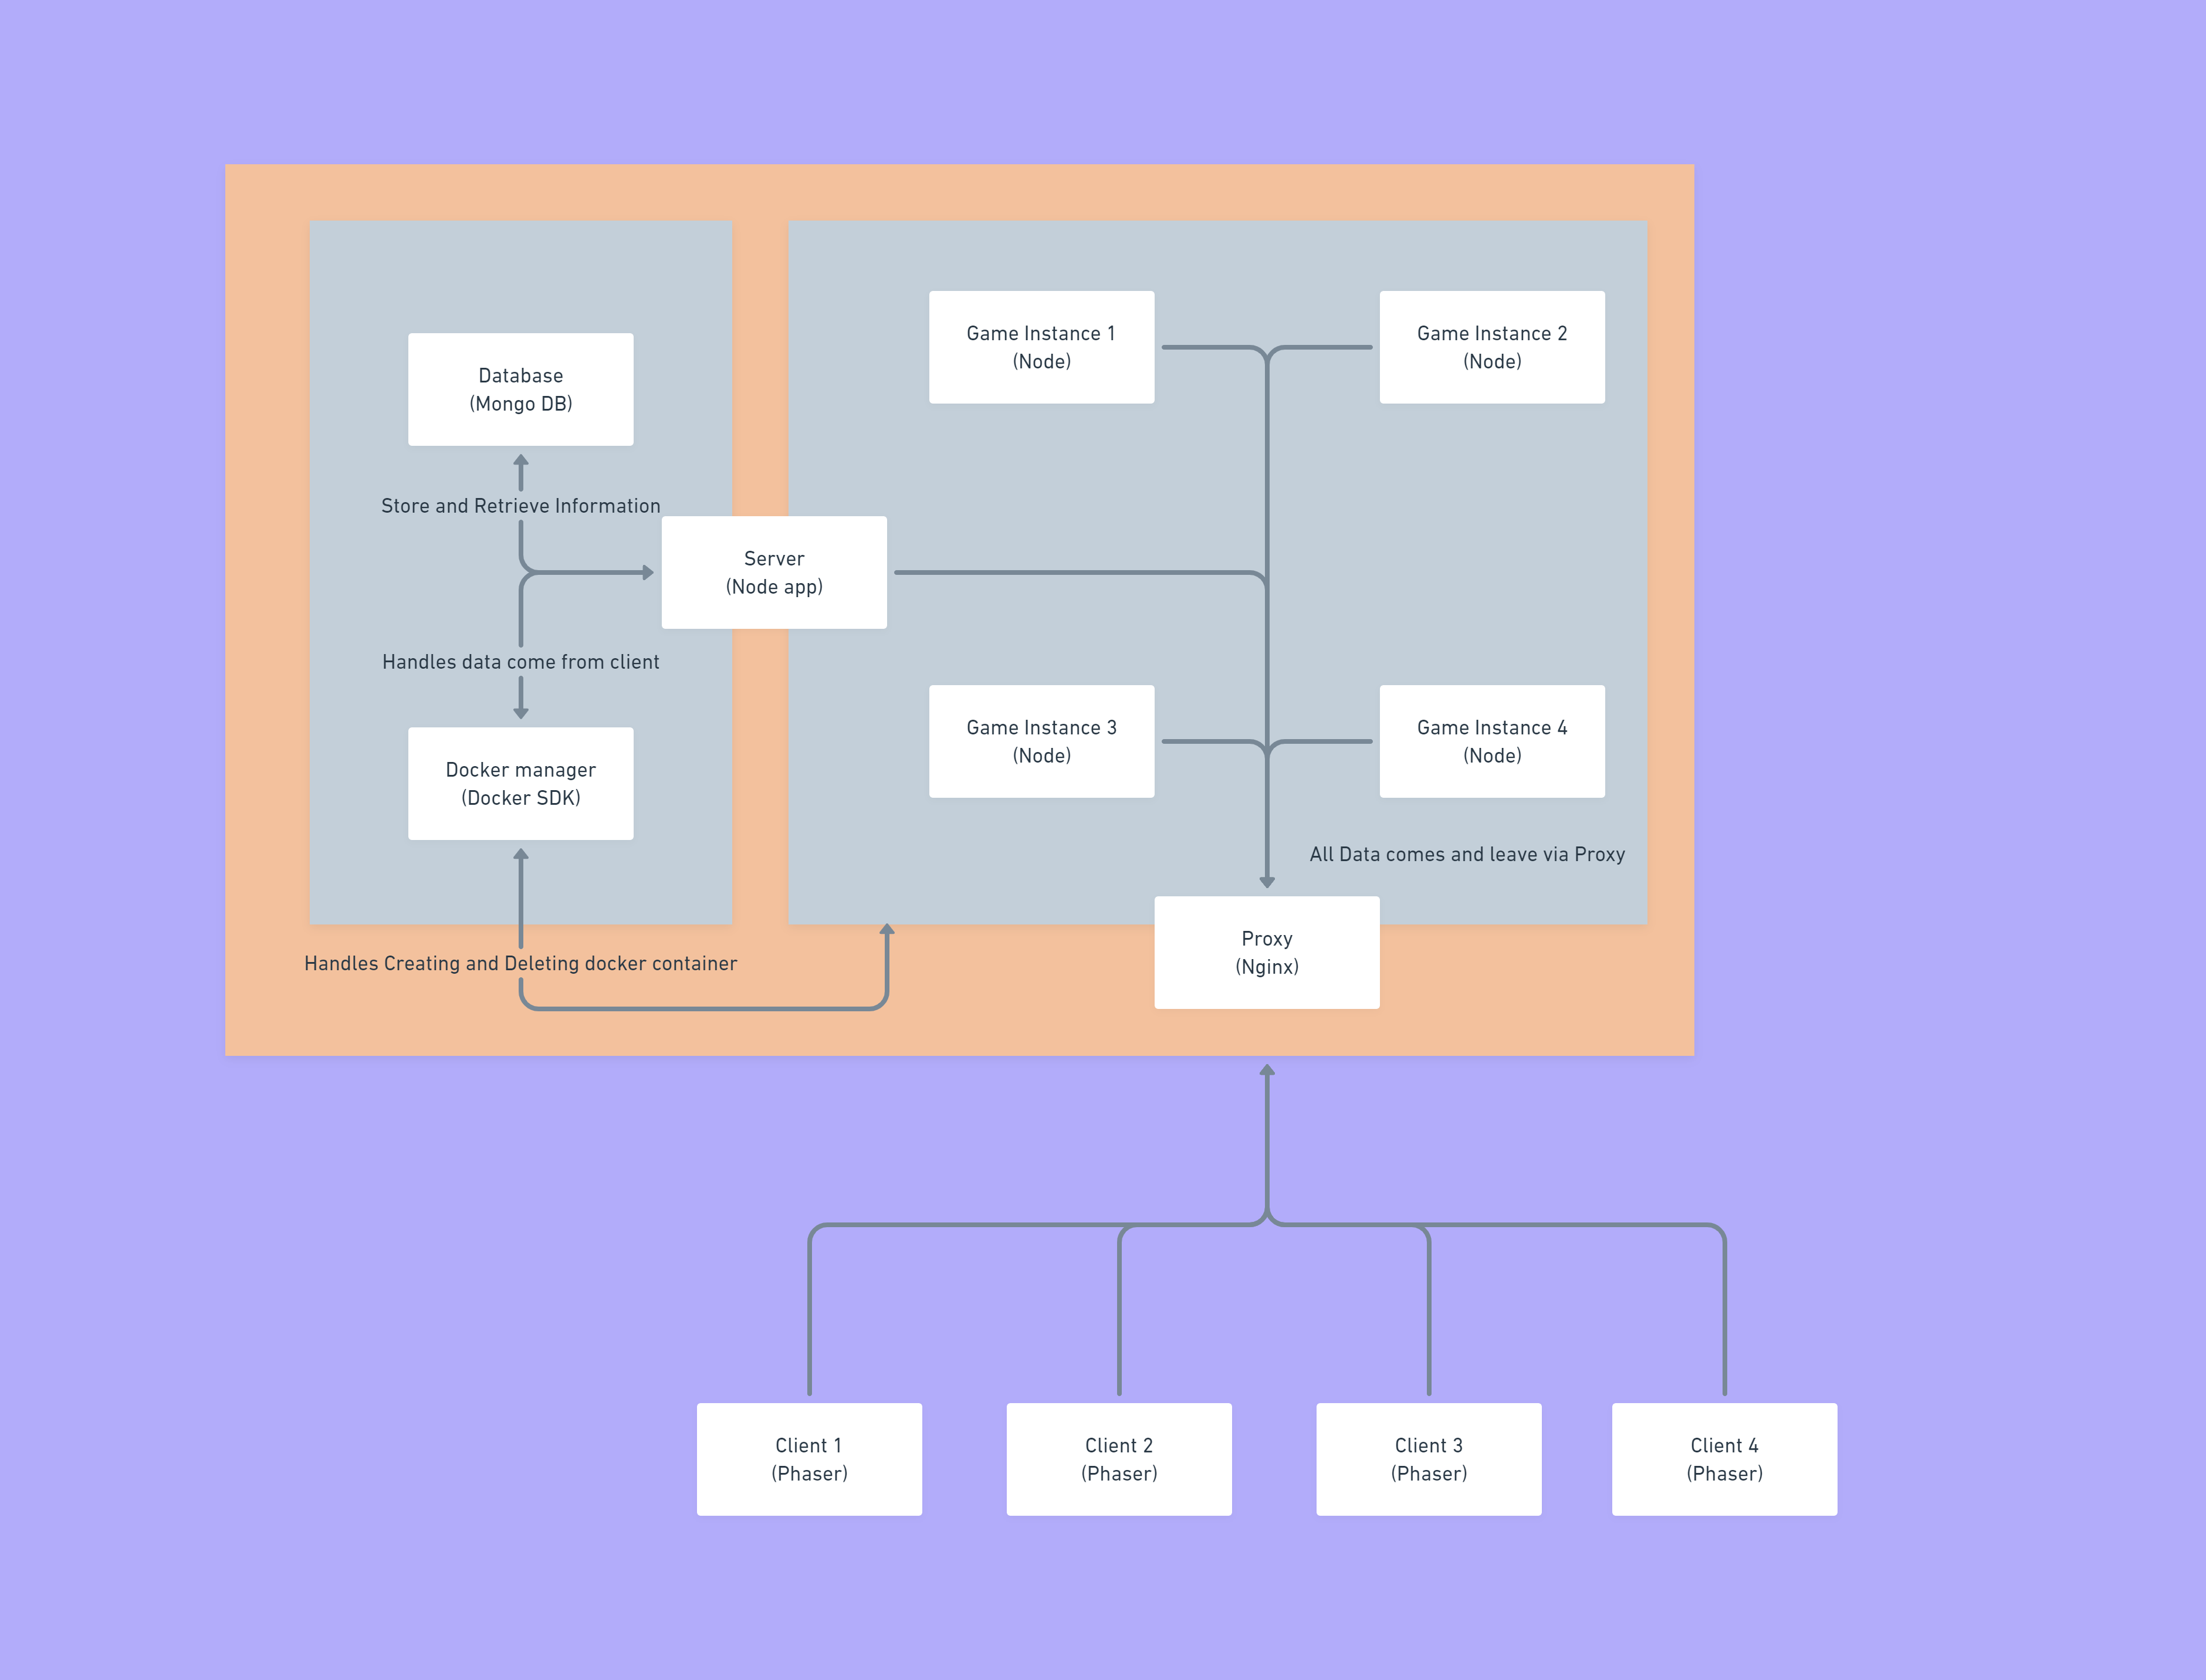
\includegraphics[scale=0.1]{archi.png}
		\centering
		\caption{An overview of the basic game architecture}
		\label{fig:archi}
	\end{figure}
	
	\paragraph{\normalfont{The following are the major components of the architecture: }}
	\begin{enumerate}
		\item \textbf{Database:} In this project we make use of MongoDB database. MongoDB is a cross-platform database, classified as a NoSQL database. It uses JSON like documents with optional schema. We use this database primarily to store the state of the game. We store the state for each room (A room represents a group of users playing together) which a group of users connect to. We store the room ID, the members of the room, their characters and respective inventory ie., the weapons, coins collected etc. 
		
		\item \textbf{Docker Manager:} Docker is a set of platform-as-a-service products that use OS-level virtualization to deliver software in packages called containers. Docker manager is a tool that runs the docker SDK. It helps us to create and manage the various rooms in the game. Each docker instance will run a single instance of the game. The database and the docker manager constitute the backend of our application. 
		
		\item \textbf{Server:} The server uses Node.js to connect to the docker containers running the game to the users. Node.js is an open-source, cross-platform backend JavaScript runtime environment that runs on the V8 engine and executes the JavaScript code outside the web browser. It acts as a middleware between backend and frontend. It provides a layer of abstraction between the database and docker manager. It also manages the user authentication. 
		
		\item \textbf{Game Instance:} It is a docker container that is created and managed by the docker manager. It acts as the frontend. Each game instance runs a game server within a docker container which the players can join. It manages the users who have joined, broadcasts the game state to all the users and creates the maps of the game procedurally. 
		
		\item \textbf{Proxy(Nginx)}: Each user connecting to the application must connect to the containers through different ports. But, the number of ports available ports is limited - there are 65535 ports out of which 2000 are meant for special purposes. As a result of which we need something that maps each container to the outside world. The advantage of using docker is that, a user can connect to a docker instance or container using its name. So we use a proxy that maps the external request of the user to the internal network. In our application, the proxy works by mapping a request with subdomain having the name of a docker instance to that particular docker instance. For example, \emph{abc.domain.com} connects to the \emph{abc} container. 
		
		\item \textbf{Client:} The client program uses the Phaser game engine and it runs on the browser of the user. The specifics of the game are written in TypeScript files. The client obtains the data from the game instance and renders it in the web browser for the user. Any action made by the user, constitutes a change in the state of the game, will be sent to the game instance which is then broadcasted to the room that the game instance is part of. 	
	\end{enumerate}
	
	\begin{figure}[ht!]
		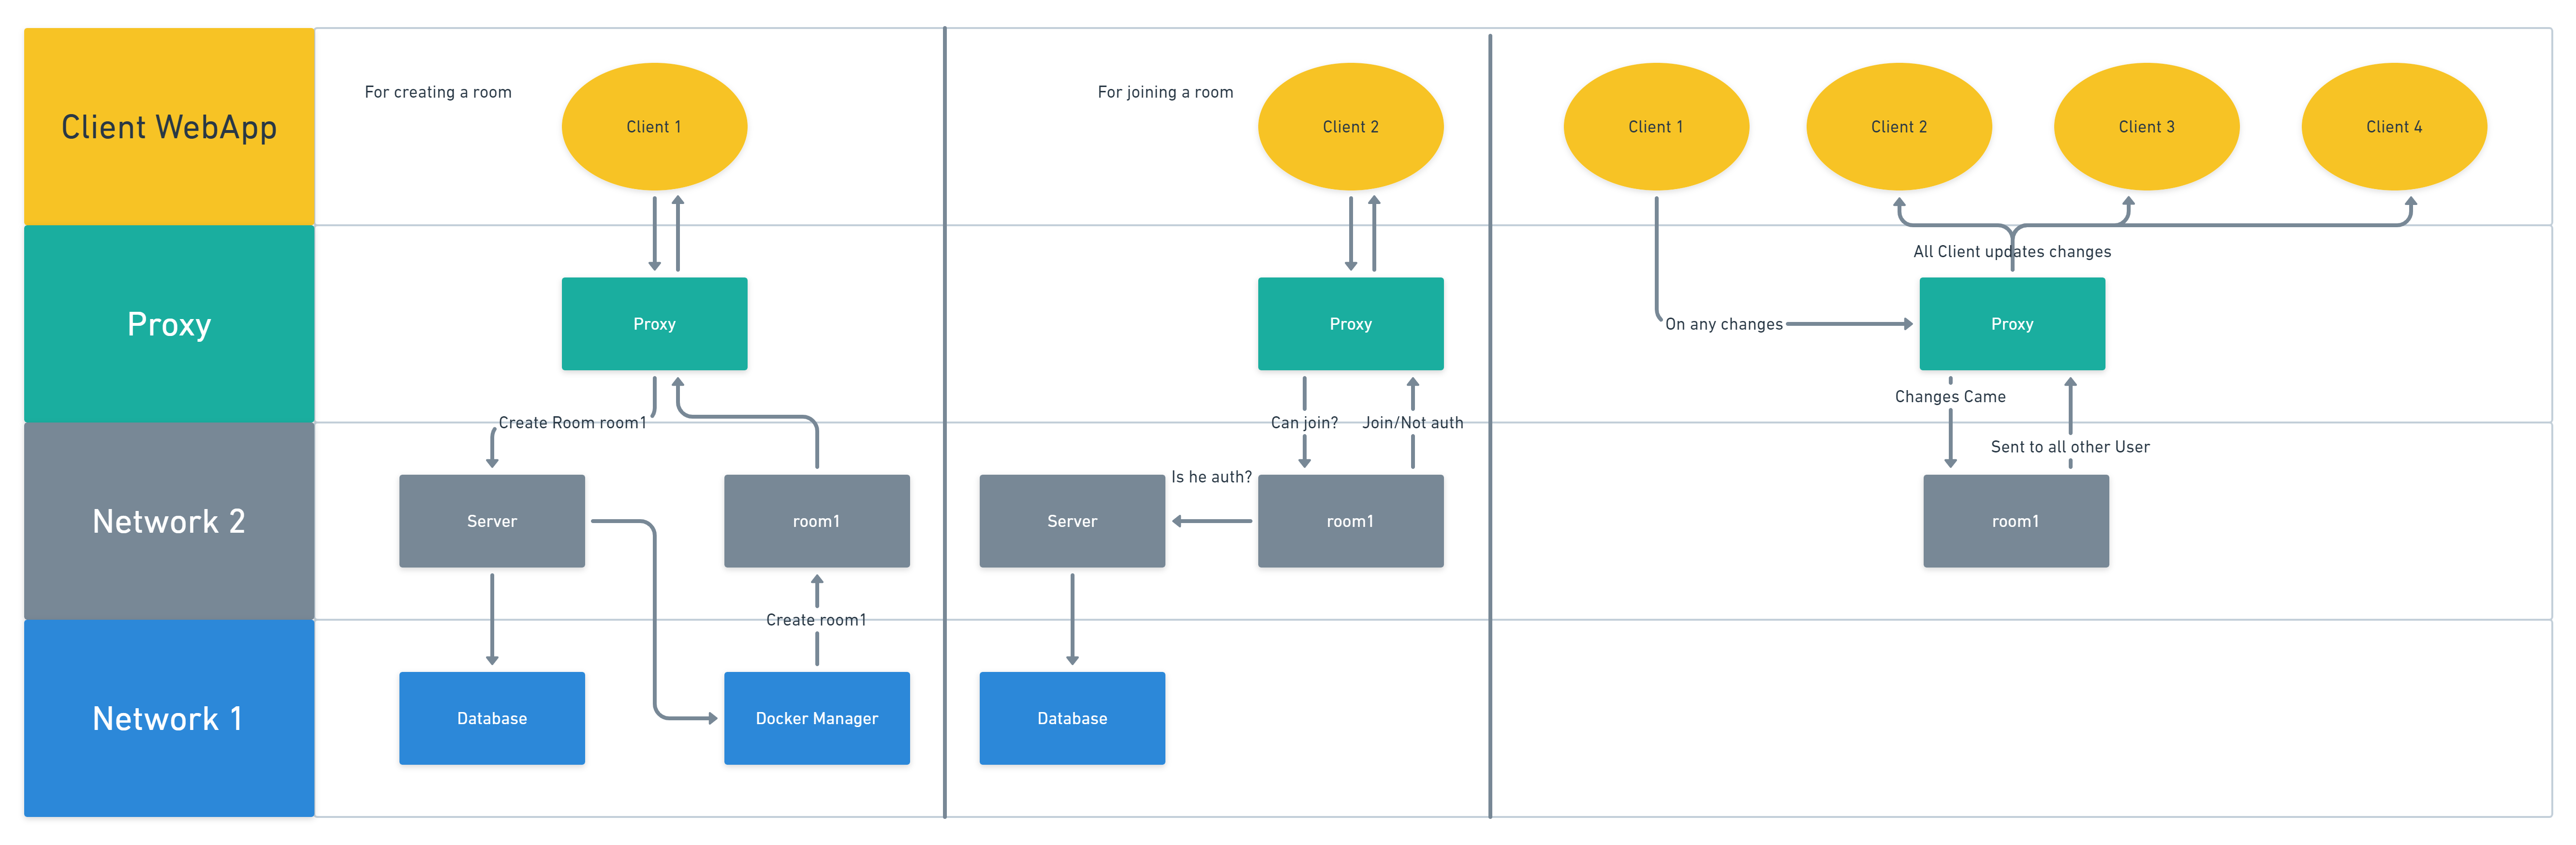
\includegraphics[scale=0.09]{swimlane.png}
		\caption{Swimlane diagram depicting the basic use cases of the application}
		\label{fig:swim}
	\end{figure}

	\paragraph{\normalfont{The Fig. \ref{fig:swim} shows the flow of the actions required for some basic use cases of the application. These are briefly described as follows: }}
	\begin{itemize}
		\item \textbf{Creating a room: }A room is created when a new game session is to be started. One of the users sends a request via the proxy to the server. The server then requests the docker manager to create a container for the room and also stores the necessary information in the database. After successful creation of a docker container (game instance container), the user will be notified. The other users can join this room by using the ID. It should be noted here that the initial user joins through the proxy and it is mapped to the created game instance container. 
		
		\item \textbf{Joining a room: }A user who wishes to join a room sends a request to the room via the proxy using the room ID. The room verifies the credentials of the user from the server (The server checks the credentials in the database). After the successful authentication, the user will be allowed to join the room.
		
		\item \textbf{Normal game play: }The group of users in a room are playing on the same game instance, any change in the state of the game made by one user must be synchronised to all the other users. Thus, every change results in the client sending its state to the game instance, which will then be broadcasted to all the users. We make use of socket.io to enable broadcasting without explicit querying from the client.
		
	\end{itemize}	

\chapter{Software and Hardware Requirements}
	\thispagestyle{fancy}
	\paragraph{\normalfont{\textbf{Software Requirements \newline}Server Side:}}
	\begin{itemize}
		\item Docker – For containerization
		\item Docker Manager – For managing the container
		\item Node – For server scripting
		\item Express – For server web application framework
		\item Socket.io – For handling the WebSocket
		\item Nginx – For reverse proxy
		\item MongoDB – Database
	\end{itemize}
	\paragraph{\normalfont{Client Side:}}
	\begin{itemize}
		\item TypeScript - Add static typing to the language
		\item Phaser – Game engine
	\end{itemize}
	
	\paragraph{\normalfont{Development: }}
	\begin{itemize}
		\item Docker desktop
		\item VS Code
	\end{itemize}
	\paragraph{\normalfont{\textbf{Hardware Requirements \newline}As the game is implemented in the form of a web app, any hardware configuration which can run a web browser can effectively run our game. However,  a good network connectivity is required. }}
	
	
	
\chapter{Project Plan and Cost Estimation}
	\thispagestyle{fancy}
	\begin{figure}[ht!]
		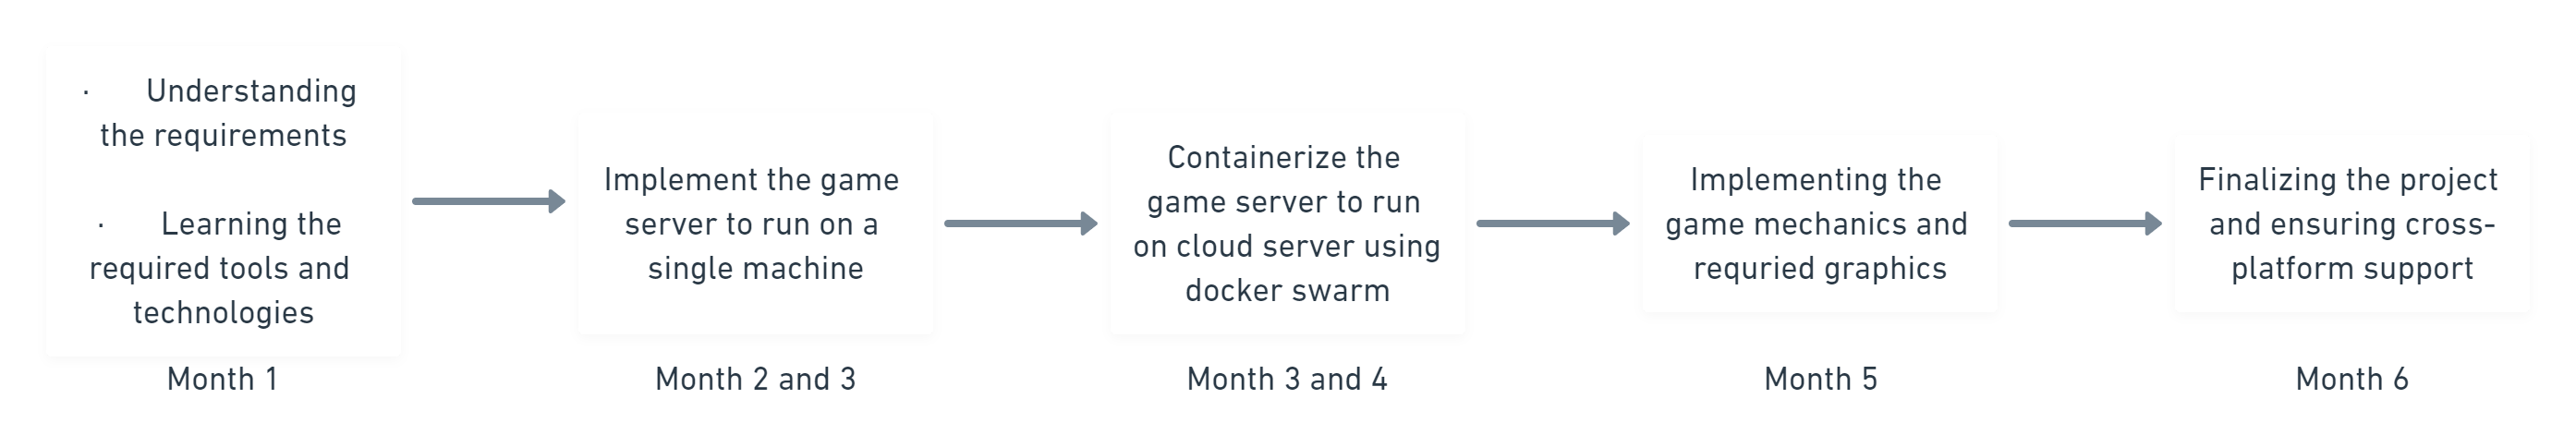
\includegraphics[width=\linewidth]{plan.png}
		\centering
		\caption{An overview of the project plan}
		\label{fig:plan}
	\end{figure}
	
	\paragraph{\LARGE{Project planning}}
	\paragraph{\normalfont{The Fig. \ref{fig:plan} shows an overview of the plan for implementing the project. We have divided the implementation of the entire project into five phases spanning across six months. The tasks planned in these months are breifly described as follows: }}
	\begin{itemize}
		\item \textbf{Month 1: }Understanding the requirements: 
		The key to successful software development is that all developers develop a clear and uniform understanding of the application requirements. To understand the requirements, we considered making a web application for the game. We planned on the basic architecture of the game decided on some tools and technologies needed to build the project. \newline
		Learning the required tools and technologies: The following are the tools that we have decided for the implementation of the project. 
		\begin{itemize}
			\item Docker Swarm
			\item Docker Manager
			\item Phaser
			\item TypeScript
			\item Nginx
		\end{itemize}
		We will learn these technologies over the course of the project with the help of tutorials, courses and relevant documentations. 
		
		\item \textbf{Month 2 and 3: }Implementing the game server to run on a single machine: 
		We begin the implementation of the game by making the game server run in the local environment. We will make use of some placeholder assets for the game, while testing the game server. The game server would be running on a single machine and multiple users will be able to connect to it. We will make use of 2D Phaser game engine to render the generated level using the placeholder assets and the game engine would also be able to handle the collision and overlap events. We will make use of Drunkard Walk algorithm for procedural generation of levels. We will make use of Socket.io package to handle bi-directional communication between the server and the user.
		
		
		\item \textbf{Month 3 and 4: }Containerize the game server to run on cloud server using docker swarm: 
		Docker swarm is a container orchestration tool, meaning that it allows us to manage multiple containers deployed across multiple host machines. In this step of implementation, we containerize the game server, so that it can run in docker containers. We will have to make docker images for the various components of the game such as game server, docker manager and database. We will make use of Nginx for the purpose of reverse proxy. We will then be able to deploy it in the local docker swarm called as stack.
		
		\item \textbf{Month 5: }Implementing the game mechanics and required graphics
		In the this step of implementation, we plan to implement the specifics of the game which are: 
		\begin{itemize}
			\item Core game mechanics
			\item Various types of enemies
			\item Character skins
			\item Weapons
			\item Other game assets
			\item Level progression
			\item In-game economy
		\end{itemize}
		
		\item \textbf{Month 6: }Finalizing the project and ensuring the cross-platform support: 
		We will finalize the project, by packaging the client, server, game server and the docker manager. We will try to optimize the docker containers to improve the performance of the game. We will implement platform specific controls such as touch screen for android, controllers for consoles and so on. We will then be able to deploy the final project to the google console platform.
		
			
	\end{itemize}
	
	\paragraph{\LARGE{Cost Estimation}}

	\begin{center}
		\begin{tabular}{ | c | m{2.5cm} | m{7cm} | c | }
			\hline 
			\textbf{Sl. No.} & \textbf{Particulars} & \textbf{Description} & \textbf{Approx. Cost} \\
			\hline \hline
			1 & Google Cloud & For hosting the Docker containers & Rs. 5000 p.m \\
			\hline
			2 & Google Cloud Registry & To save and manage the Docker images & Rs. 1000 p.m \\
			\hline
			3 & Software \newline Licenses & Licenses for various proprietary tools we may need to use during the project development & Rs. 5000 \\
			\hline
			4 & Game Assets & Various assets required for the game like background music, player skins, weapons etc. & Rs. 3000 \\
			\hline
			5 & Courses & Courses required for learning the tools and technologies & Rs. 3000 \\
			\hline
			6 & Miscellaneous & Costs for preparing project reports and for stationary requirements & Rs. 5000 \\
			\hline
		\end{tabular}
	\end{center}
	
\chapter{Modules Implemented and Results}
	\thispagestyle{fancy}
	\paragraph{\normalfont{The following images (Fig. \ref{fig:direc}) shows the directory structure of the module implemented: \newline}}
	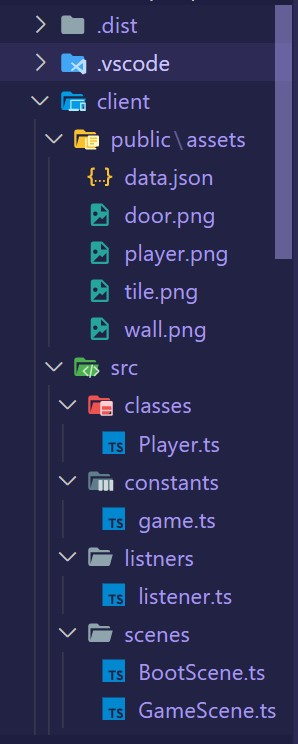
\includegraphics[scale=0.6]{d1.jpg}
	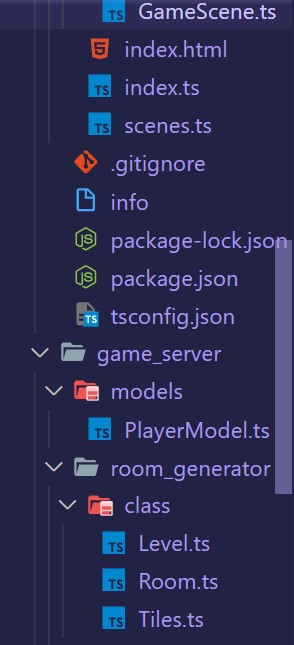
\includegraphics[scale=0.68]{d2.jpg}
	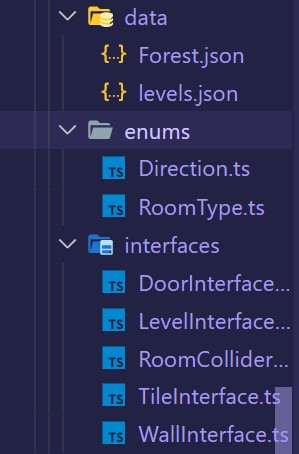
\includegraphics[scale=0.69]{d3.jpg}
	\begin{figure}[ht!]
		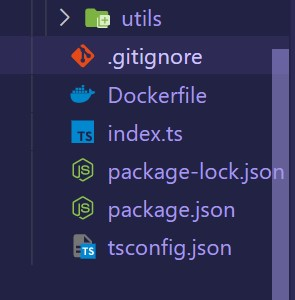
\includegraphics[scale=0.7]{d4.jpg}
		\centering
		\caption{The directory structure of the project}
		\label{fig:direc}
	\end{figure}

	\paragraph{\normalfont{The following parts constitute the implemented module: \newline \textbf{Client Side}}}
	\begin{enumerate}
		\item \textbf{Parcel.js: }We have used the Parcel.js bundler for automatically tracking files and configurations, plugins and dependencies. It allows hot reloading and better diagnostics and also boosts the performance of the application. 
		
		\item \textbf{src/classes/Player.ts: }This file implements the logic required for handling a player in the game. it keeps track of the main player (representing the current user), obtains the inputs from the user and makes the camera follow the main player with smooth animation. 
		
		\item \textbf{src/listners/listener.ts: }This file implements various listeners for the different events that occur in the game. Any module in the application can make use of the listeners implemented in this file. It makes use of sockets to receive events broadcasted by other users and to broadcast events. The following are the listeners implemented so far:
		\begin{enumerate}[i.]
			\item Socket Events: These events are received through the socket from other players. 
			\begin{itemize}
				\item Create Player: This event is triggered when a new user joins a room. After the joining the room, the user must obtain the data of all other users in the room. This is achieved by making use of this event. 
				
				\item Spawn Player: This event is triggered when a new user joins a room. When a new user joins the room, all the other users must be notified and the corresponding player must be created. This is achieved by making use of this event. 
				
				\item Player Movement: This event is used to receive the position and movements off all other players. 
				
				\item Got Map: This event is used to receive the map of a level. 
				
				\item Remove Player: This event is triggered when a user leaves the room. His player is deleted from the game and is broadcasted to all the users. 
				
				\item Level Completed: This event is triggered when a level is completed and a new level is loaded for all the players. 
			\end{itemize}			
			\item Game Events: These events occur by the actions of a user and are broadcasted to all the other users. 
			\begin{itemize}
				\item New Player: This event is triggered when a new user joins a room. His corresponding player is created and this information is broadcasted to all the other players. 
				
				\item Player Movement: This event is triggered whenever a user moves his player. The updated position is broadcasted to all the other players. 
				
				\item Get Map: Requests the server for the map of the level. 
				
				\item Level Complete: This event is triggered when a user completes a level. This information is broadcasted to all the other users and the server is requested to generate a new level. 
			\end{itemize}
		\end{enumerate}
		\item \textbf{src/scenes/BootScene.ts: }This file loads all the required assets for the game. It showws a loading image until loading of all the assets is complete.
		
		\item \textbf{src/scenes/GameScene.ts: }This file renders the current game state to the user. It renders the necessary images, adds colliders and initializes other players. It obtains all the data from the server using listeners and shows it to the user. It uses the listeners from the \emph{listeners.ts} file. 	
	\end{enumerate}
	
	\paragraph{Server Side}
	\begin{enumerate}
		\item \textbf{index.ts: }This file listens for the socket events and broadcasts the data. It creates the procedural maps using room\textunderscore generator. 
		
		\item \textbf{room\textunderscore generator: }It generates a procedural map for a level. It first initializes a 11*11 matrix, and sets the middle of this matrix as the start room. It uses the Drunkard Walk algorithm to populate the rest of the matrix until the maximum number of rooms for all the types of rooms are created.
		Based on that matrix, we create the map with variable width and height. We then generate the walls for each room and the pathway between the rooms as given by the algorithm. We then add the location of the colliders and overlappers. The map converted into JSON format and returned to the server.
		
		\item \textbf{Proxy: }We make of Nginx for the proxy. We have implemented it in a way that \emph{subdomain.domain} request is mapped to the \emph{subdomain} docker container.
		
	\end{enumerate}

	\paragraph{\LARGE{Results:\newline\newline}}
	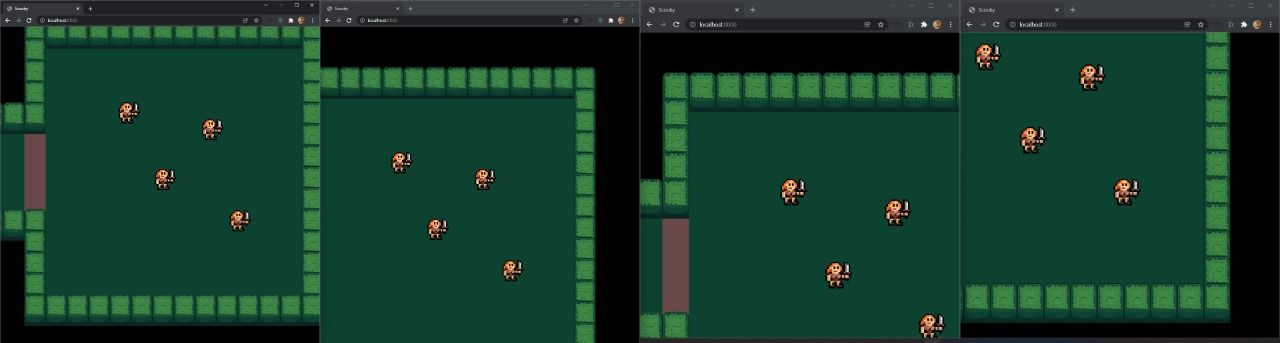
\includegraphics[width=\linewidth]{f1.jpeg}
	\newline
	\newline
	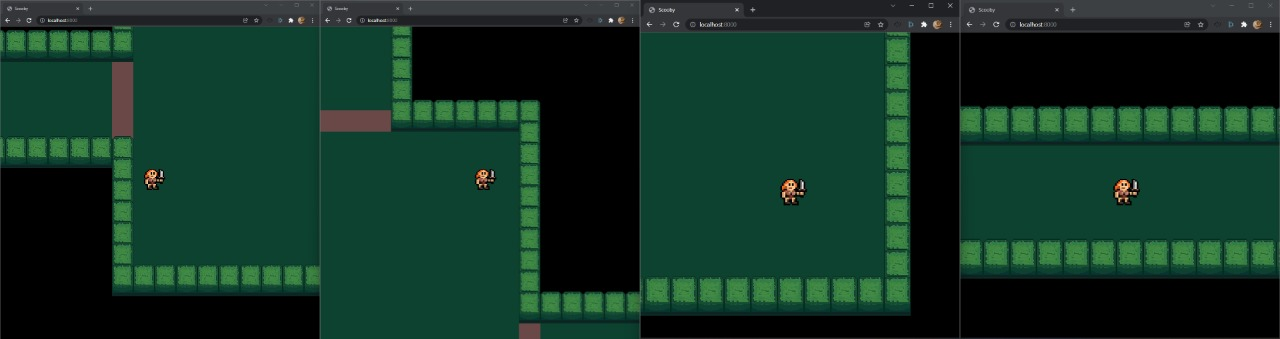
\includegraphics[width=\linewidth]{f2.jpeg}
	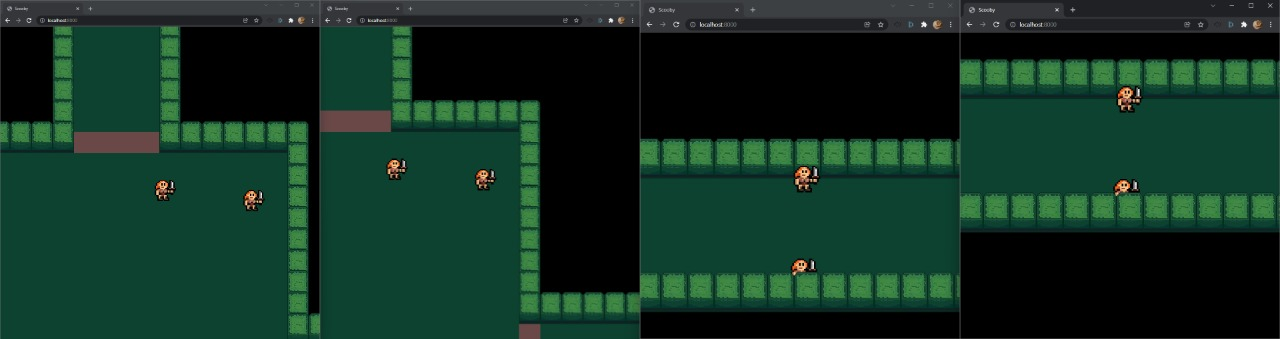
\includegraphics[width=\linewidth]{f3.jpeg}
	\pagebreak
	\pagebreak
	
\addcontentsline{toc}{chapter}{Conclusion}
\chapter*{Conclusion}
	\thispagestyle{fancy}
	\paragraph{\normalfont{The online multiplayer games constitute a significant portion on the gaming industry. With an active userbase of more than two billion players, the industry is worth around thirty thousand crores. Consequently, it is very important for the games to be highly scalable for meeting the evergrowing demands. To enhance user experience, it is crucial for the games to have low latency and feel more responsive.}}
	\paragraph{\normalfont{We use docker containers for the game server which allows us to, easily manage, monitor and maintain the game server, allows for deployment on the cloud, reduces latency by running an instance of the game on the cloud server nearest to the user, boost server performance by using multiple docker containers to run the server, it also enables support for rolling deployment and autoscaling.}}
	\paragraph{\normalfont{We propose to build an online multiplayer game that allow users from across the world to connect and play together. The game would be a 2D multiplayer game that supports features like orthogonal Top-down view, co-op combat, Character customization and public and private rooms for game sessions.}}
	
\section*{}
	\pagebreak
	\addcontentsline{toc}{chapter}{Bibliography}
	\begin{thebibliography}{99}
		\thispagestyle{fancy}
		\bibitem{paper1} Cloud Gaming System in Docker Container Image:\newline \url{http://norma.ncirl.ie/4233/1/arunpugalendhi.pdf}
		
		\bibitem{paper2} Multi-platform Version of StarCraft: Brood War in a Docker Container: Technical Report: \newline \url{https://arxiv.org/pdf/1801.02193}
		
		\bibitem{paper3} Characterizing Docker Overhead in Mobile Edge Computing Scenarios: \newline \url{https://dl.acm.org/doi/pdf/10.1145/3094405.3094411}
		
		\bibitem{paper4} Enhancing Cloud Gaming User Experience through Docker Containers in Fog Nodes: \newline \url{http://norma.ncirl.ie/4135/1/manojkannan.pdf}
		
		\bibitem{paper5} The Future of Web and Mobile Game Development: \newline \url{https://bit.ly/3IPqDBI}
		
		\bibitem{paper6} The Development and Evaluation of Web-based Multiplayer Games with Imperfect Information using WebSocket: \newline \url{https://bit.ly/35C9ywK}
		
		\bibitem{link1} Phaser game engine documentation: \newline \url{https://newdocs.phaser.io/docs/3.55.2}
		
		\bibitem{link2} Phaser game engine tutorials: \newline  \url{https://phaser.io/learn}
		
		\bibitem{link3} Udemy course on game development using Phaser: \newline \url{https://bit.ly/3GJTW7d}
		
		\bibitem{link4} MMORPG academy course in Zenva: \newline \url{https://bit.ly/34P7ReU}
		
		\bibitem{link5} JavaScript and TypeScript tutorials: \newline \url{https://youtube.com/c/Ourcadehq}
	\end{thebibliography}
	 
	 
	 %https://youtube.com/c/Ourcadehq
	 

\pagebreak

\addcontentsline{toc}{chapter}{Phase I Presentation Slides}
\section*{Phase I Presentation Slides}
	\begin{figure}[ht!]
		\centering
		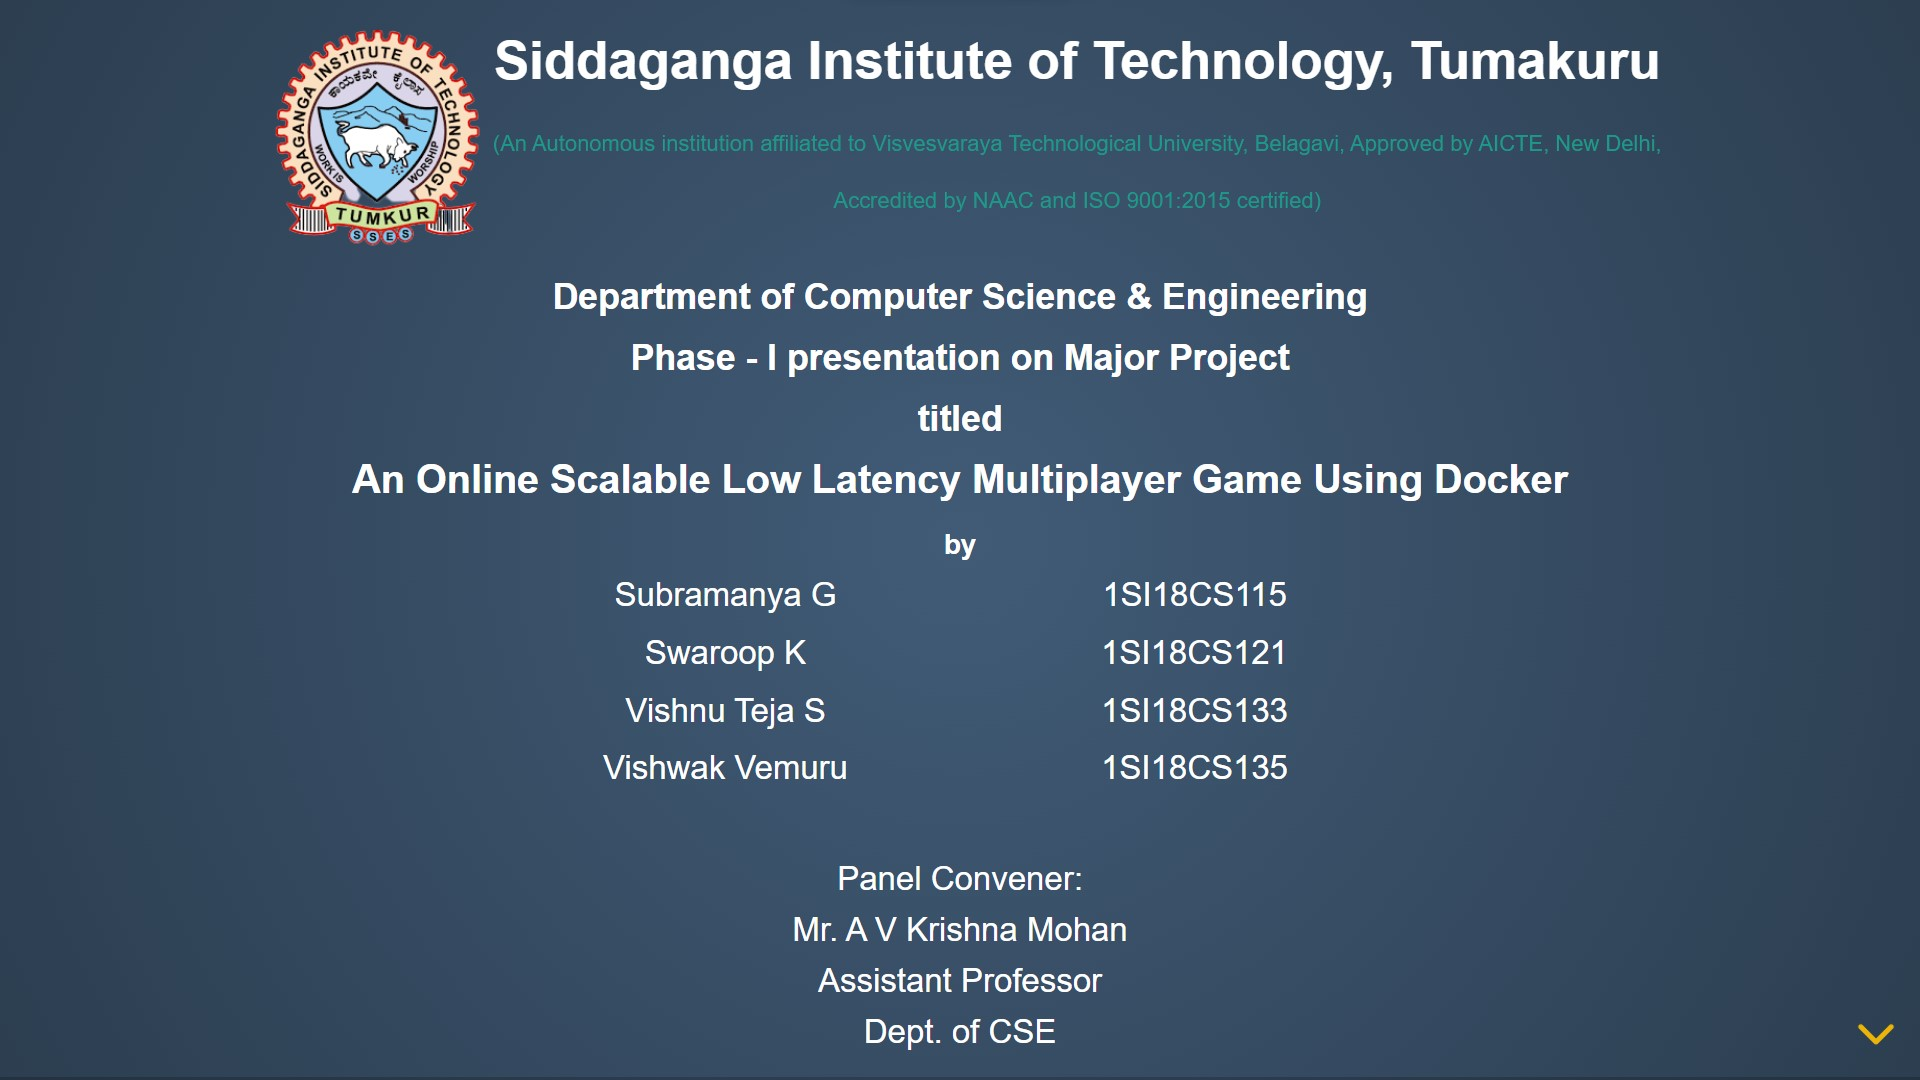
\includegraphics[scale=0.22]{s1.jpg}\vfill
		%\newline
		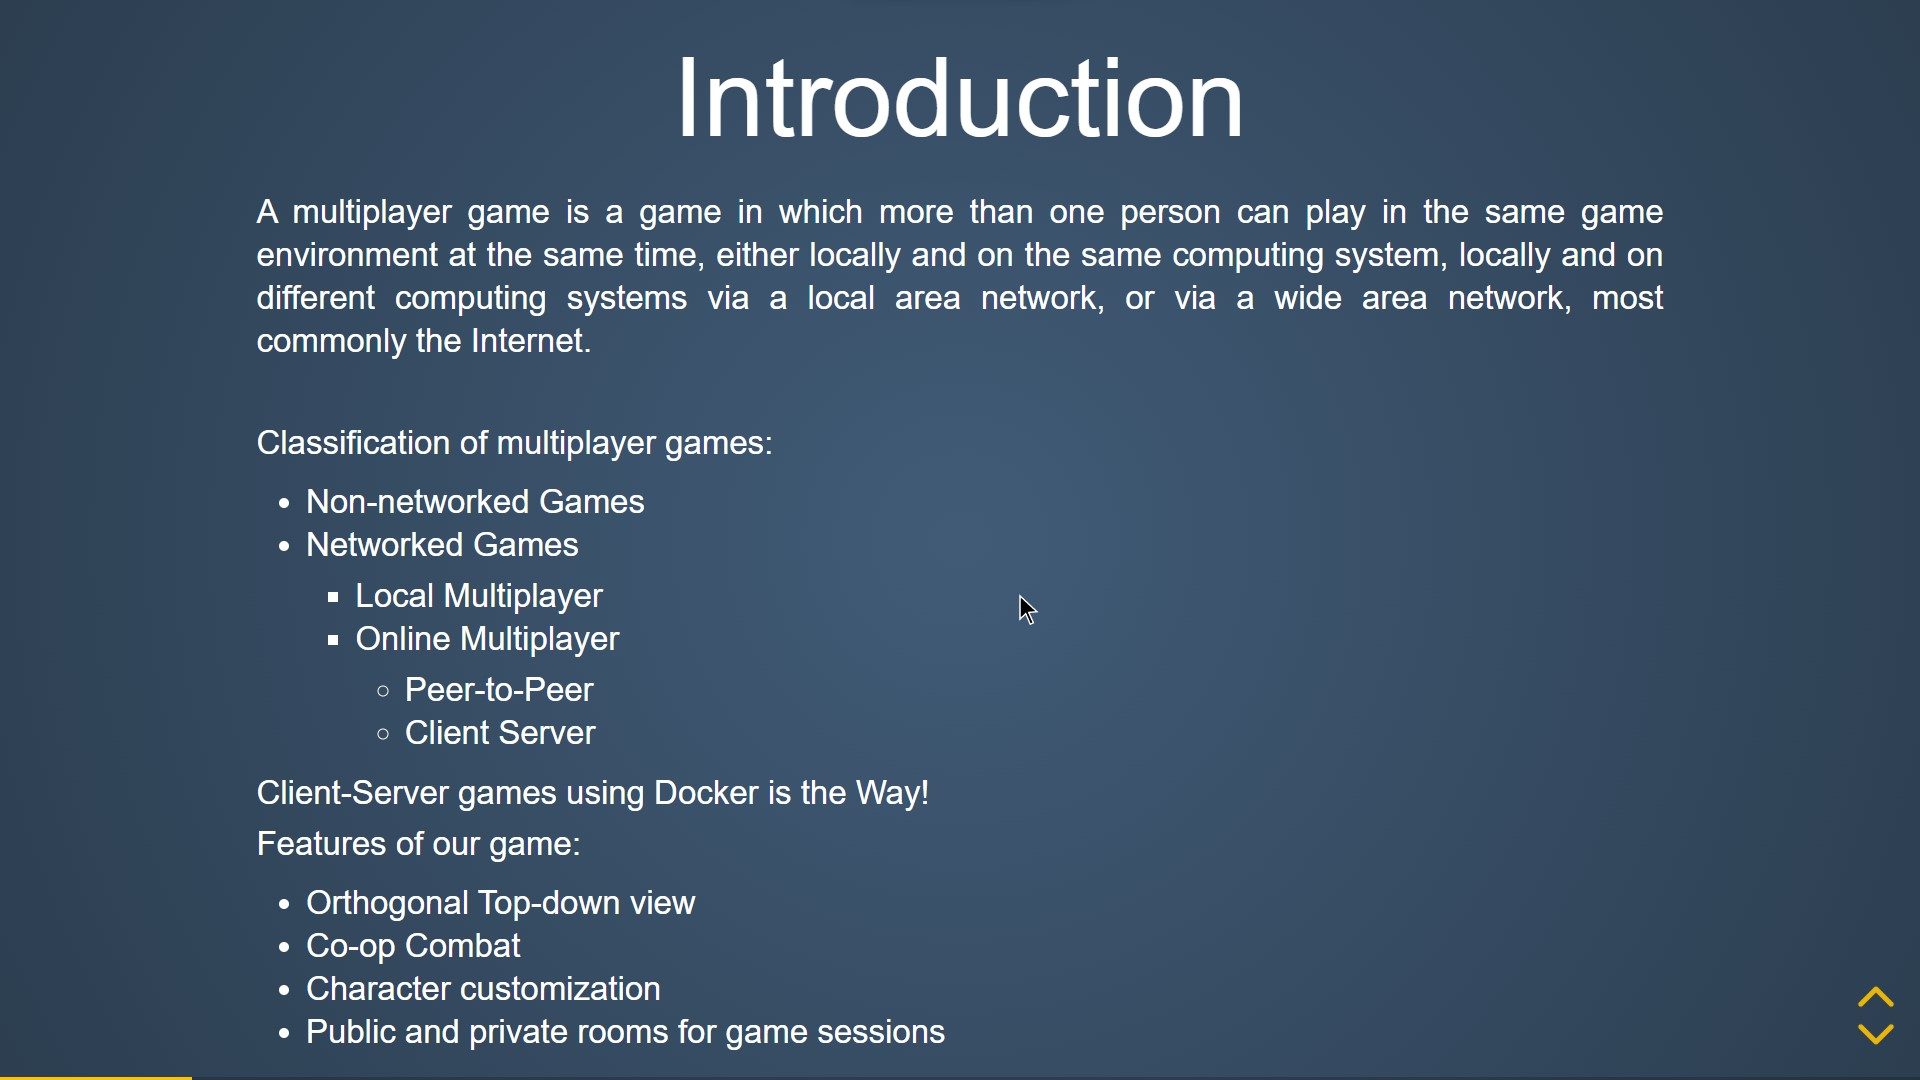
\includegraphics[scale=0.22]{s2.jpg}\vfill
		%\newline
		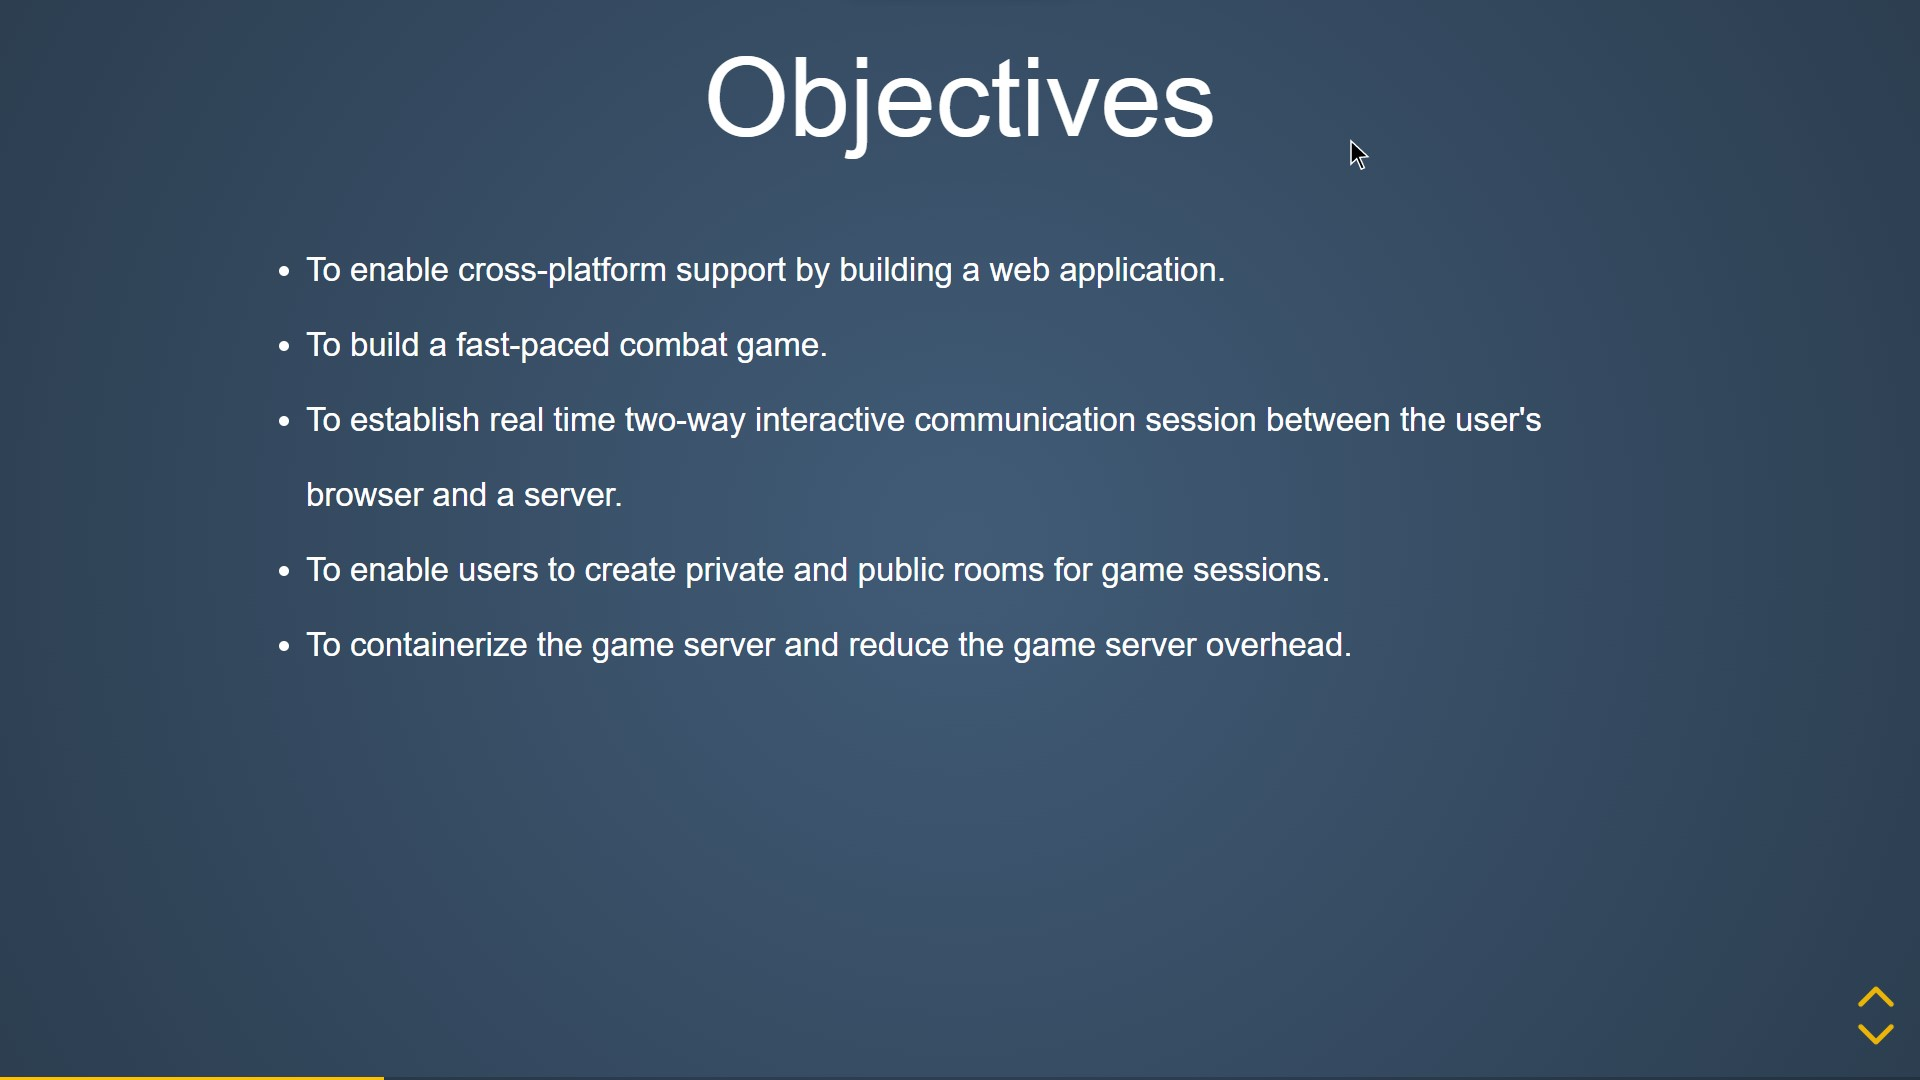
\includegraphics[scale=0.22]{s3.jpg}\vfill
		%\newline
		%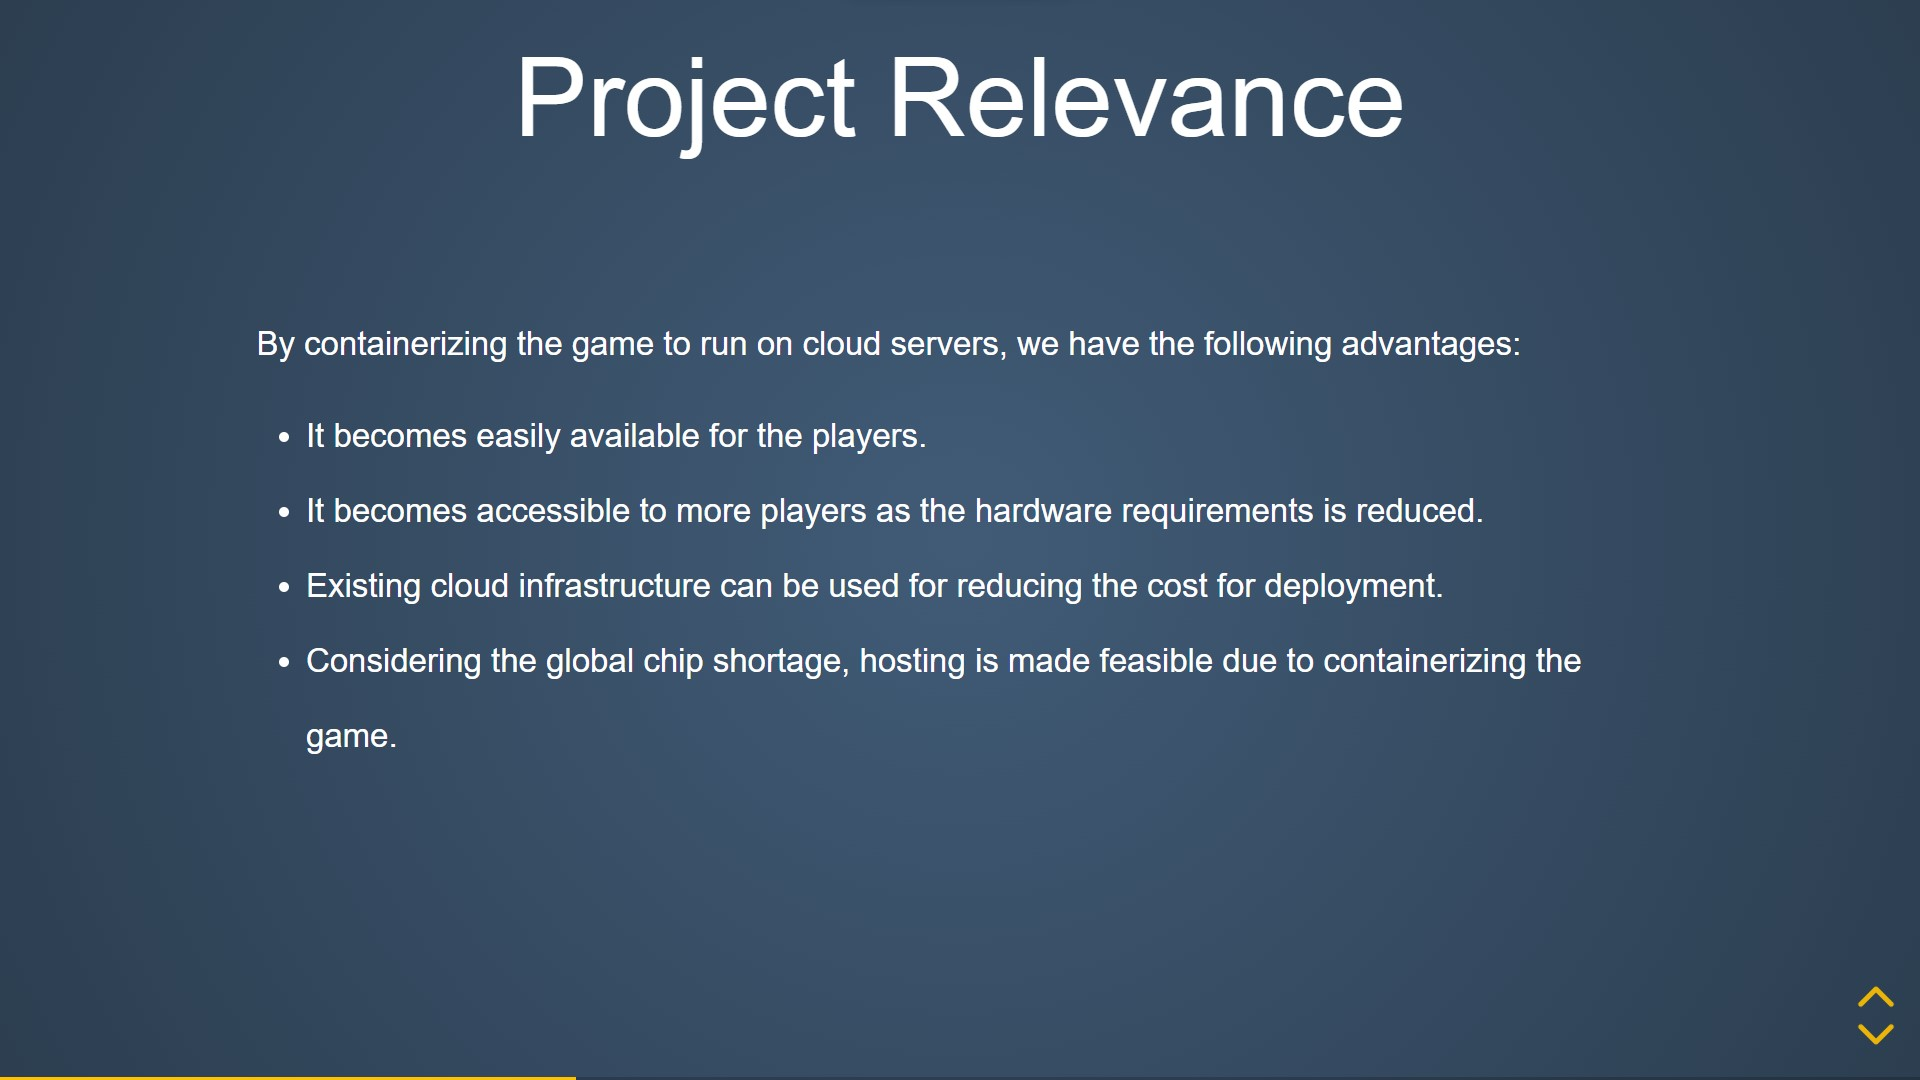
\includegraphics[scale=0.16]{s4.jpg}
	\end{figure}
	\pagebreak
	\begin{figure}[ht!]
		\centering
		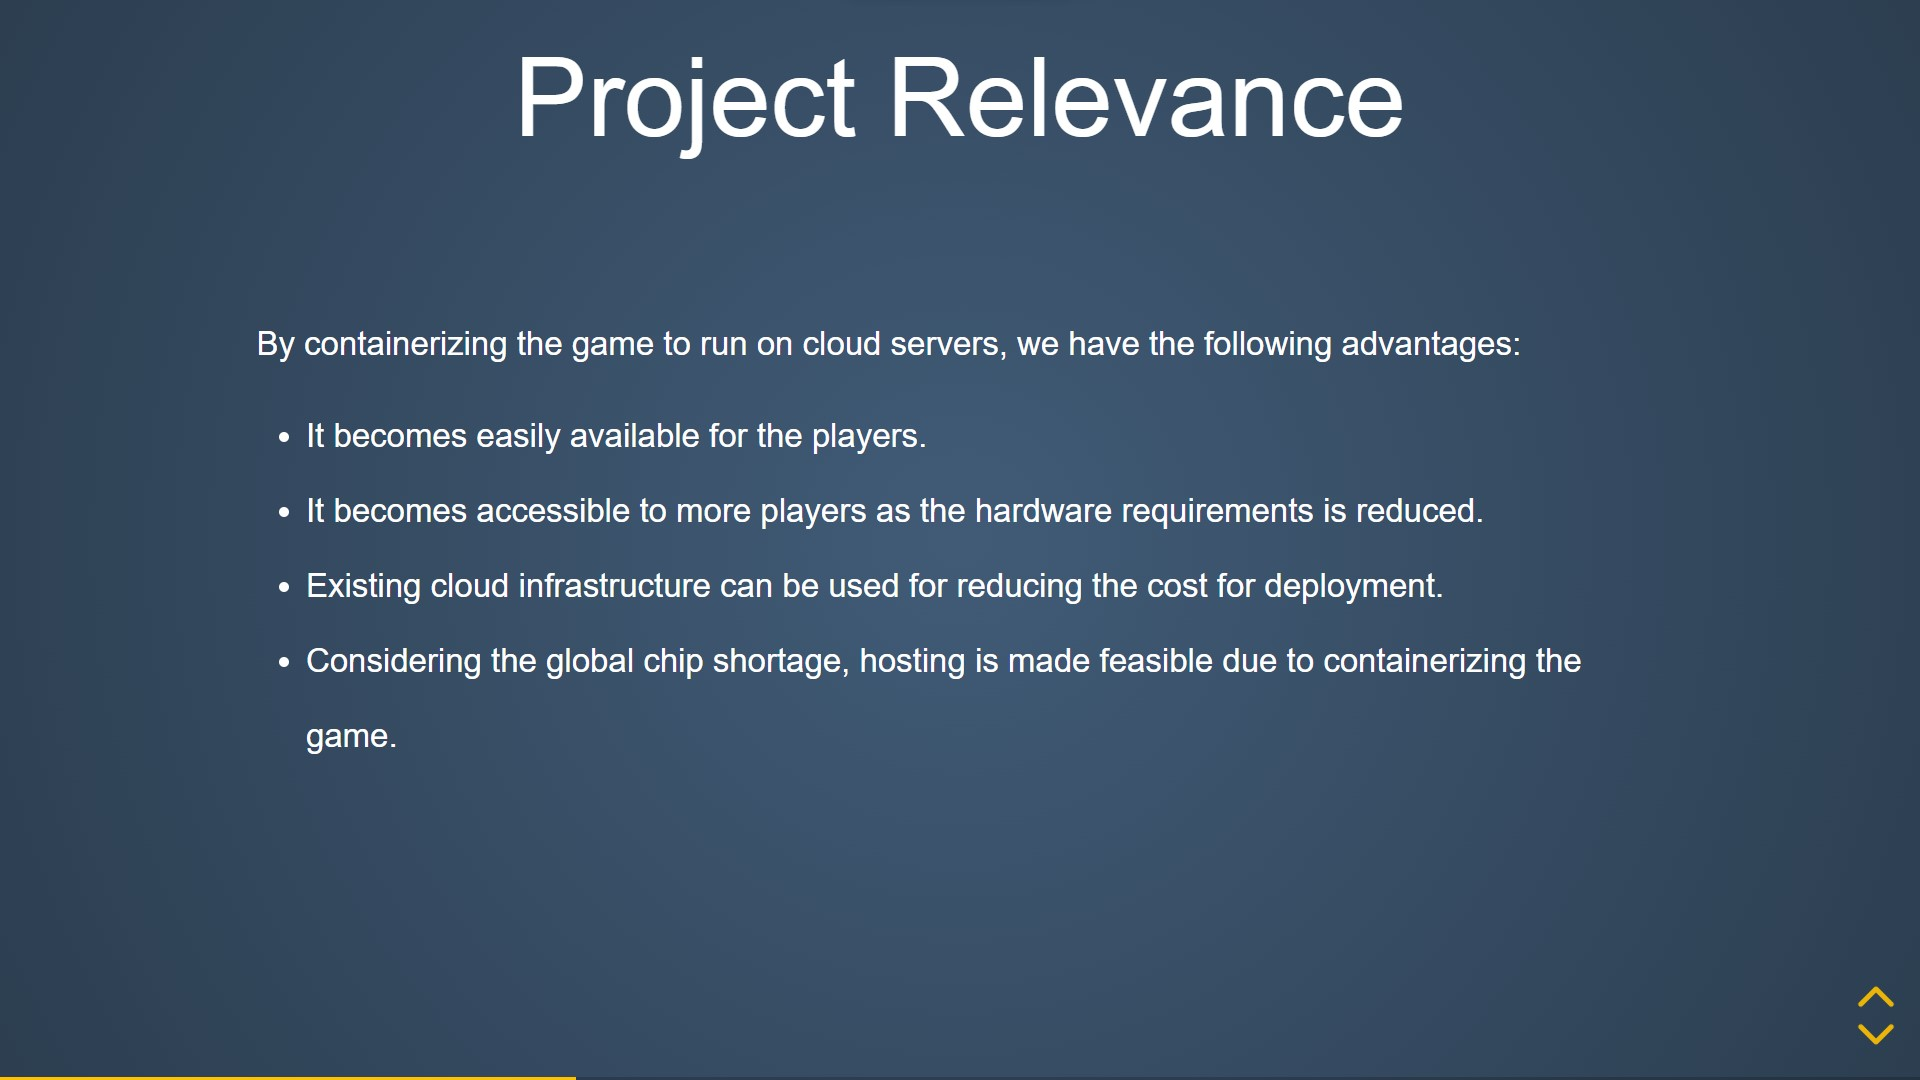
\includegraphics[scale=0.22]{s4.jpg}\vfill
		%\newline
		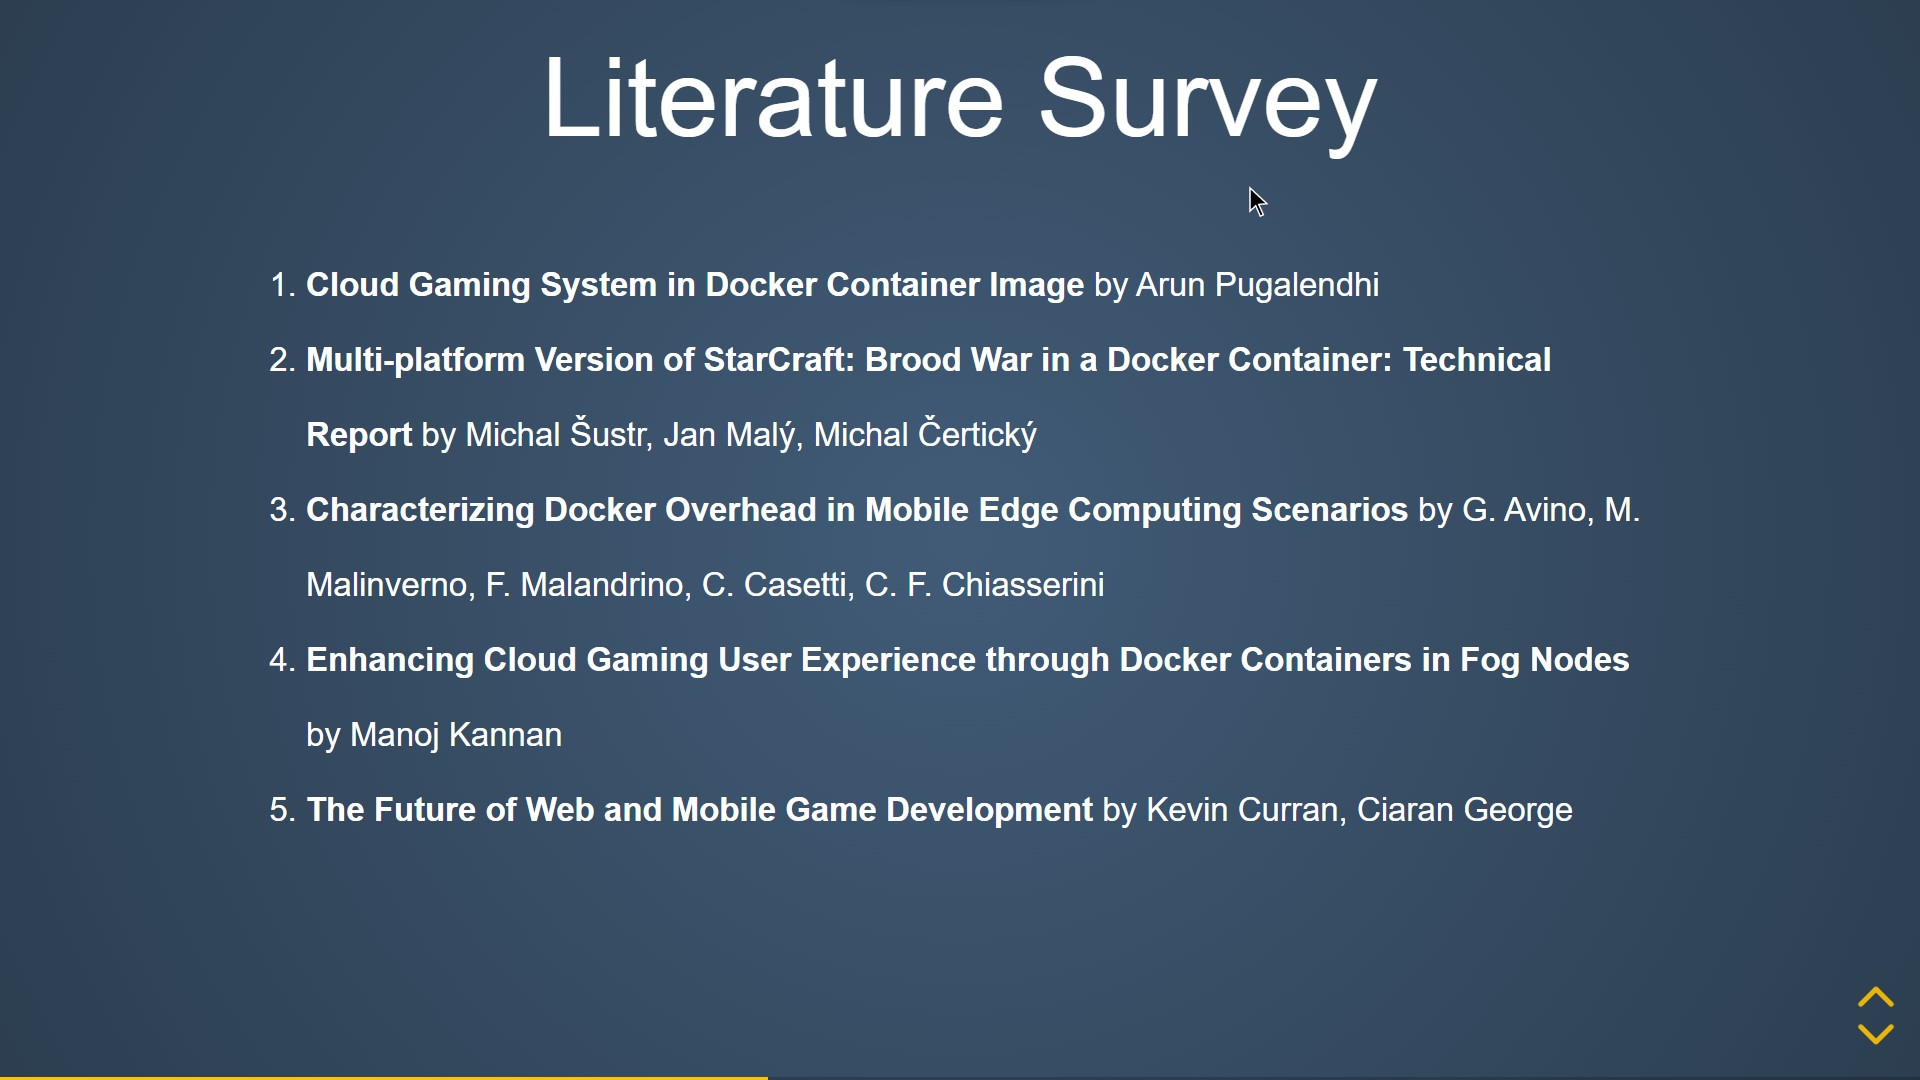
\includegraphics[scale=0.22]{s5.jpg}\vfill
		%\newline
		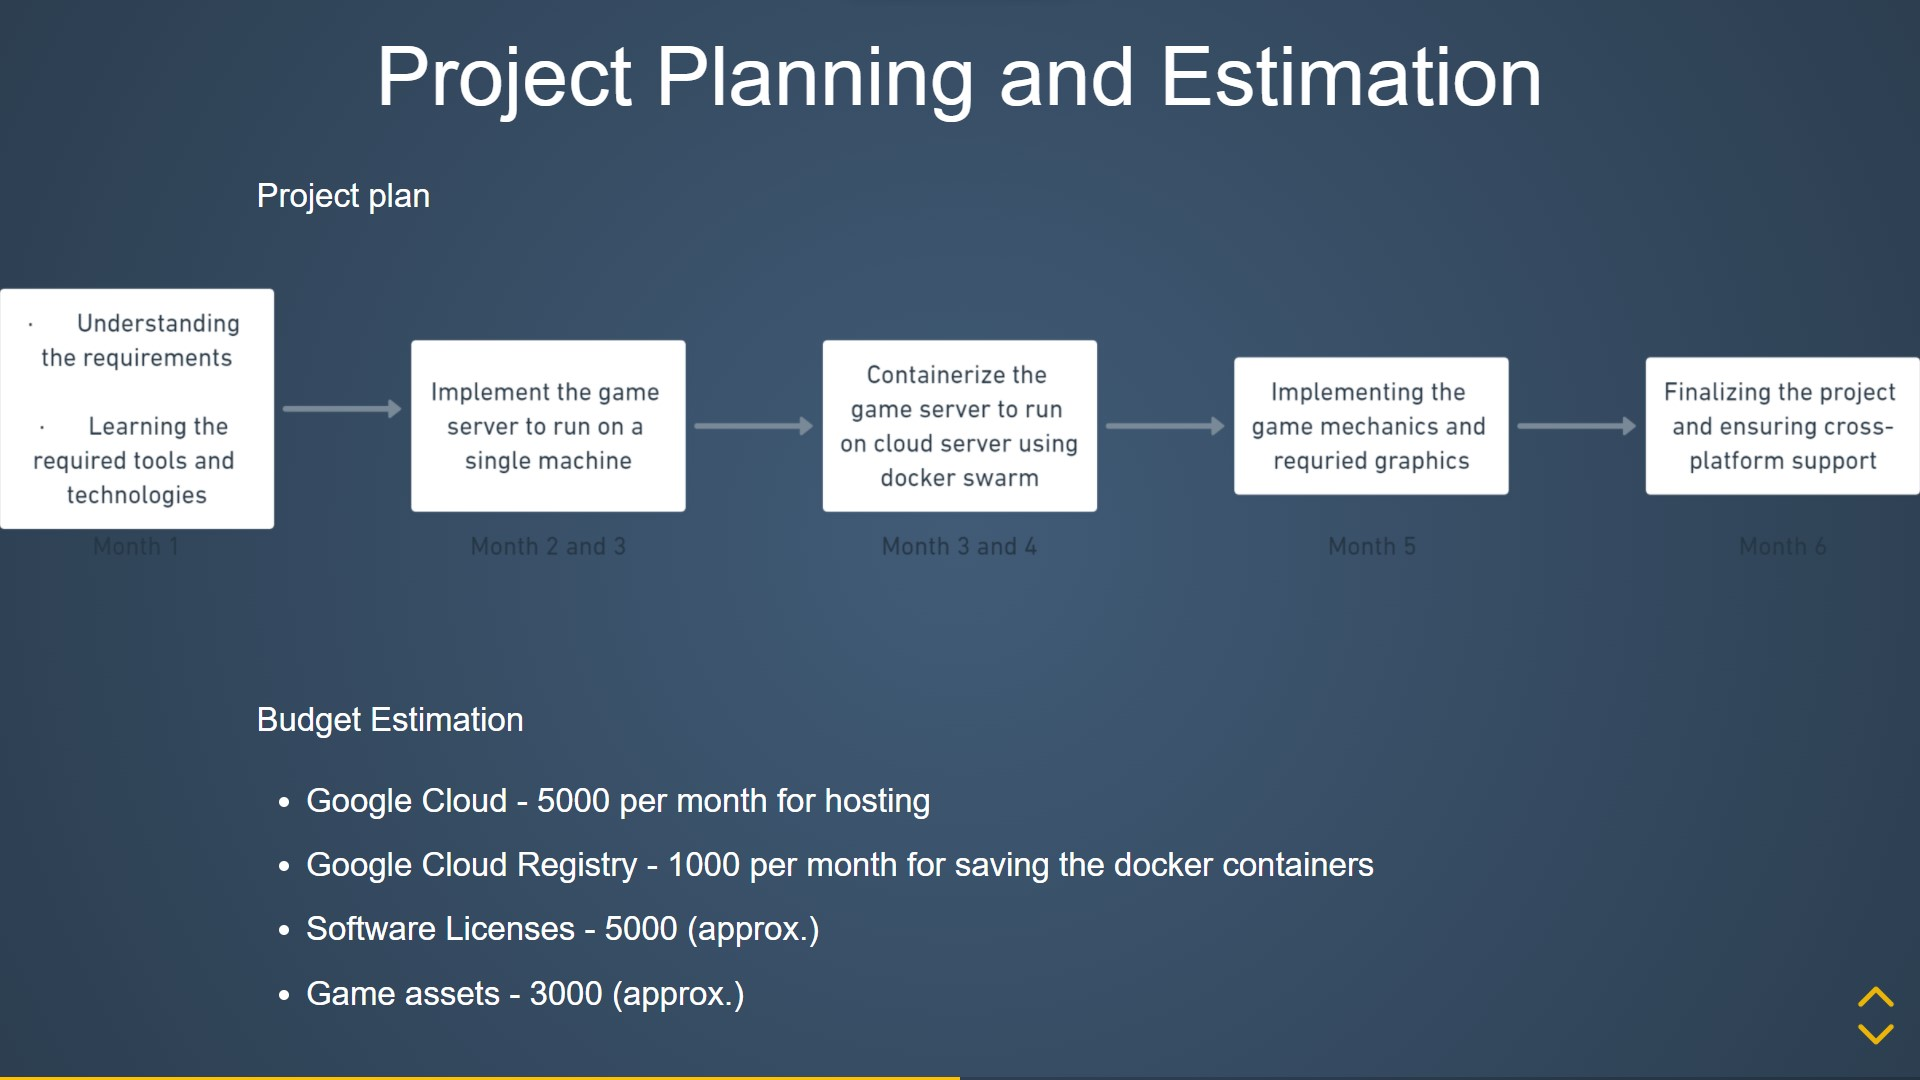
\includegraphics[scale=0.22]{s6.jpg}\vfill
		%\newline
		%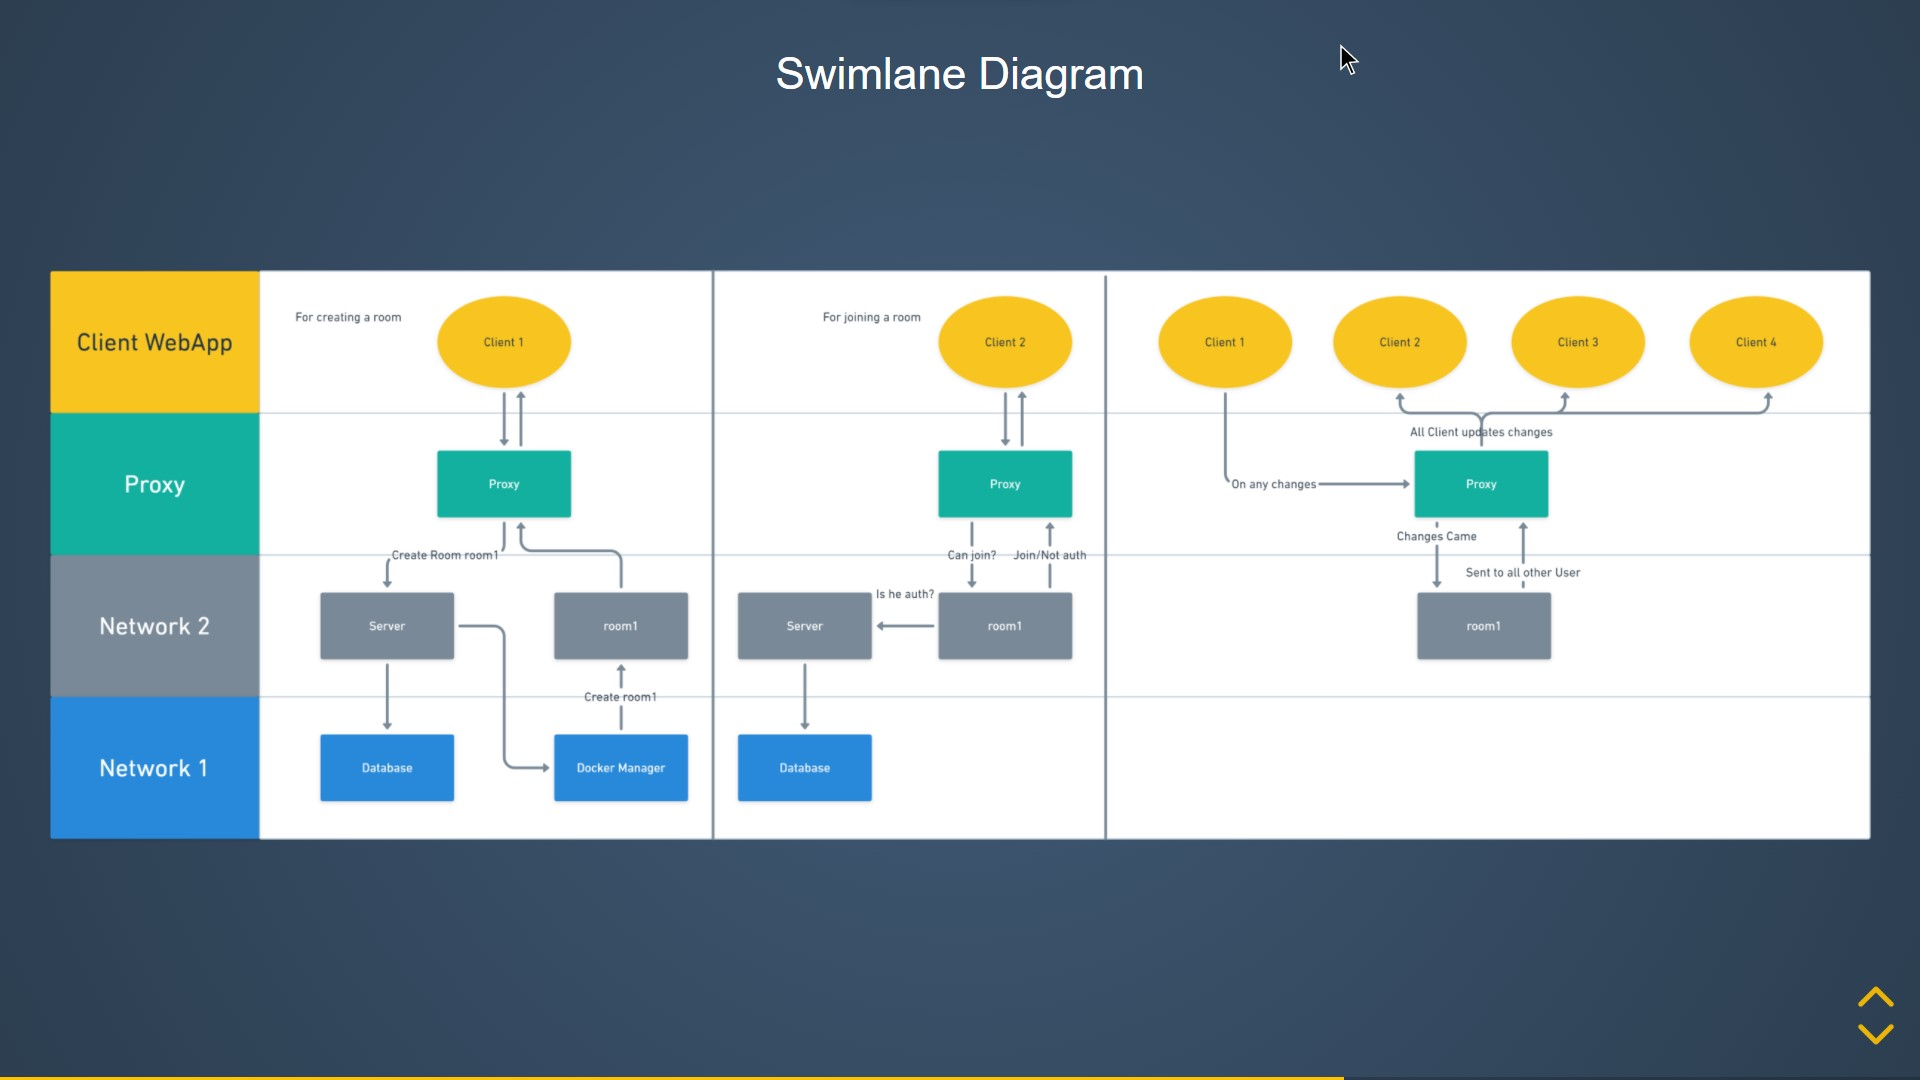
\includegraphics[scale=0.16]{s8.jpg}
	\end{figure}
	\pagebreak
	\begin{figure}[ht!]
		\centering
		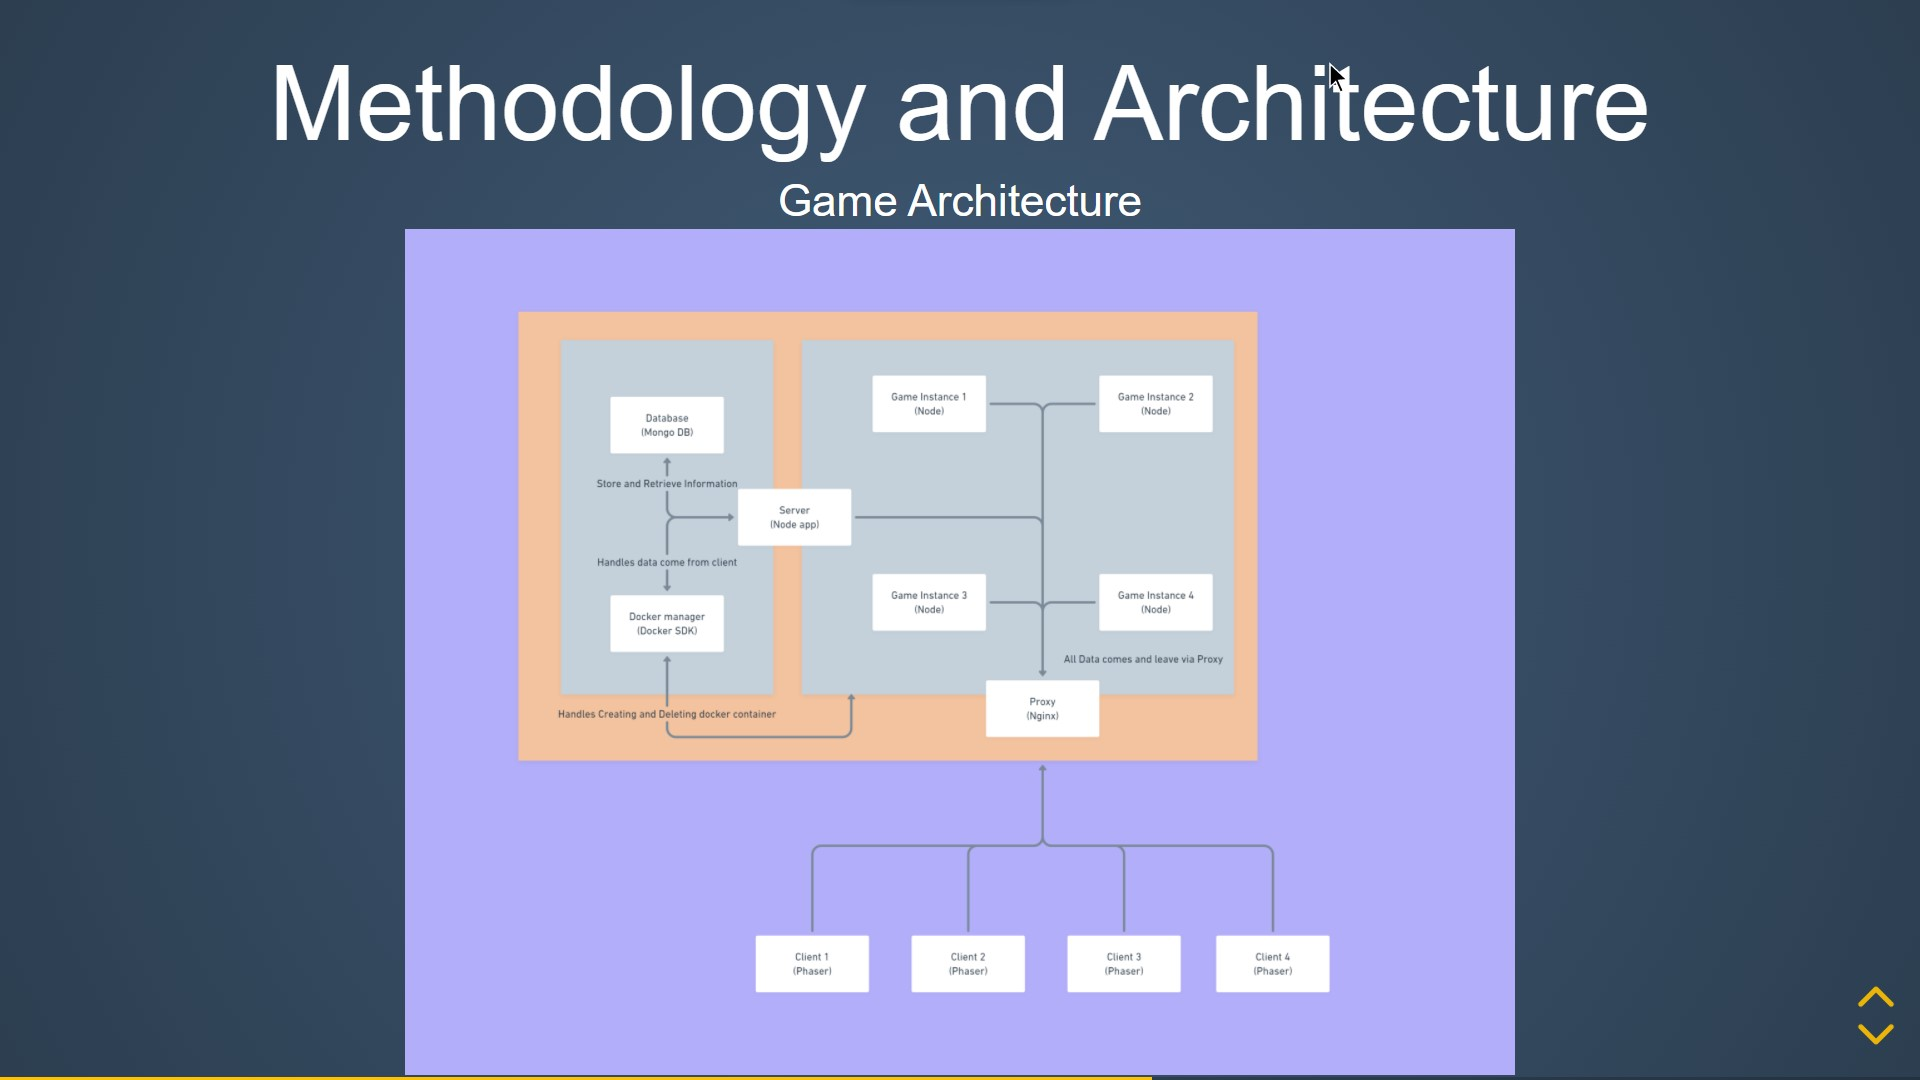
\includegraphics[scale=0.22]{s7.jpg}
		%\newline
		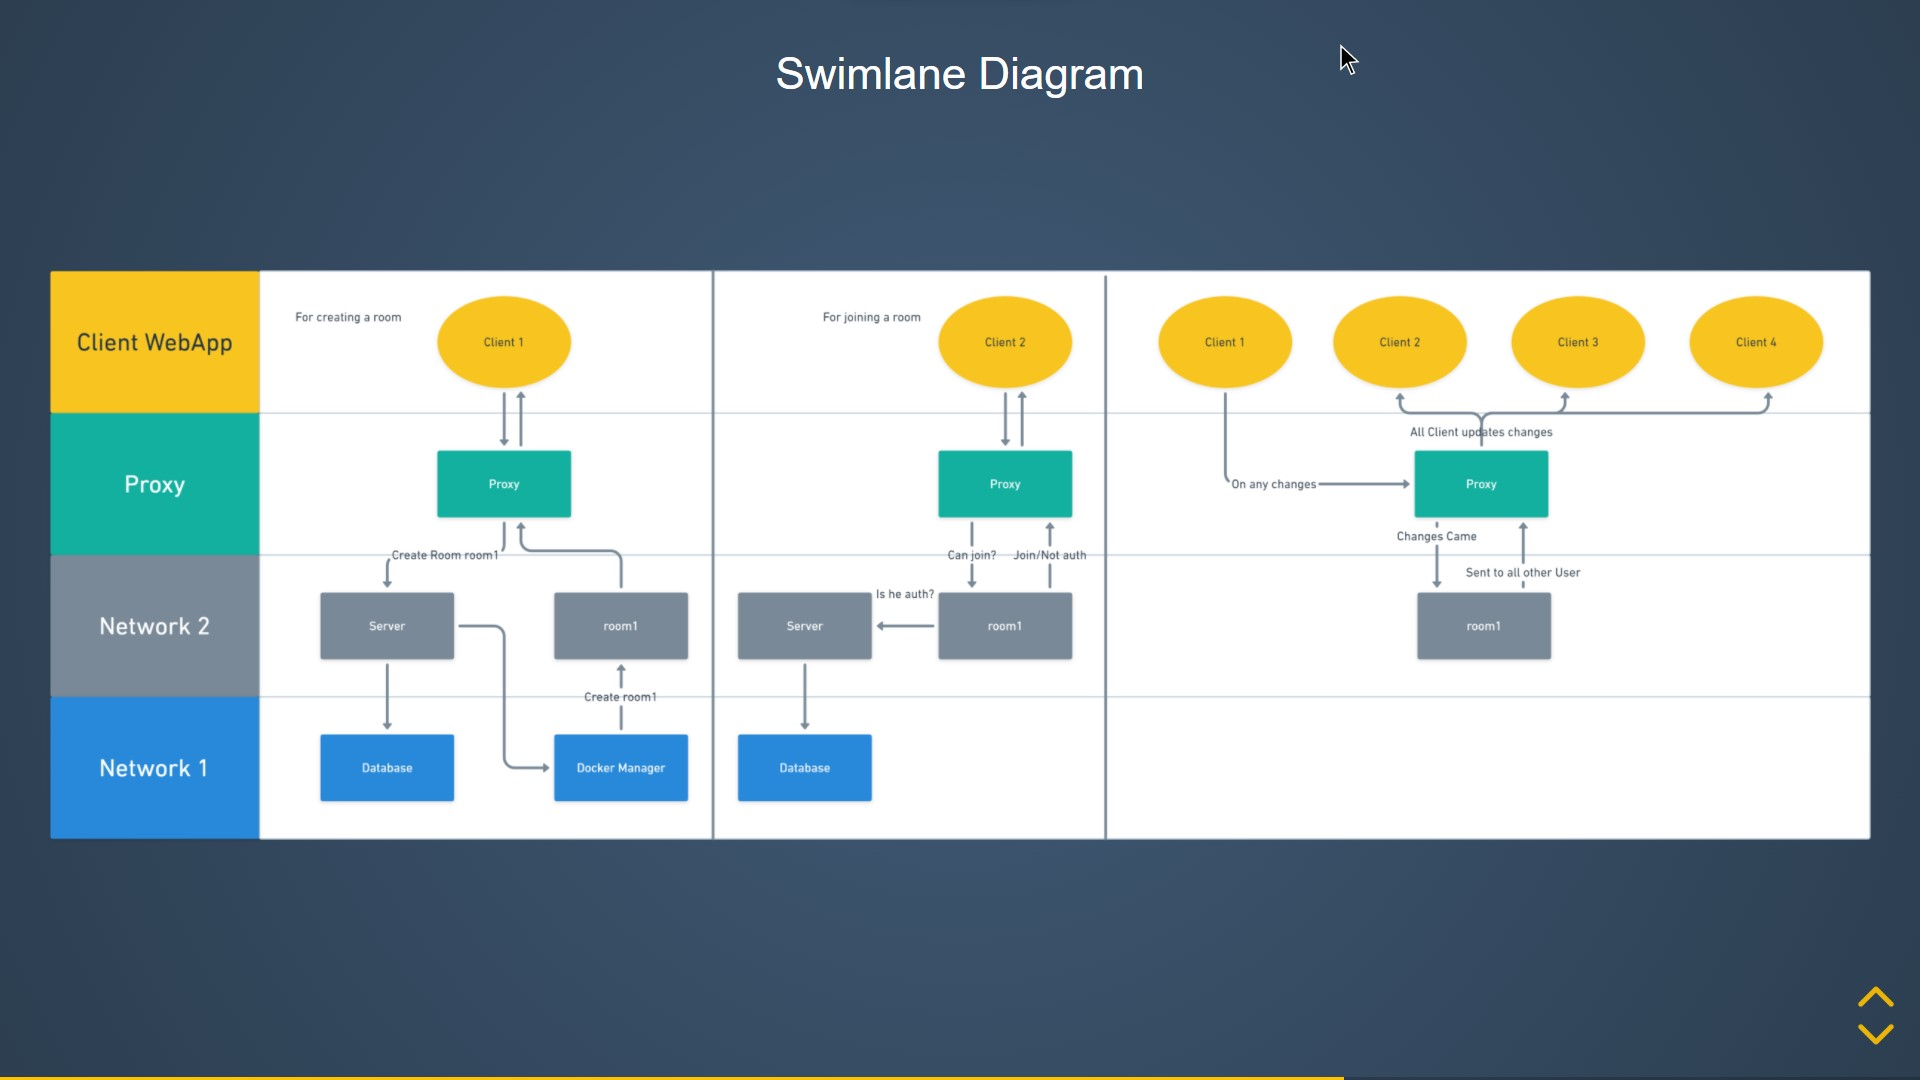
\includegraphics[scale=0.22]{s8.jpg}
		%\newline
		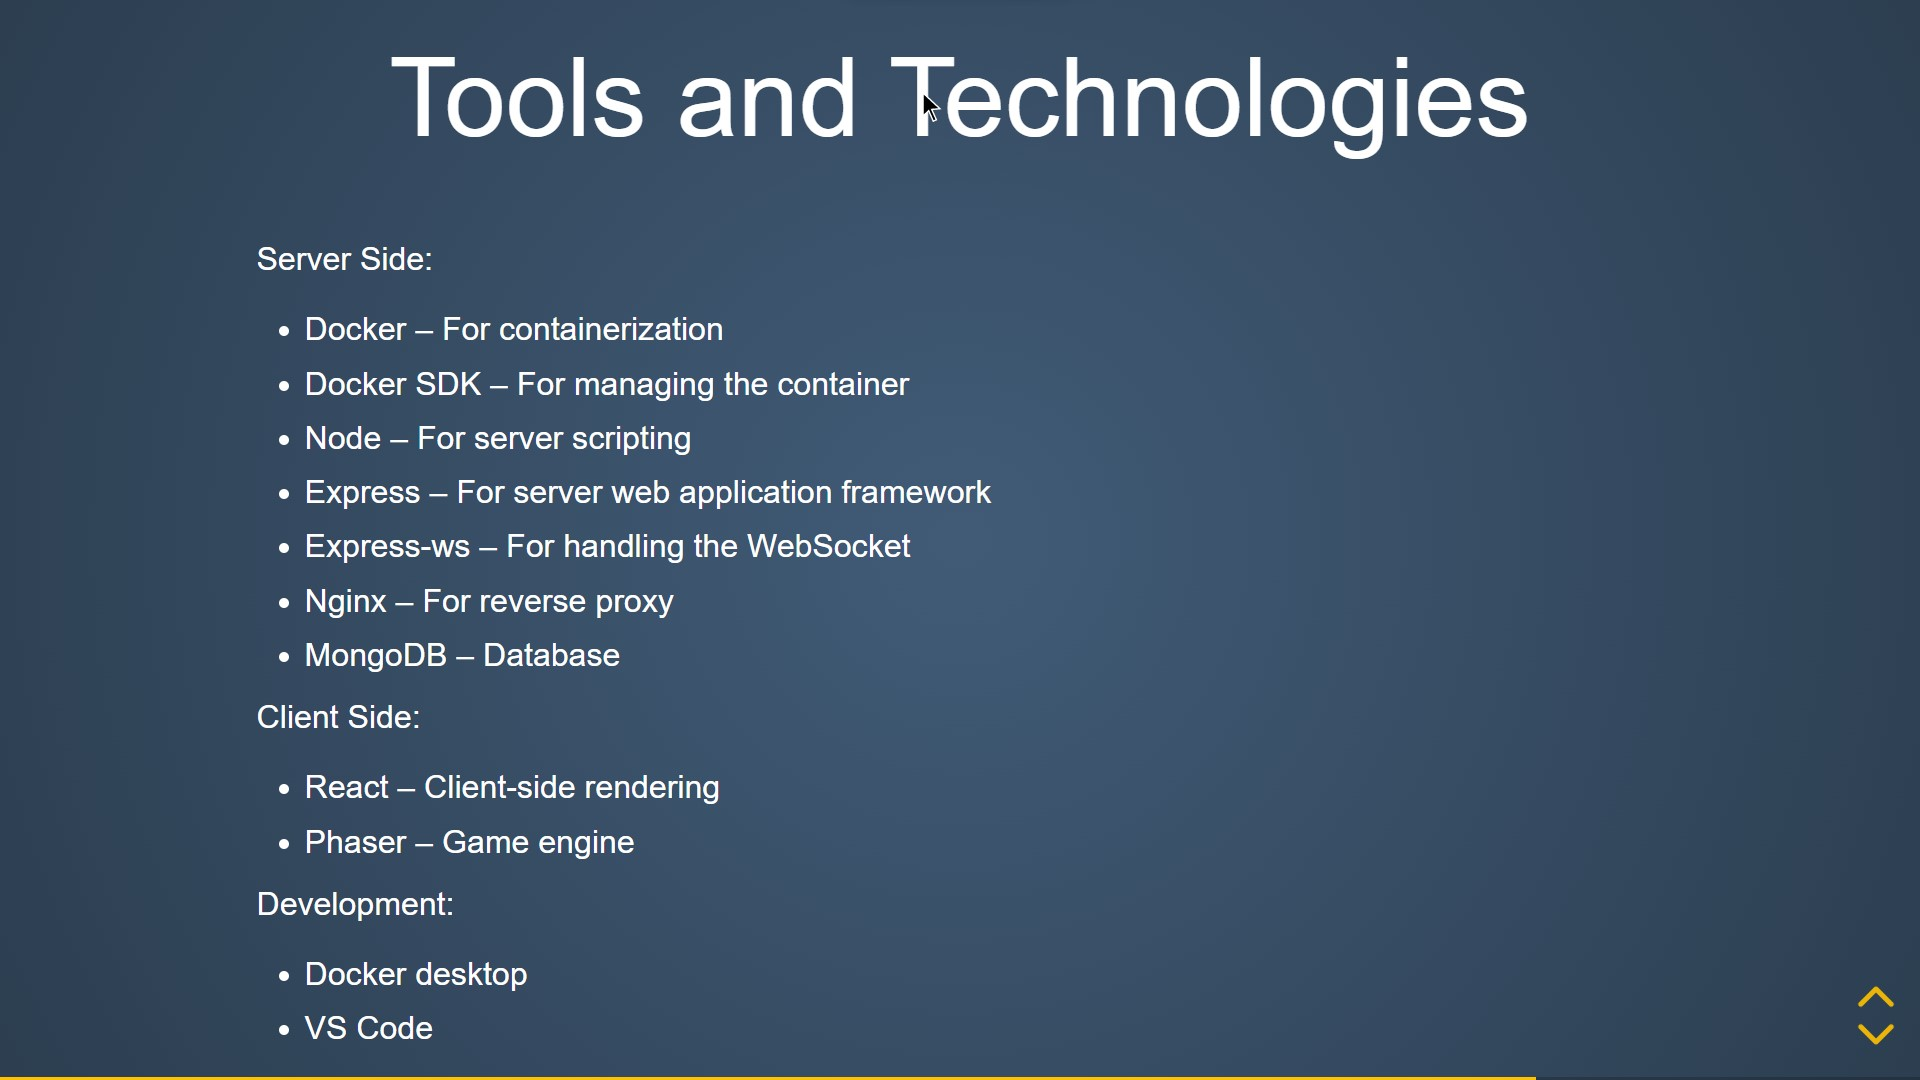
\includegraphics[scale=0.22]{s9.jpg}
		%\newline
	\end{figure}
	\pagebreak
	\begin{figure}[ht!]
		\centering
		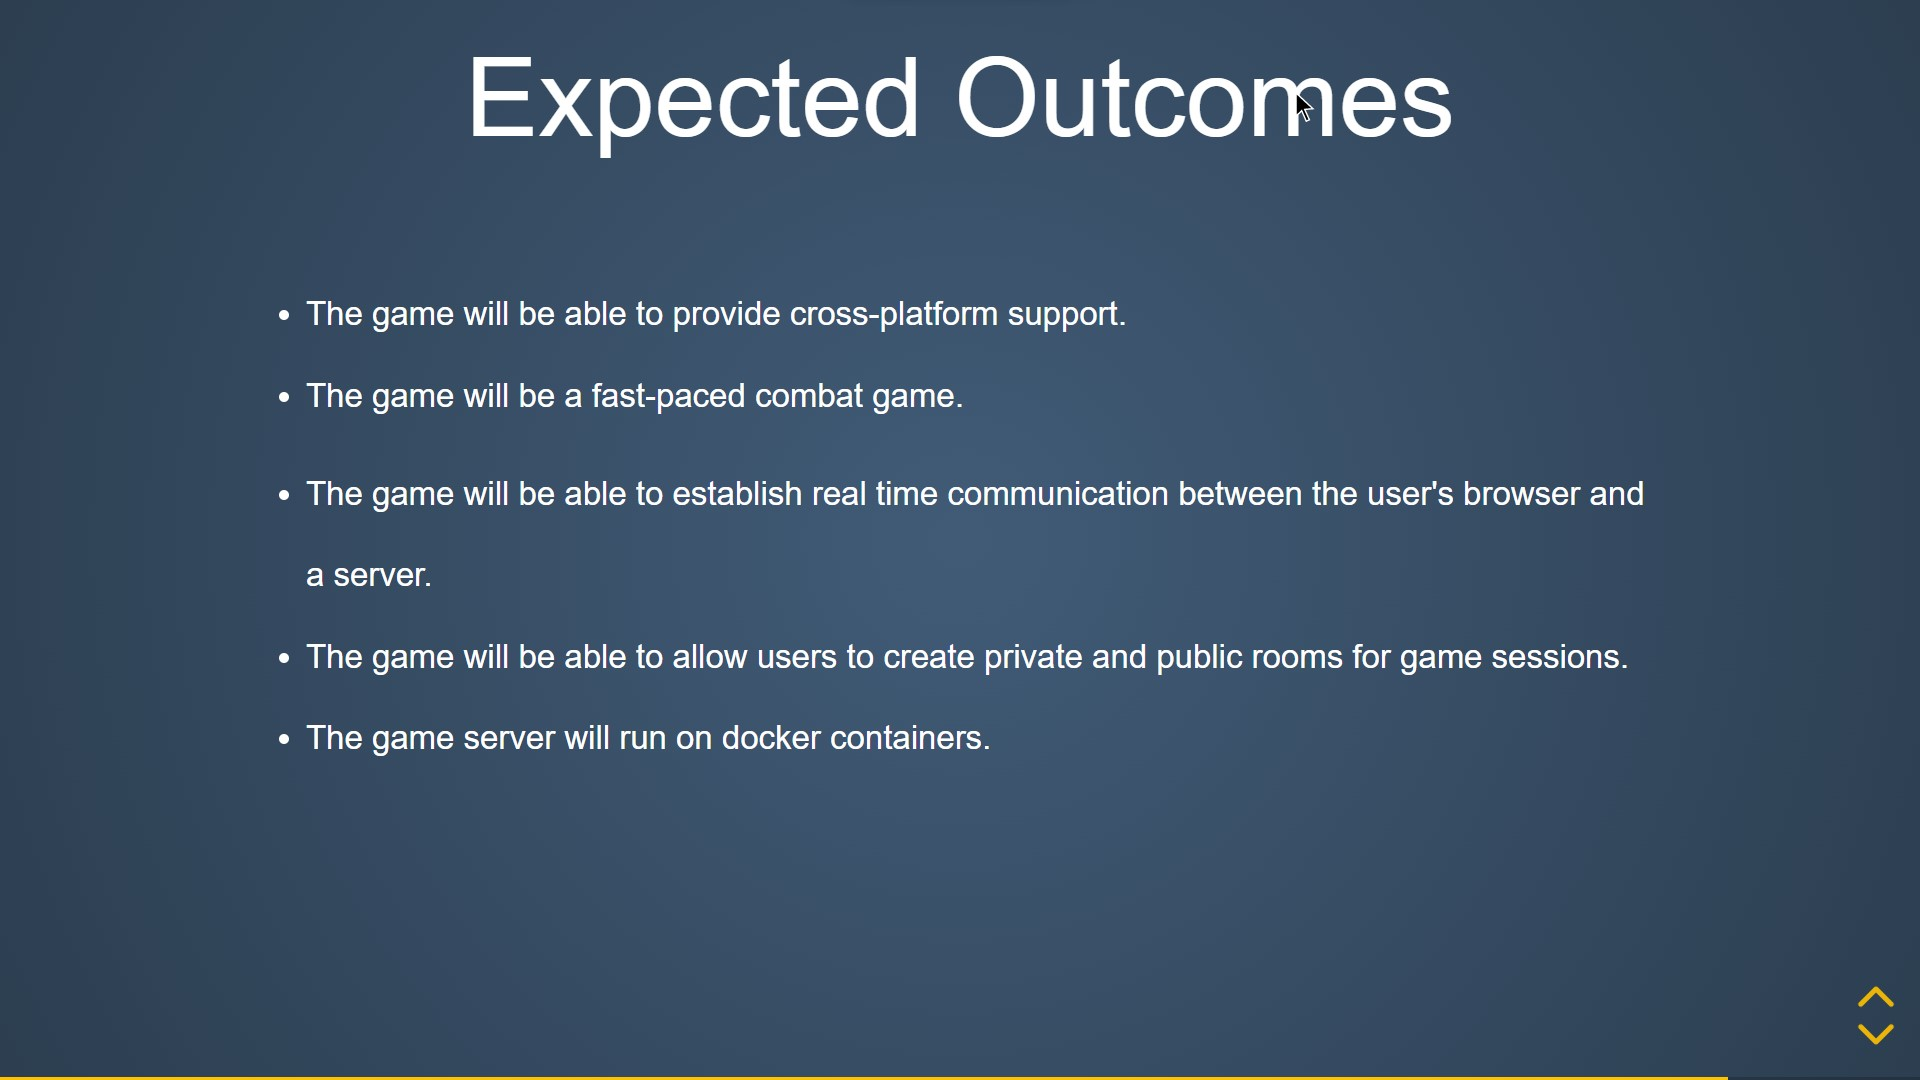
\includegraphics[scale=0.25]{s10.jpg}
		%\newline
		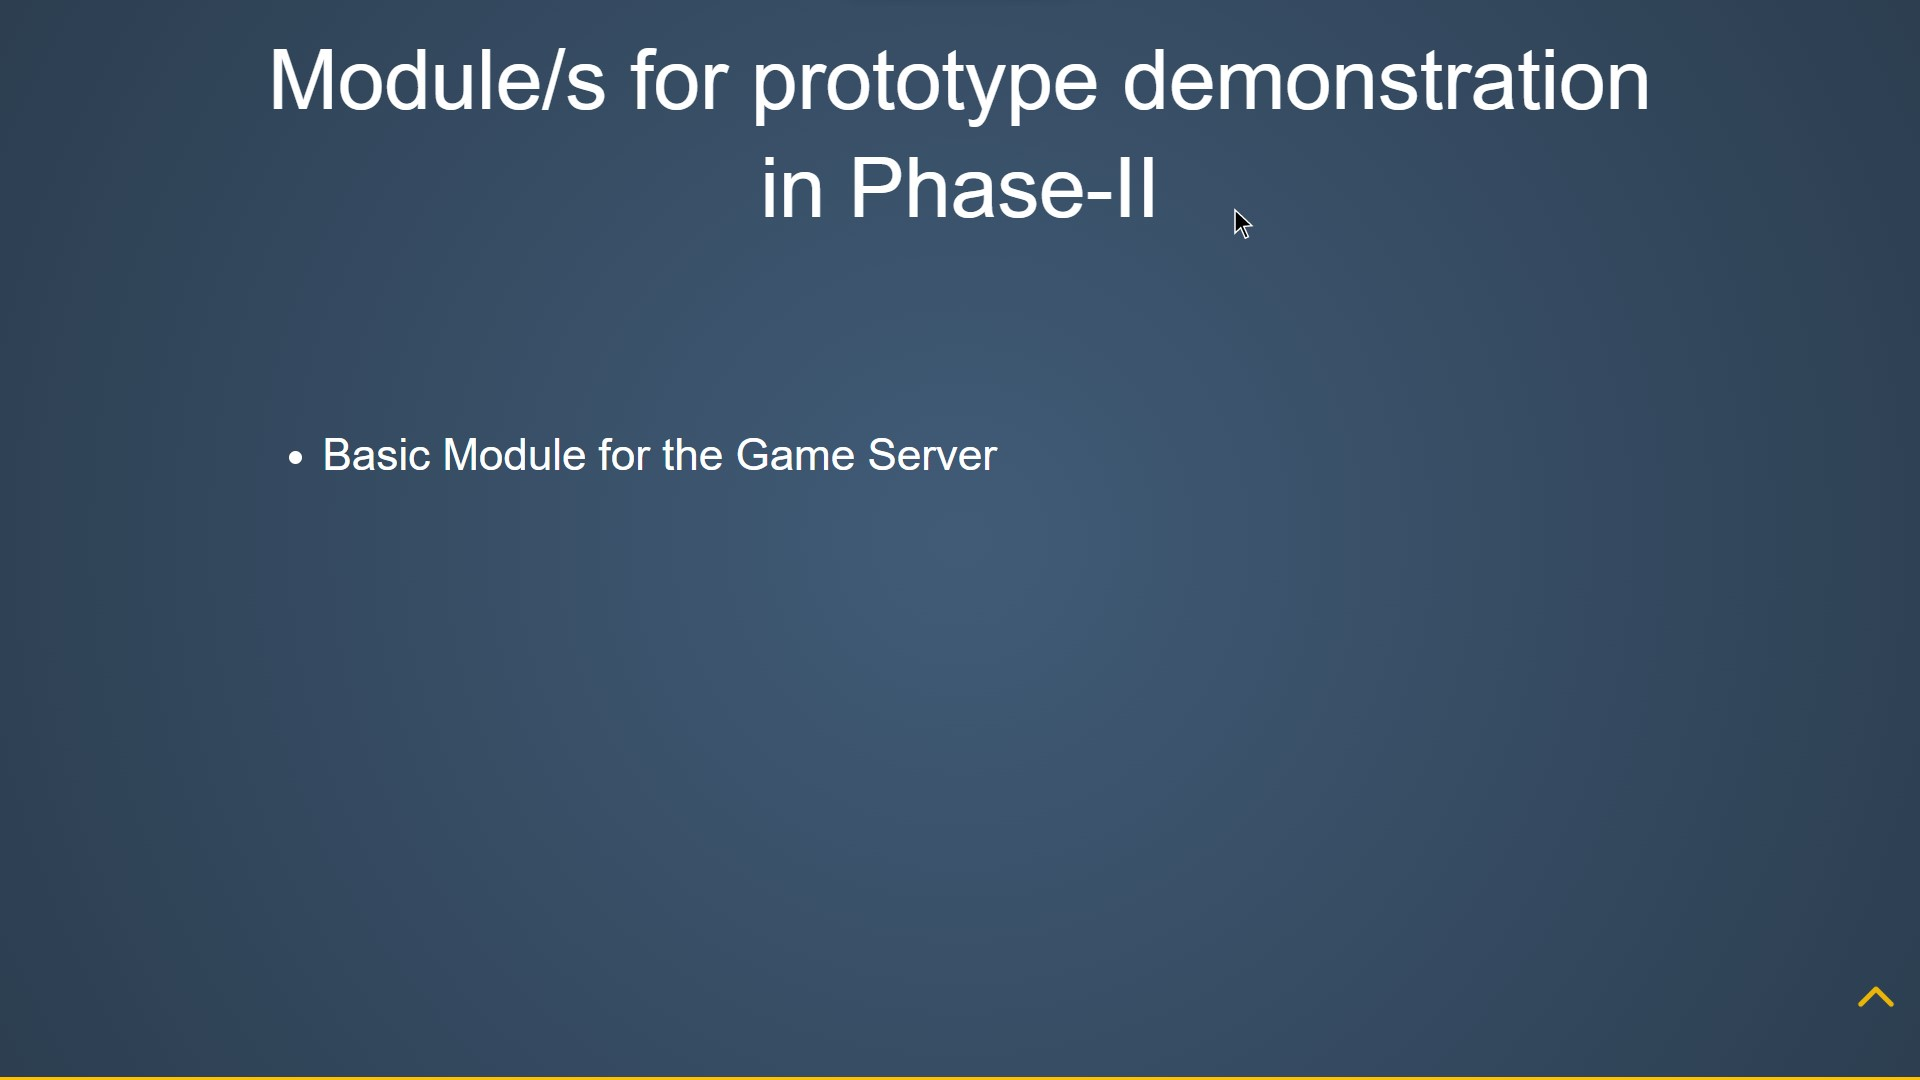
\includegraphics[scale=0.25]{s11.jpg}
	\end{figure}

\pagebreak

\addcontentsline{toc}{chapter}{Phase II Presentation Slides}
\section*{Phase II Presentation Slides}
	\begin{figure}[ht!]
		\centering
		
\includegraphics[scale=0.3]{0001.jpg}\vfill
		%\newline
		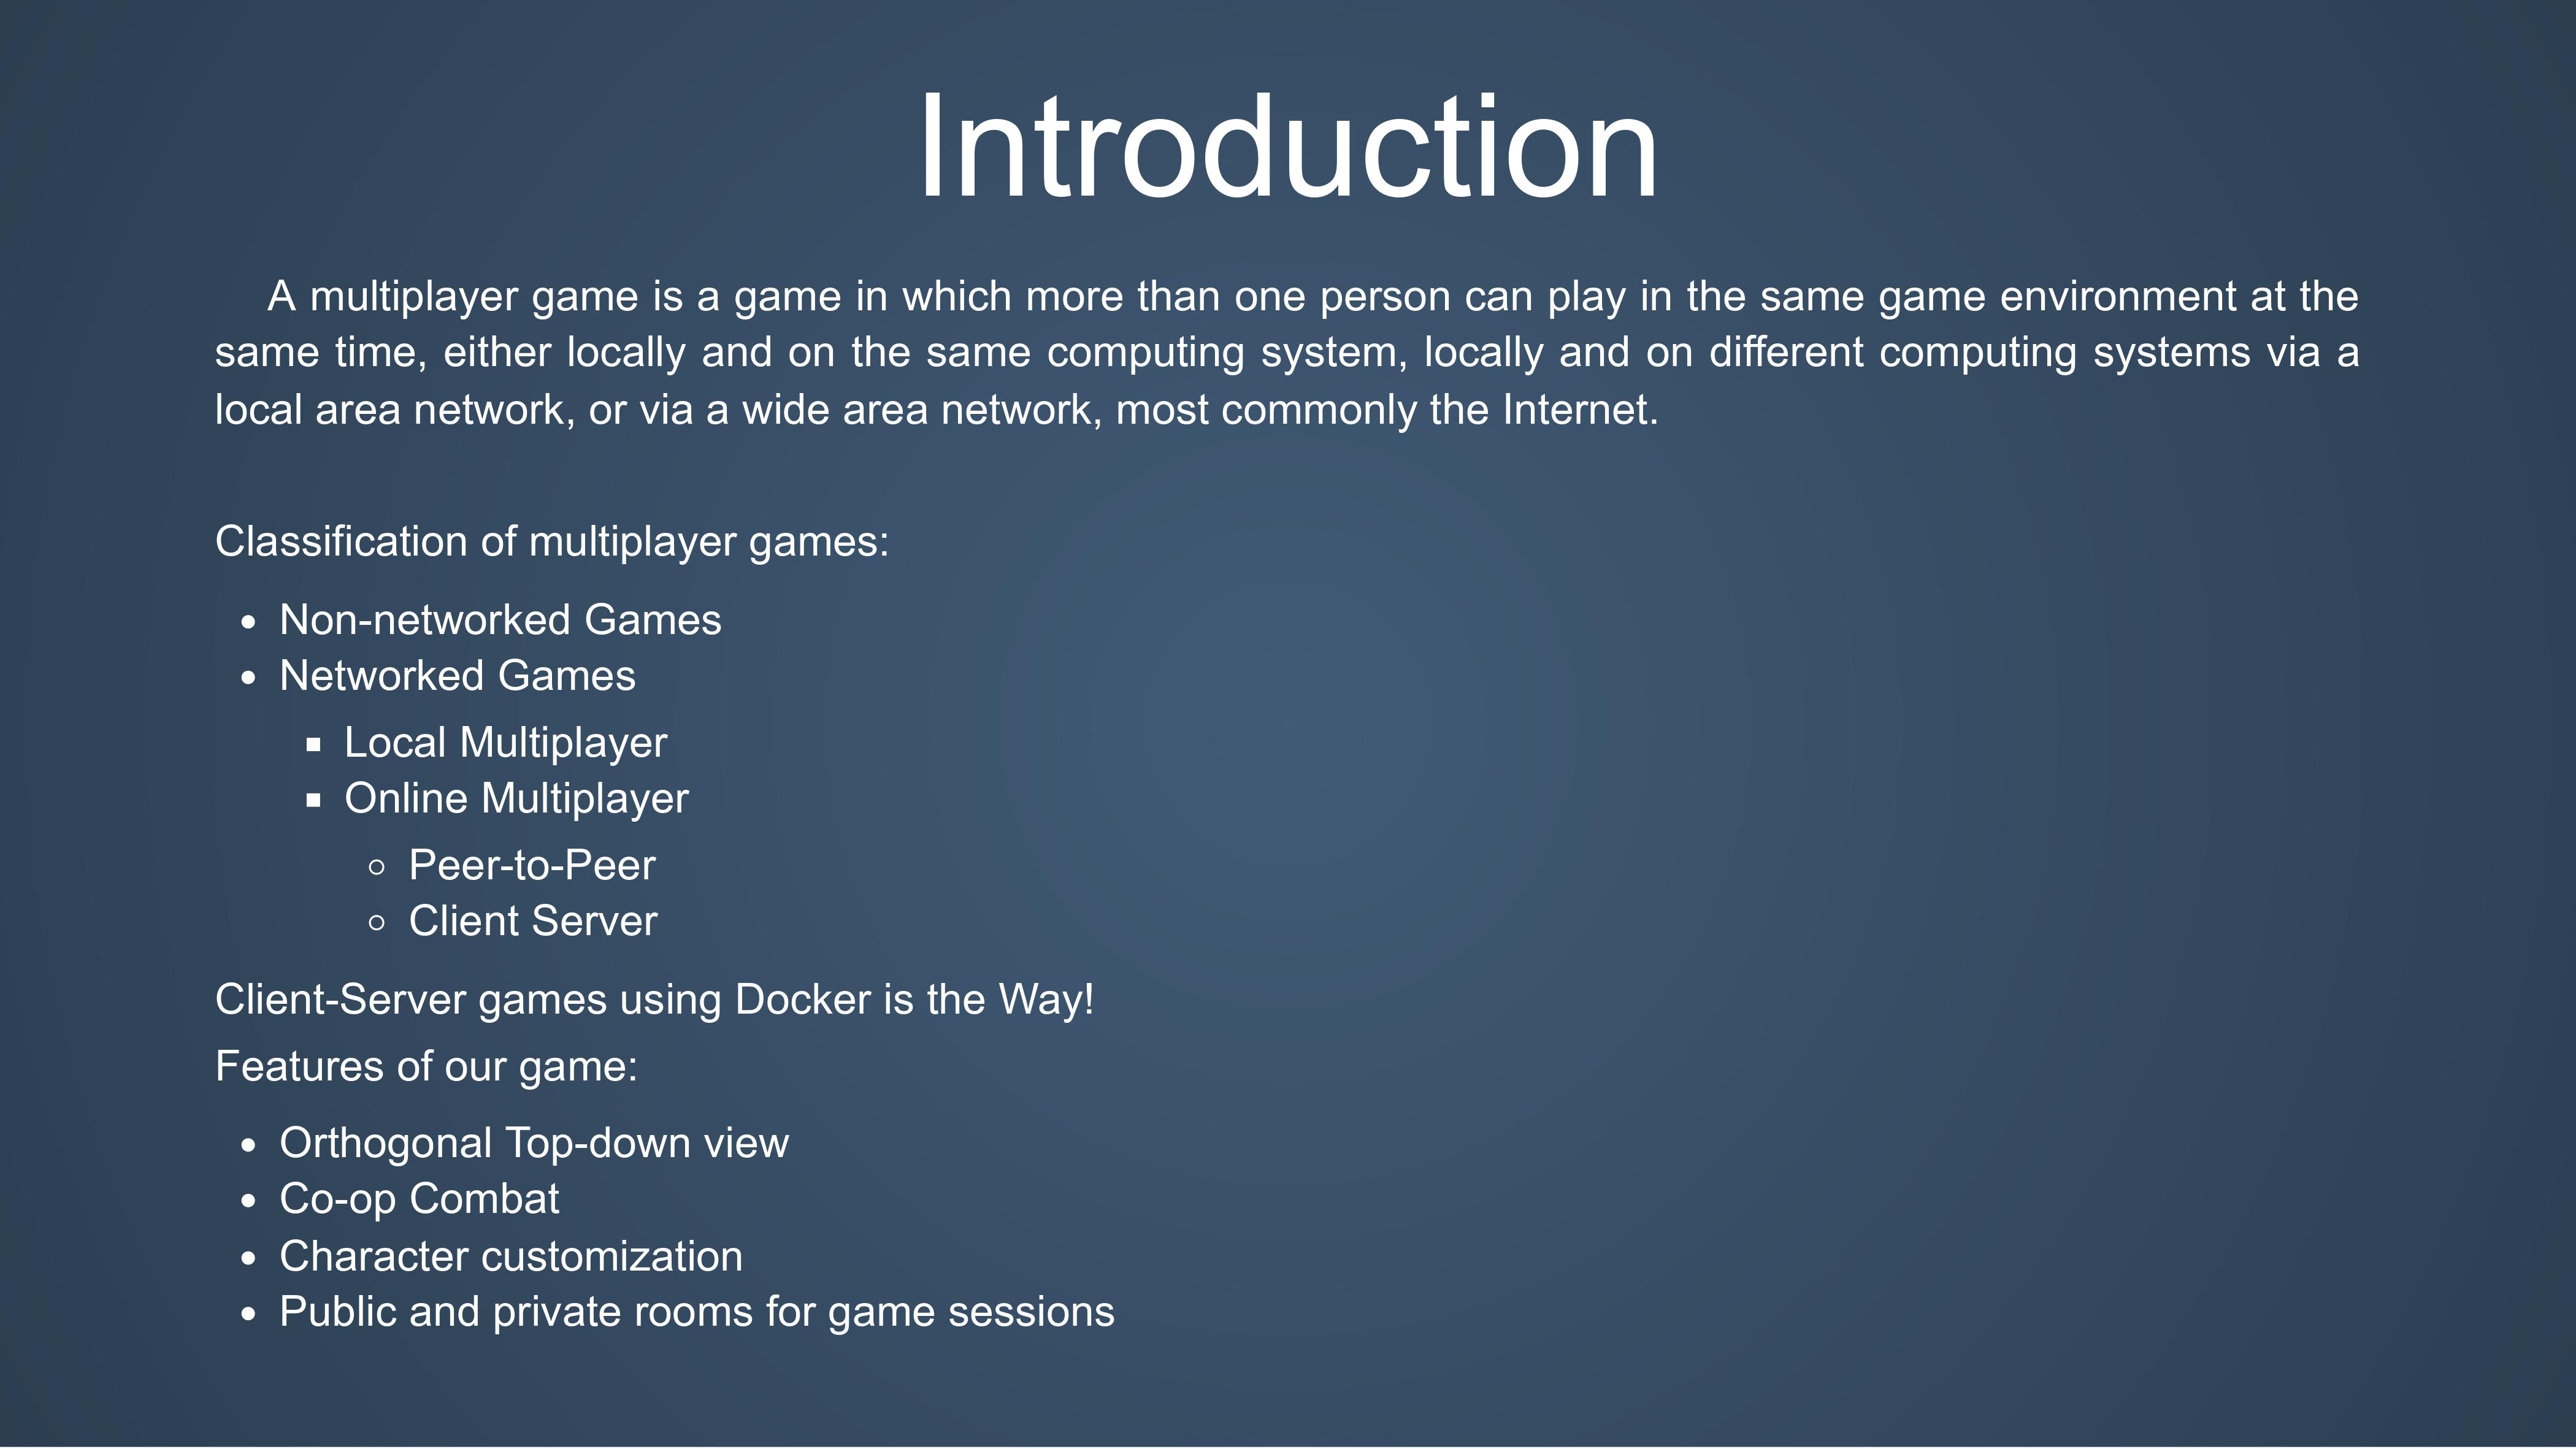
\includegraphics[scale=0.3]{0002.jpg}\vfill
		%\newline
		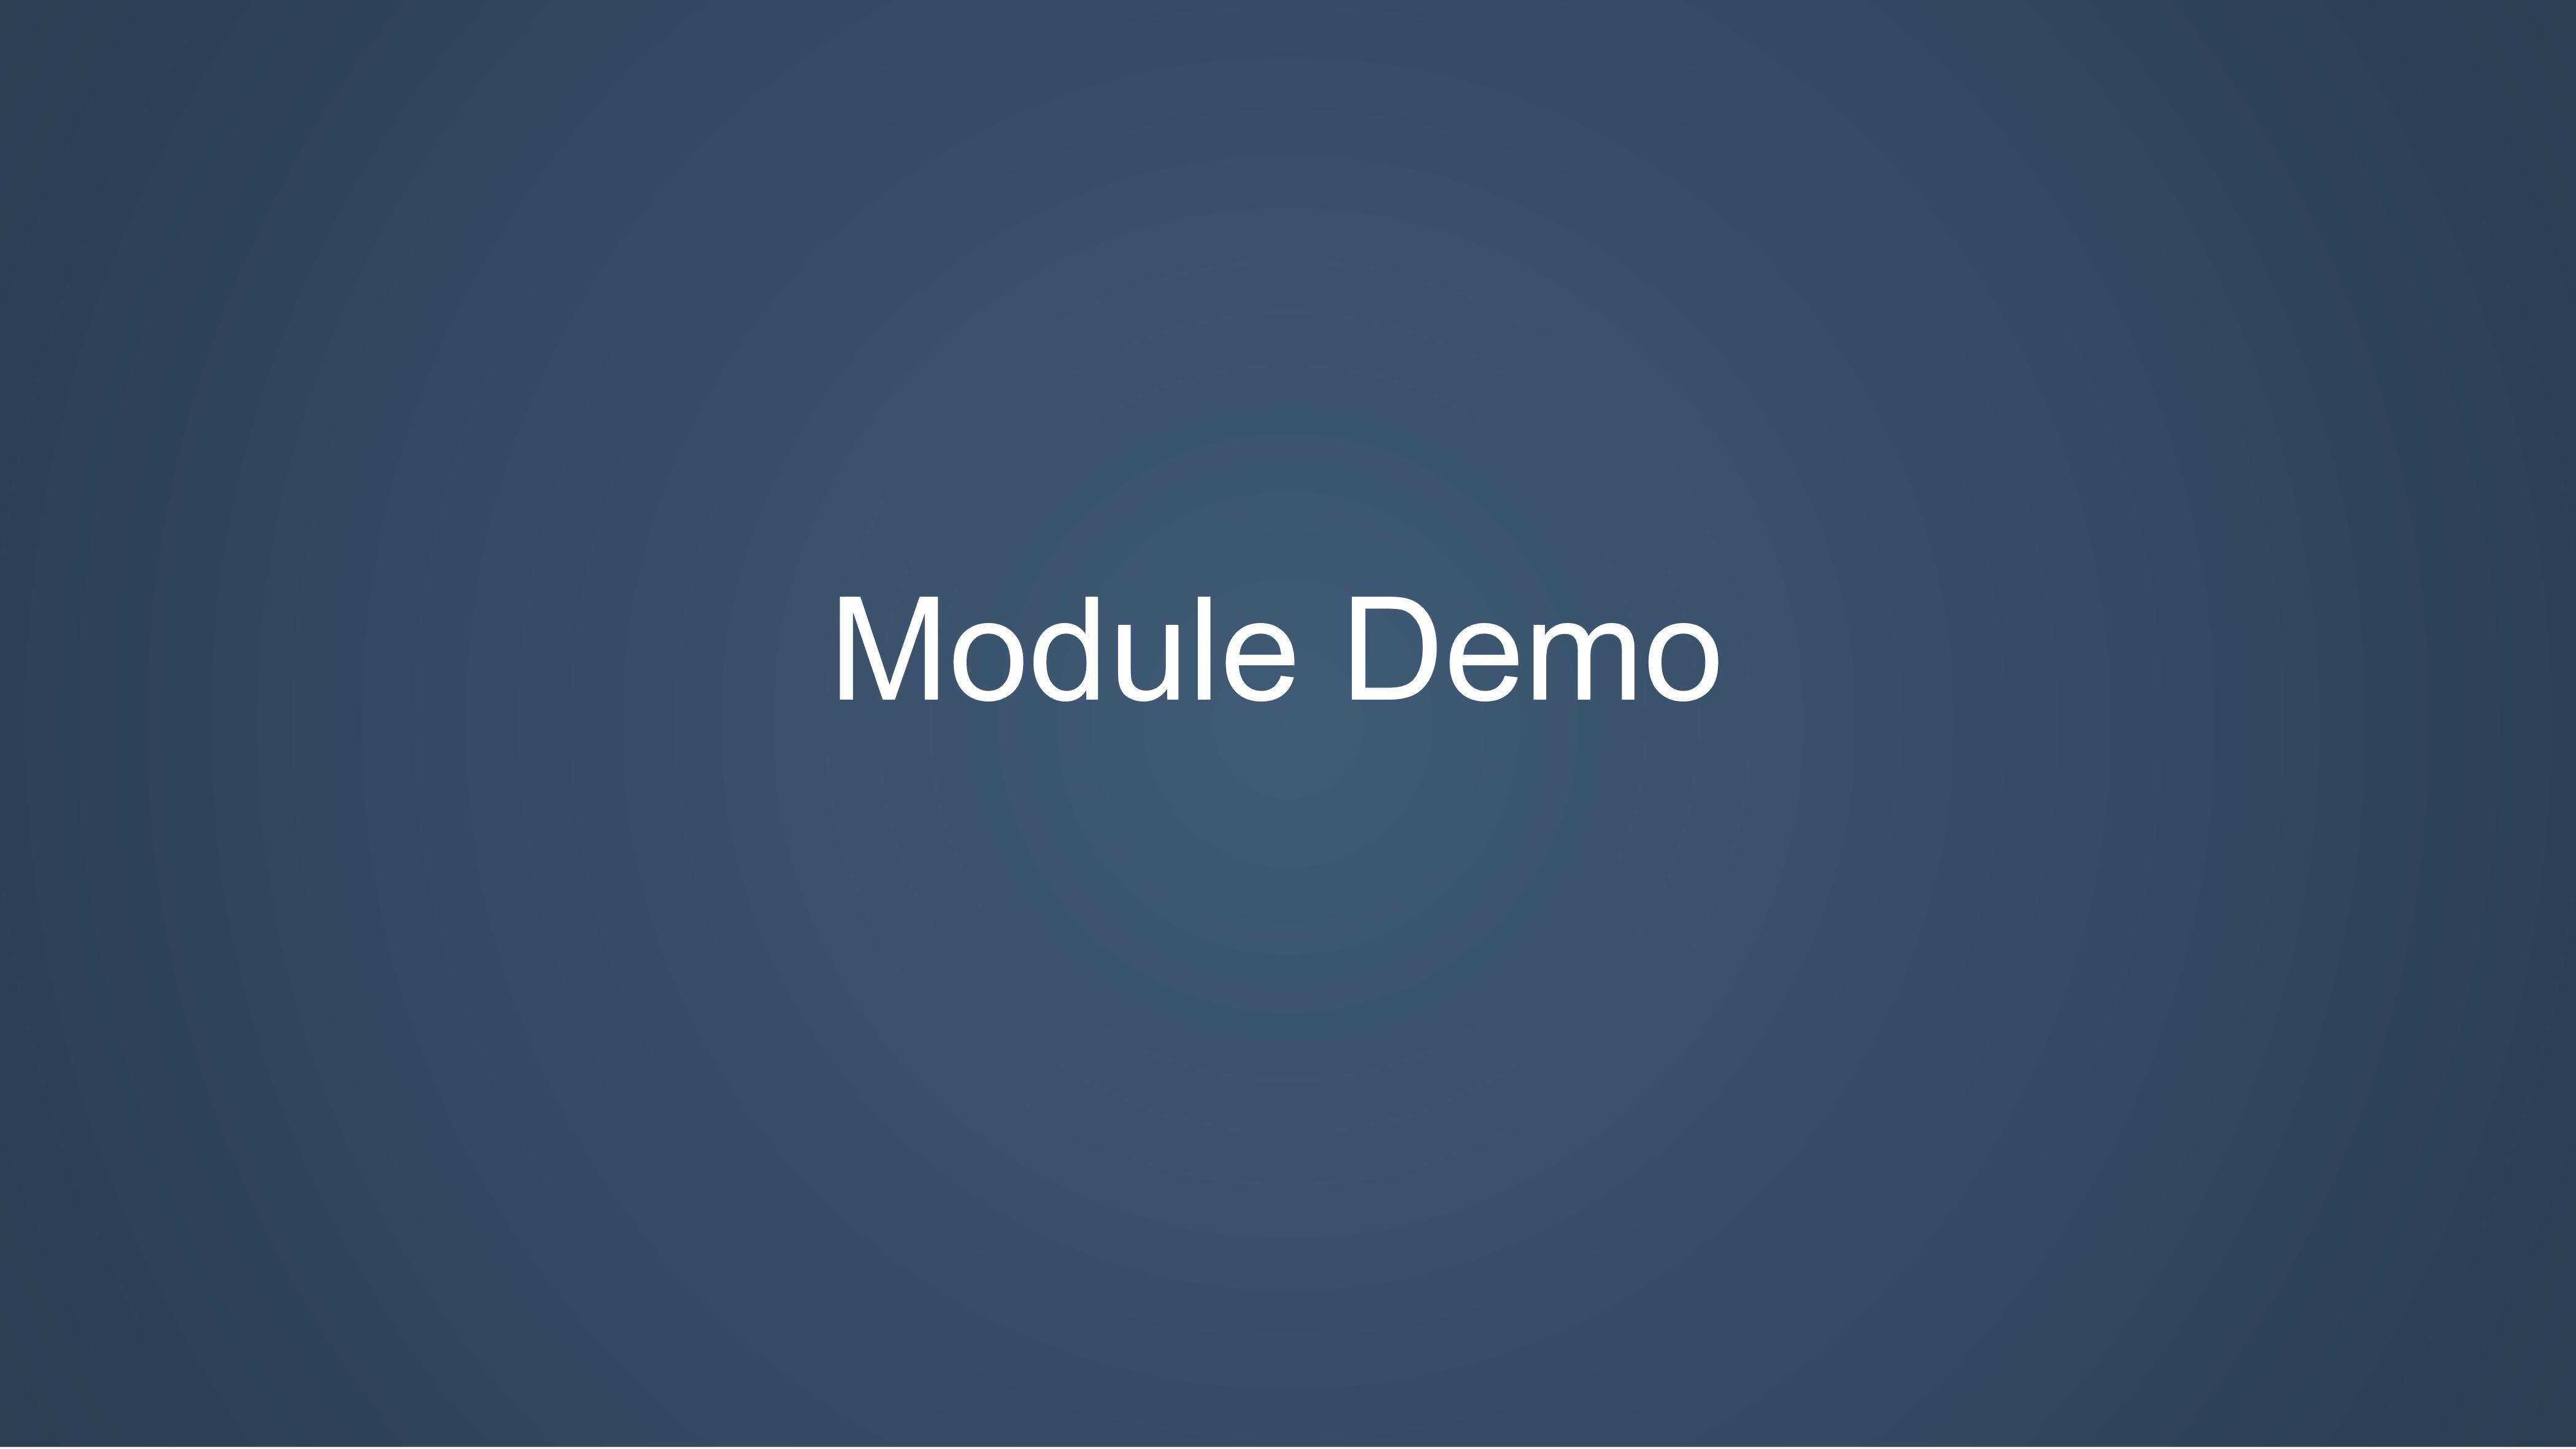
\includegraphics[scale=0.3]{0003.jpg}\vfill
		%\newline
		%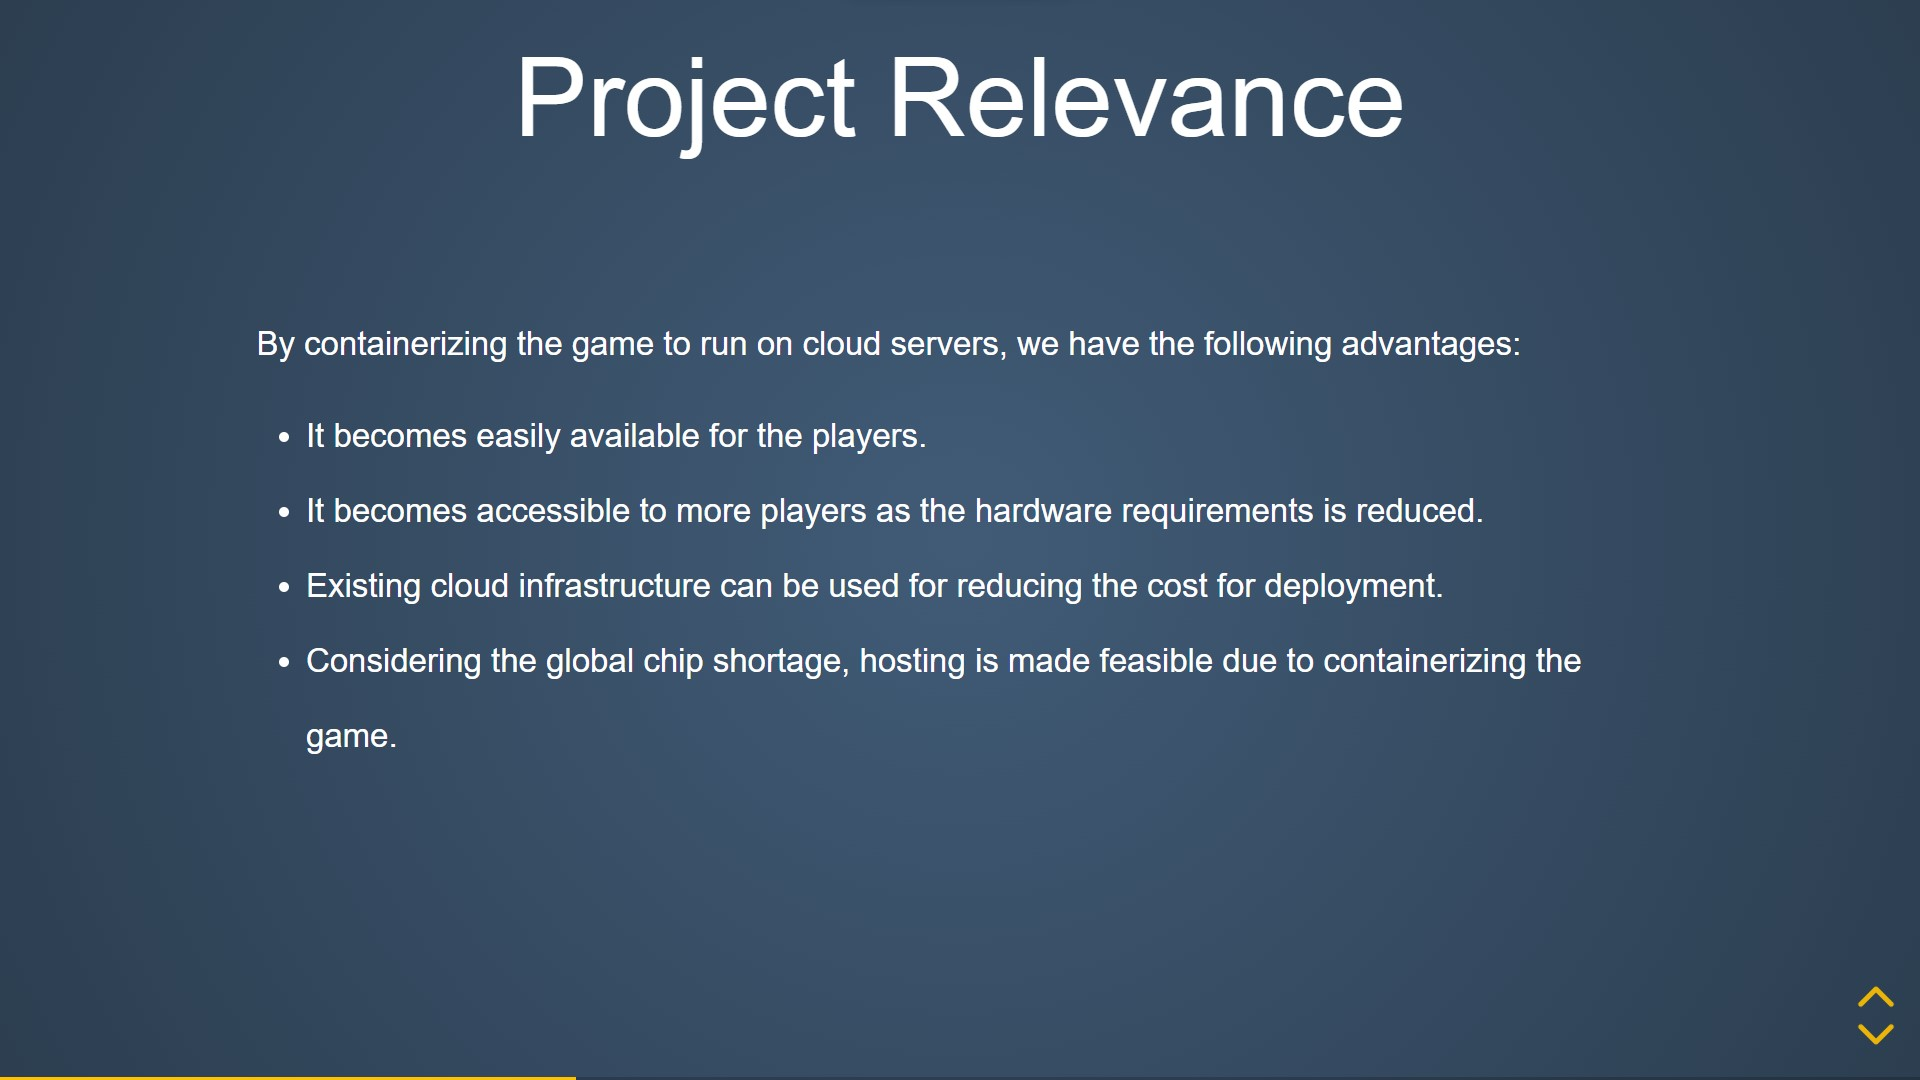
\includegraphics[scale=0.16]{s4.jpg}
	\end{figure}
	\pagebreak
	\begin{figure}[ht!]
		\centering
		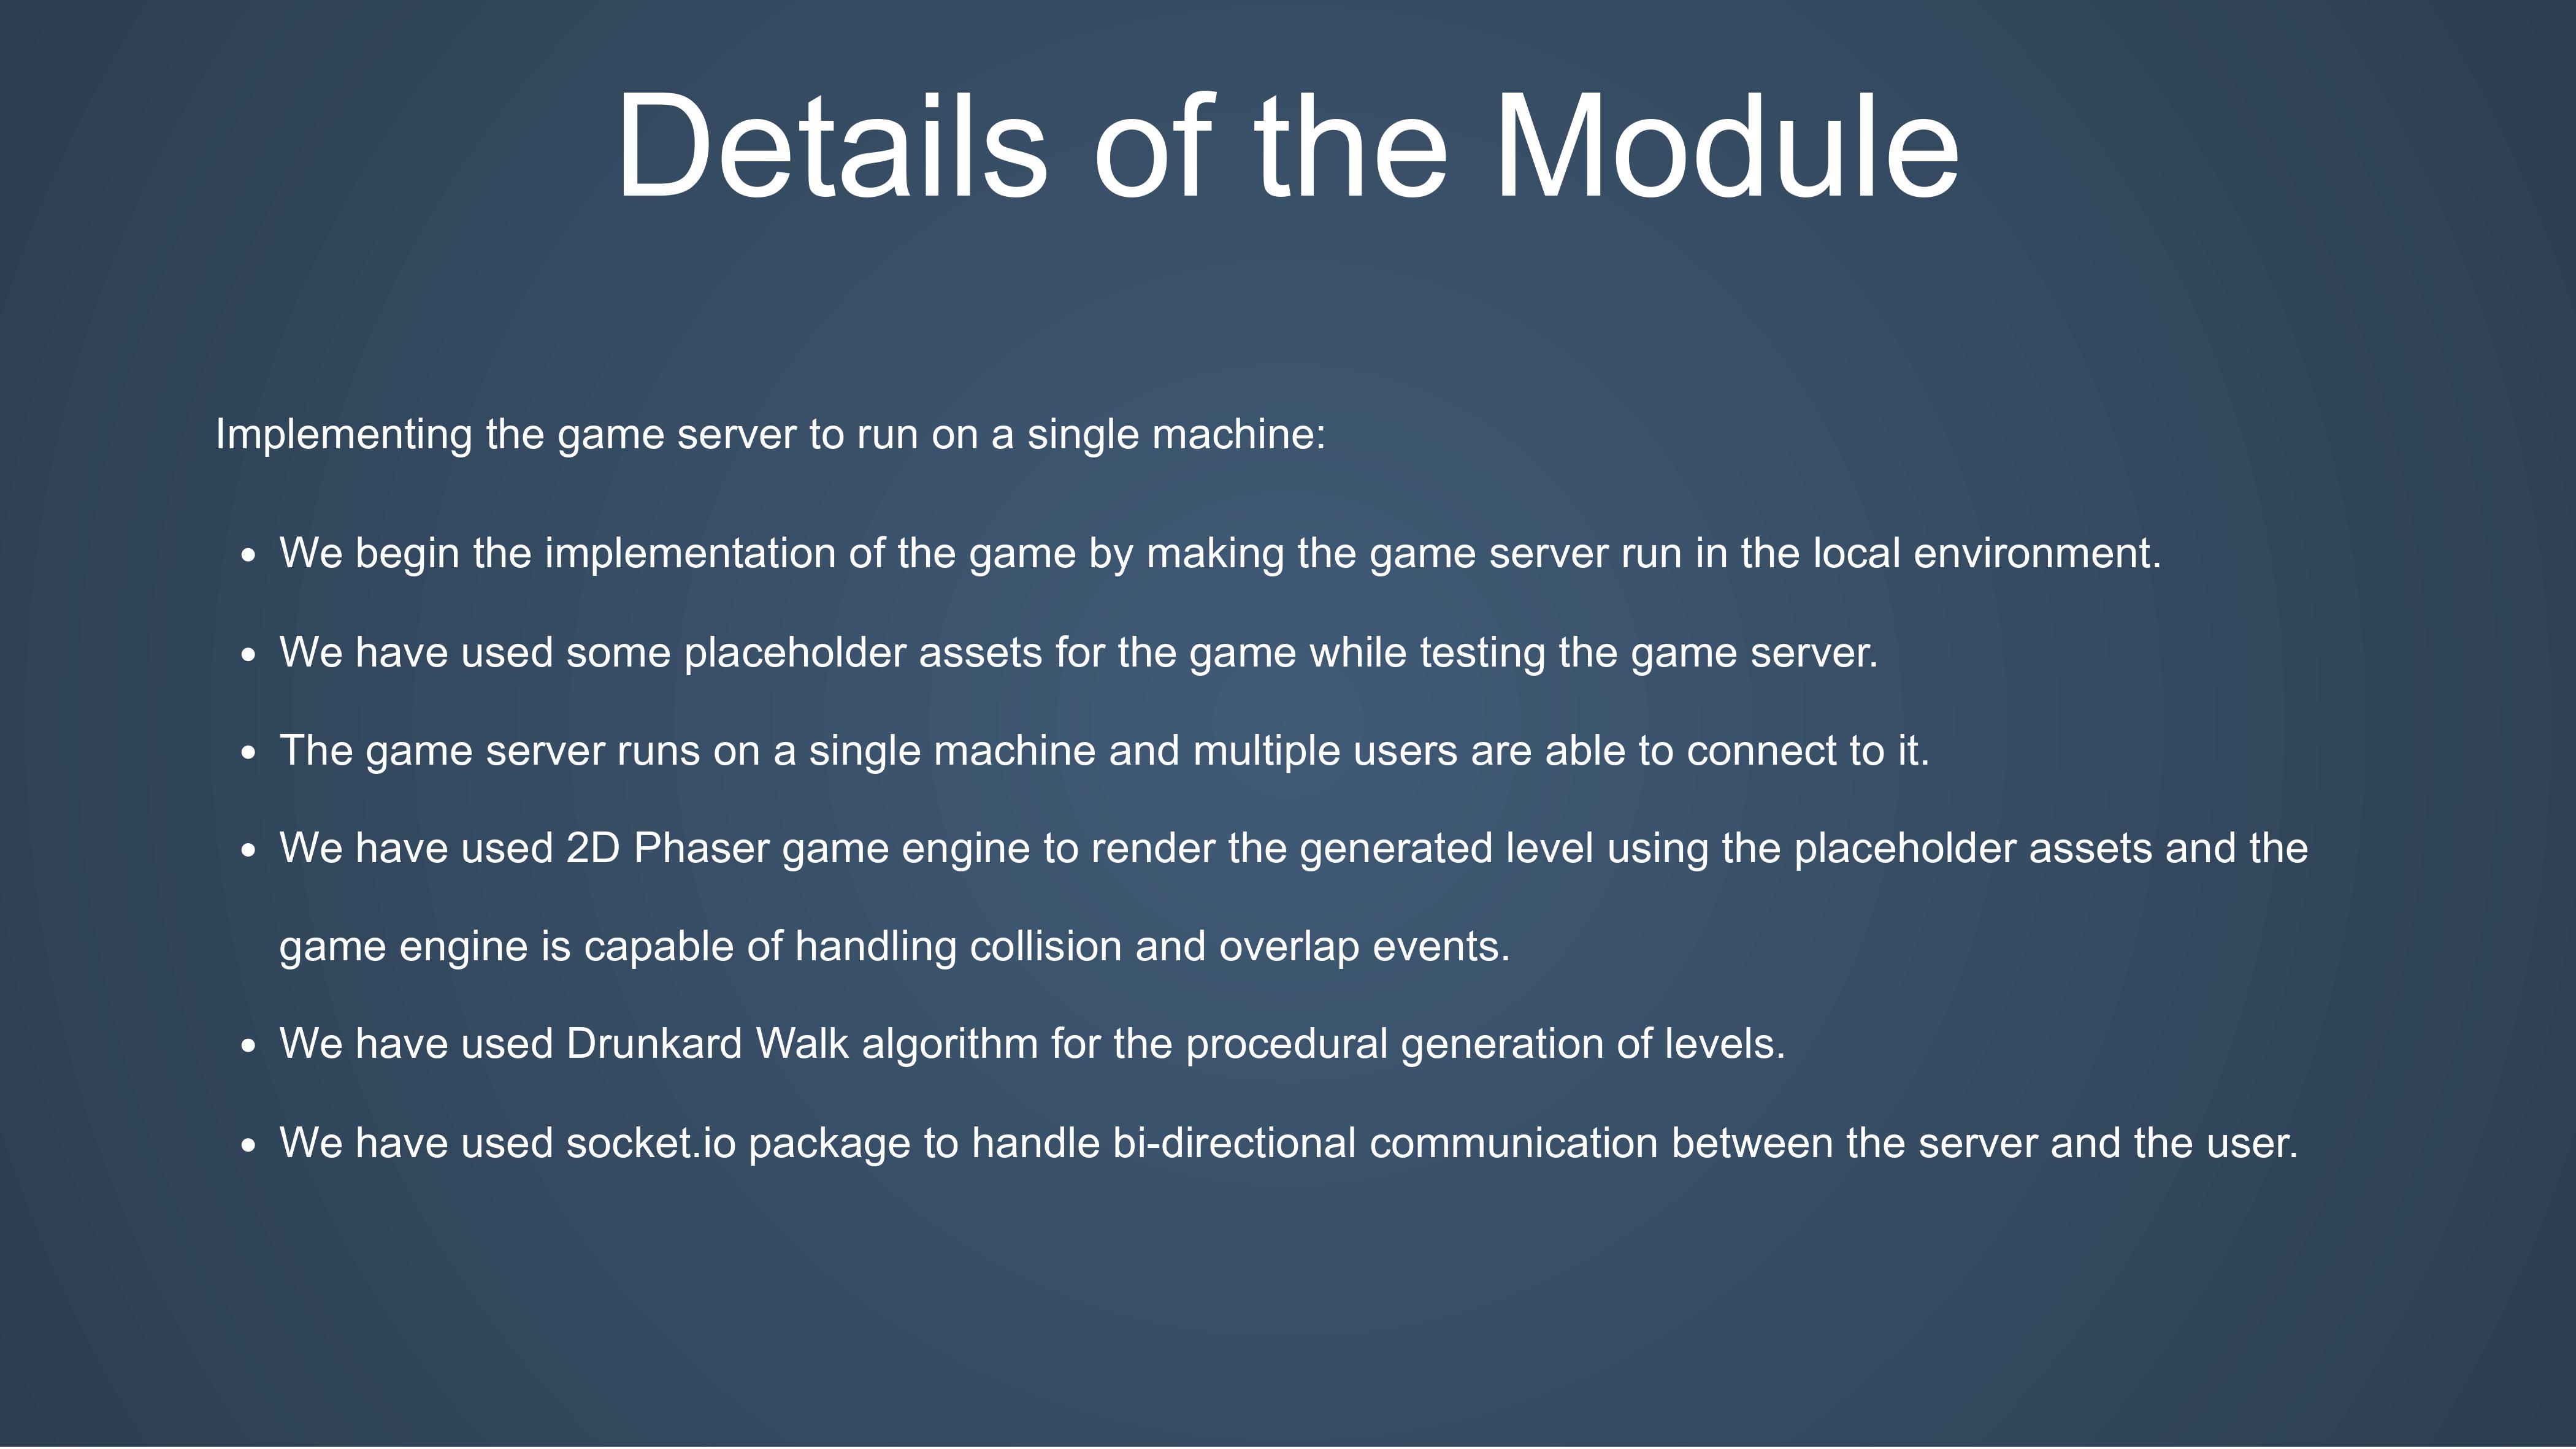
\includegraphics[scale=0.3]{0004.jpg}\vfill
		%\newline
		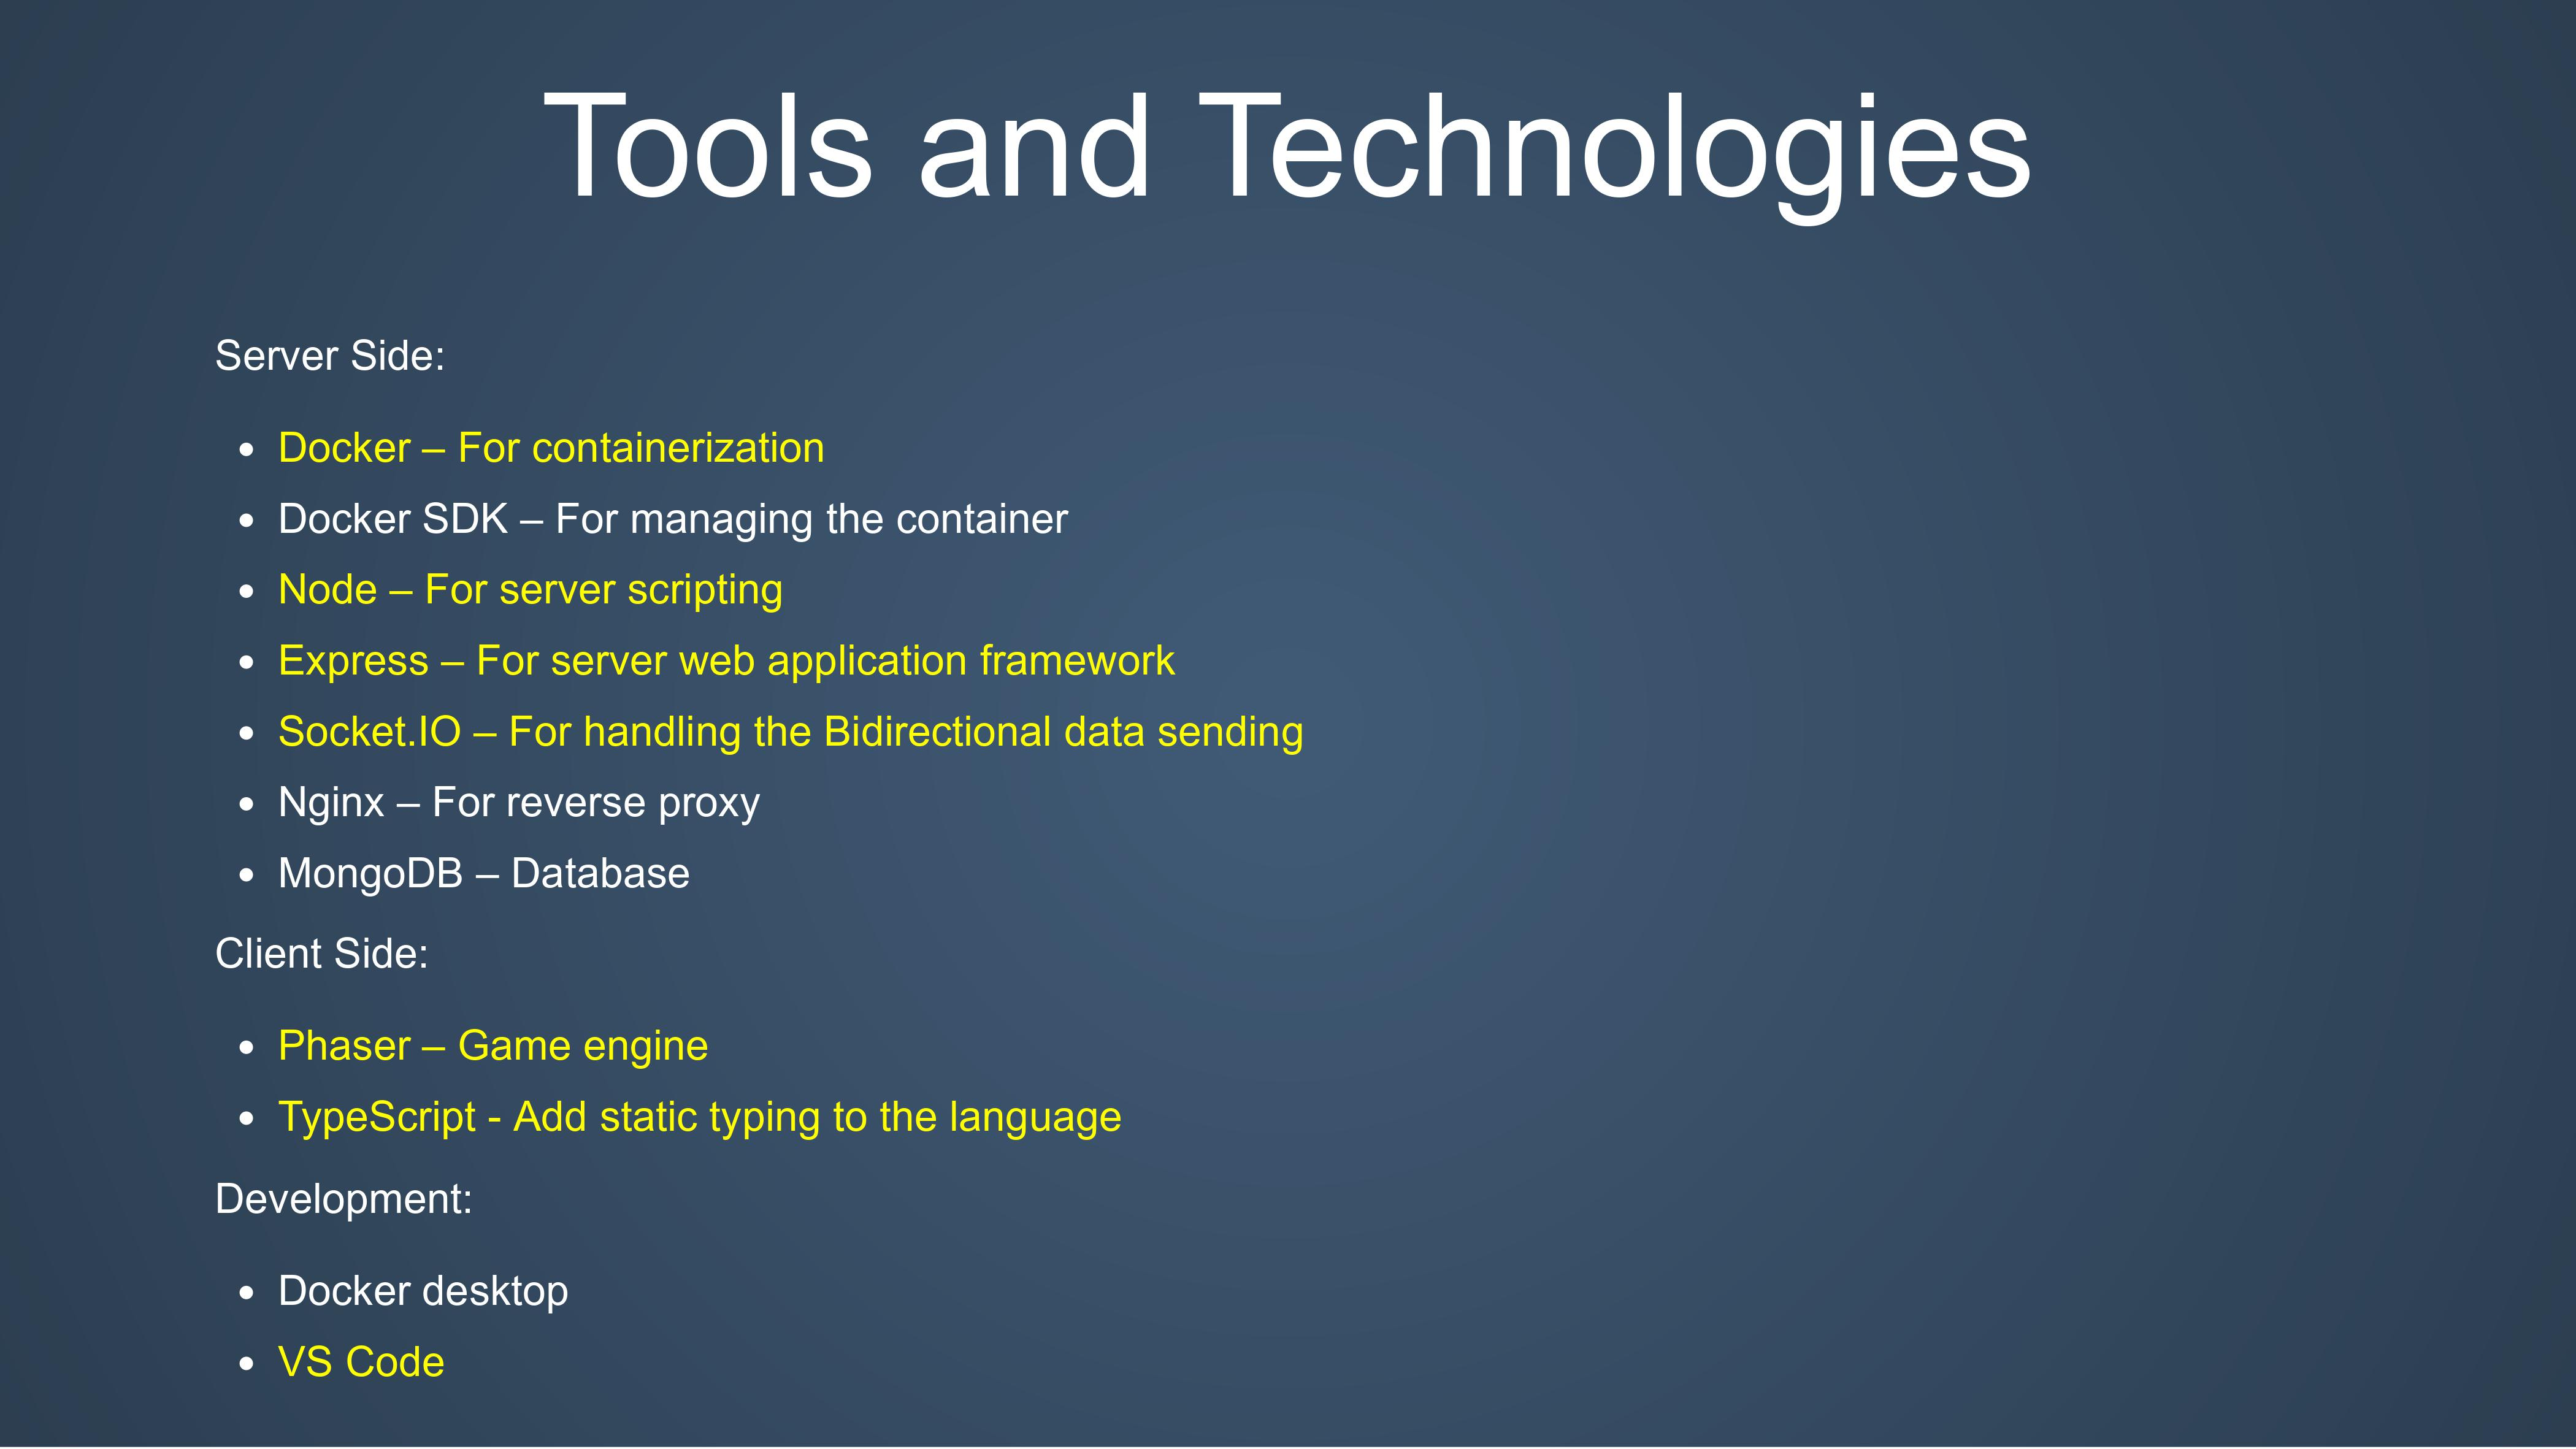
\includegraphics[scale=0.3]{0005.jpg}\vfill
		%\newline
		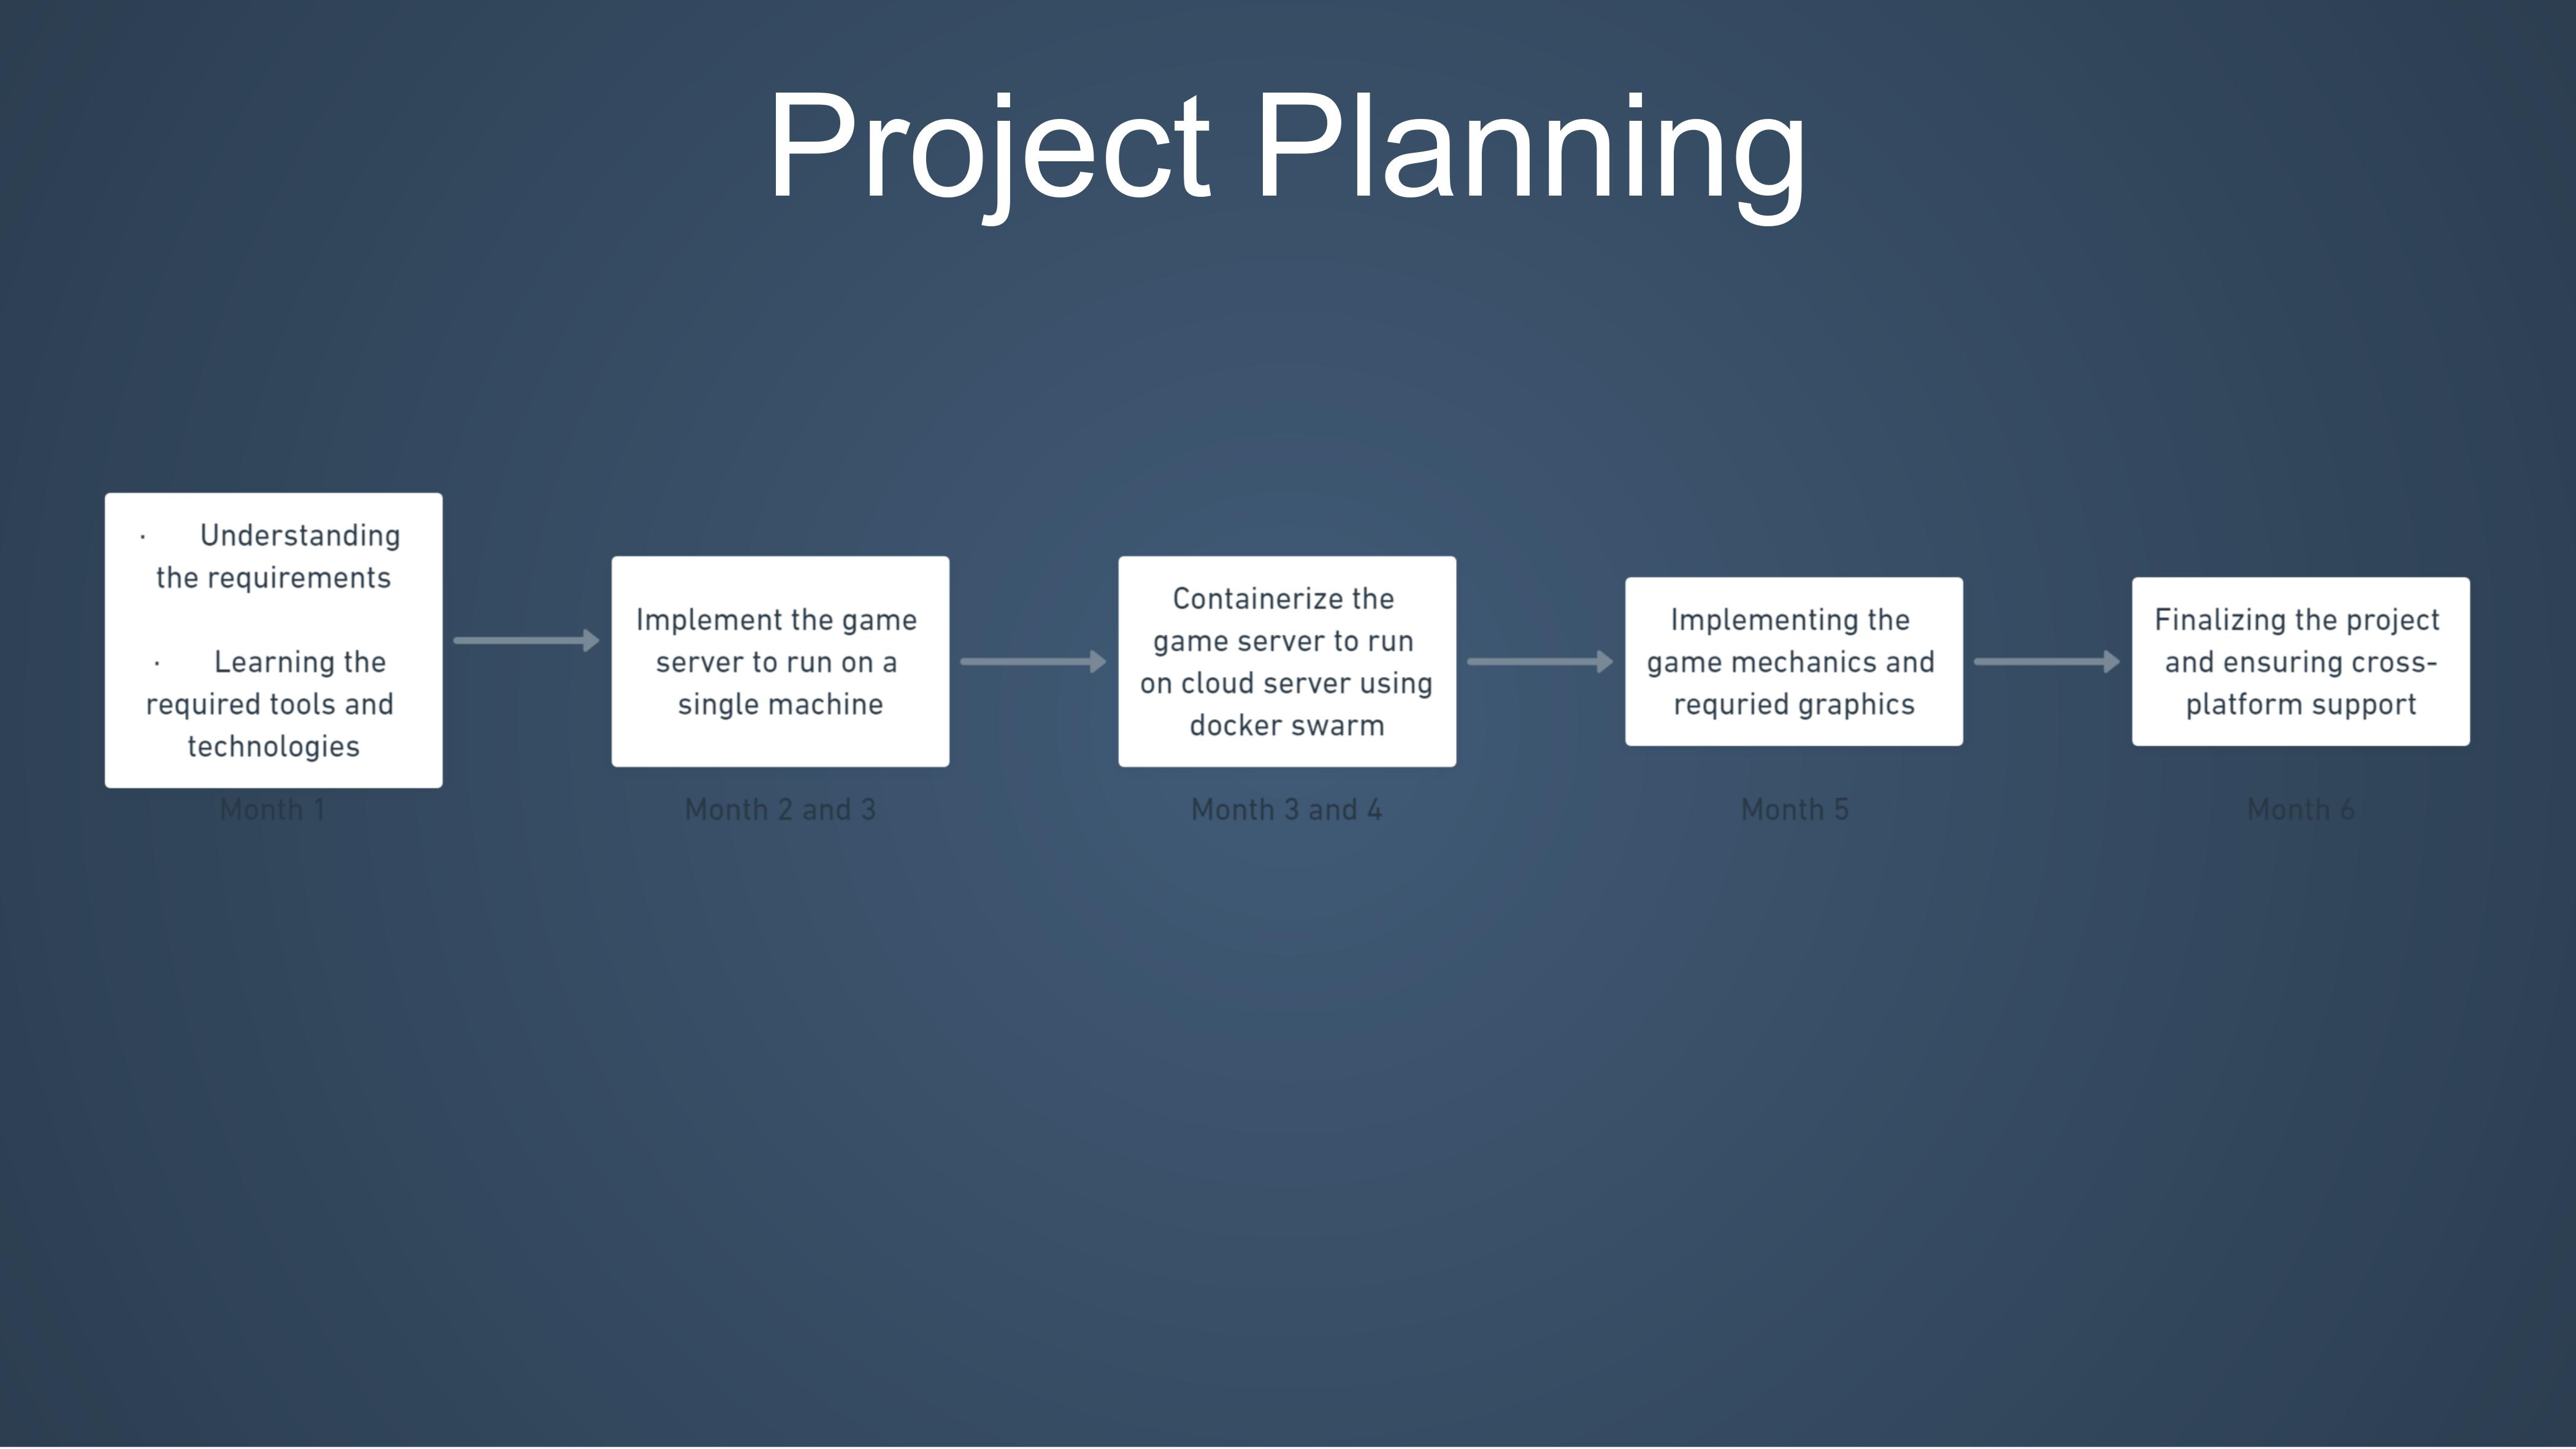
\includegraphics[scale=0.3]{0006.jpg}\vfill
		%\newline
		%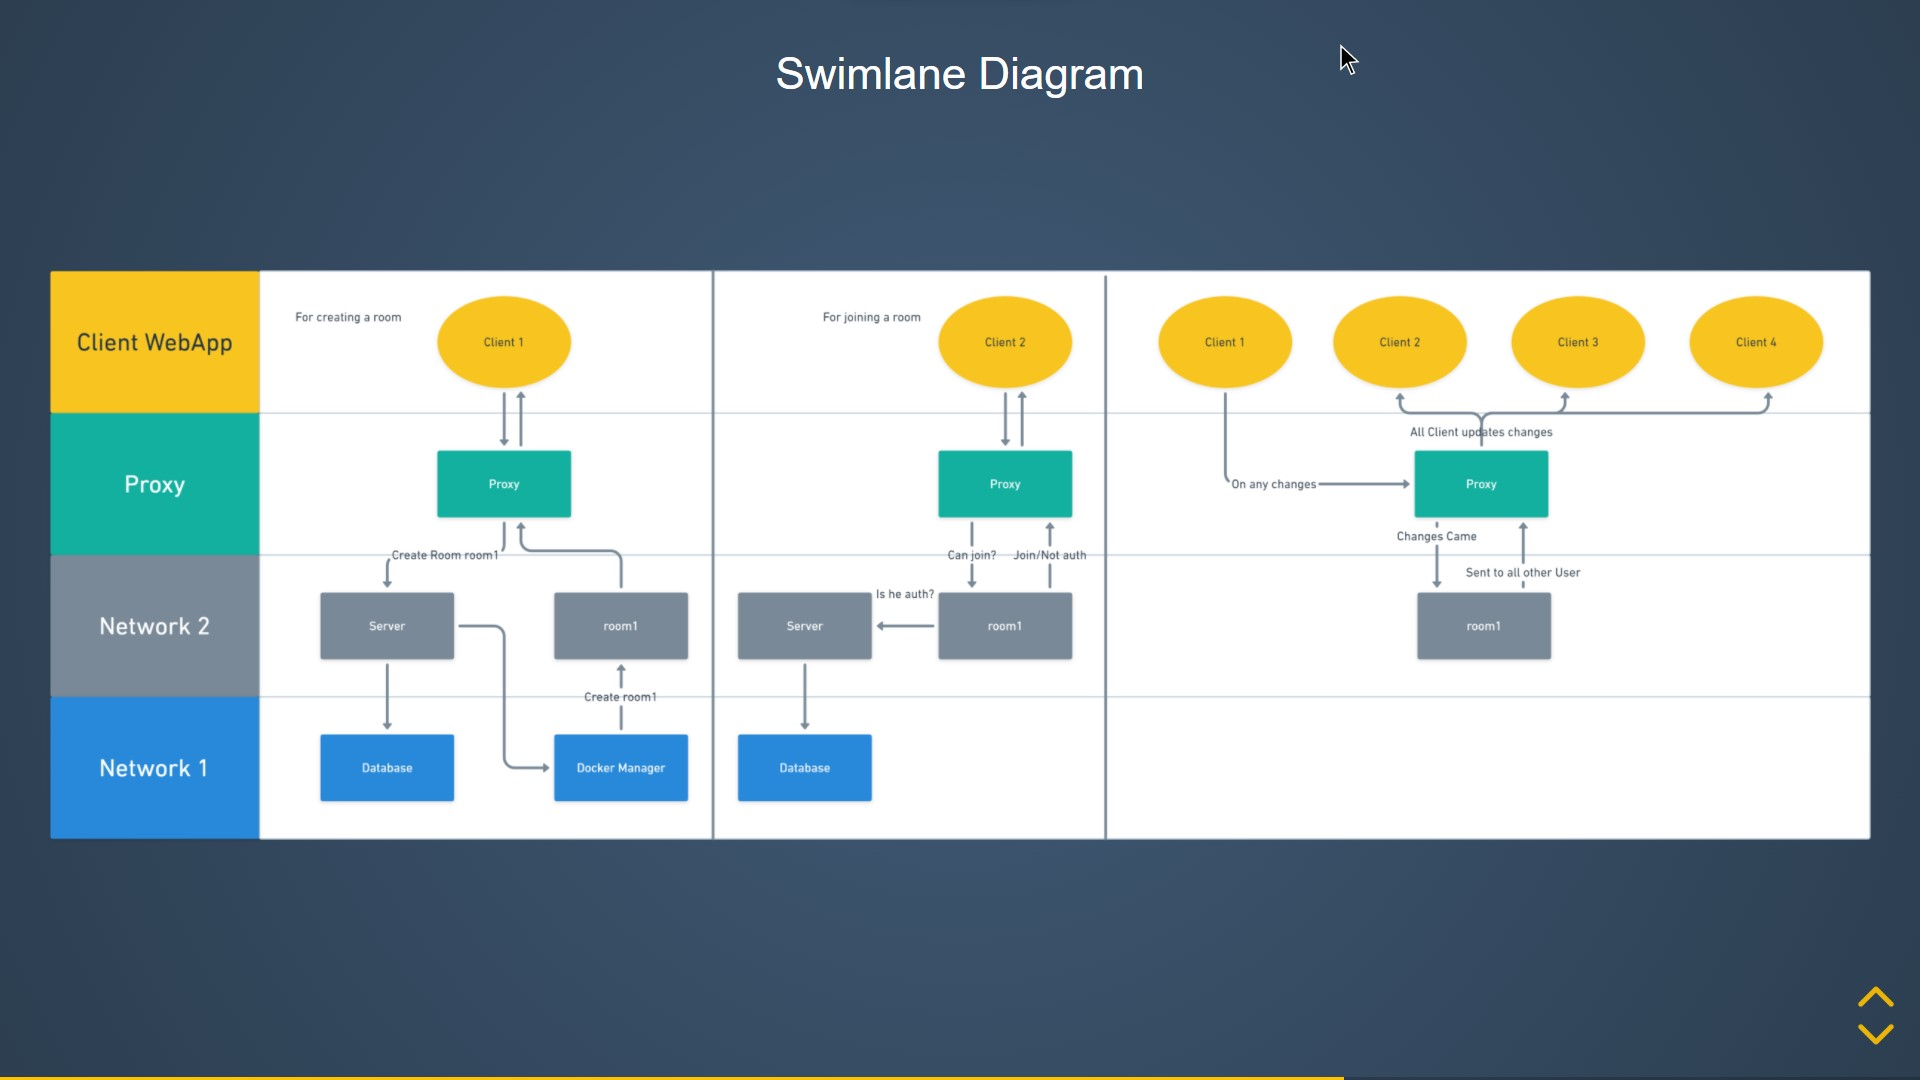
\includegraphics[scale=0.16]{s8.jpg}
	\end{figure}
	\pagebreak
	\begin{figure}[ht!]
		\centering
		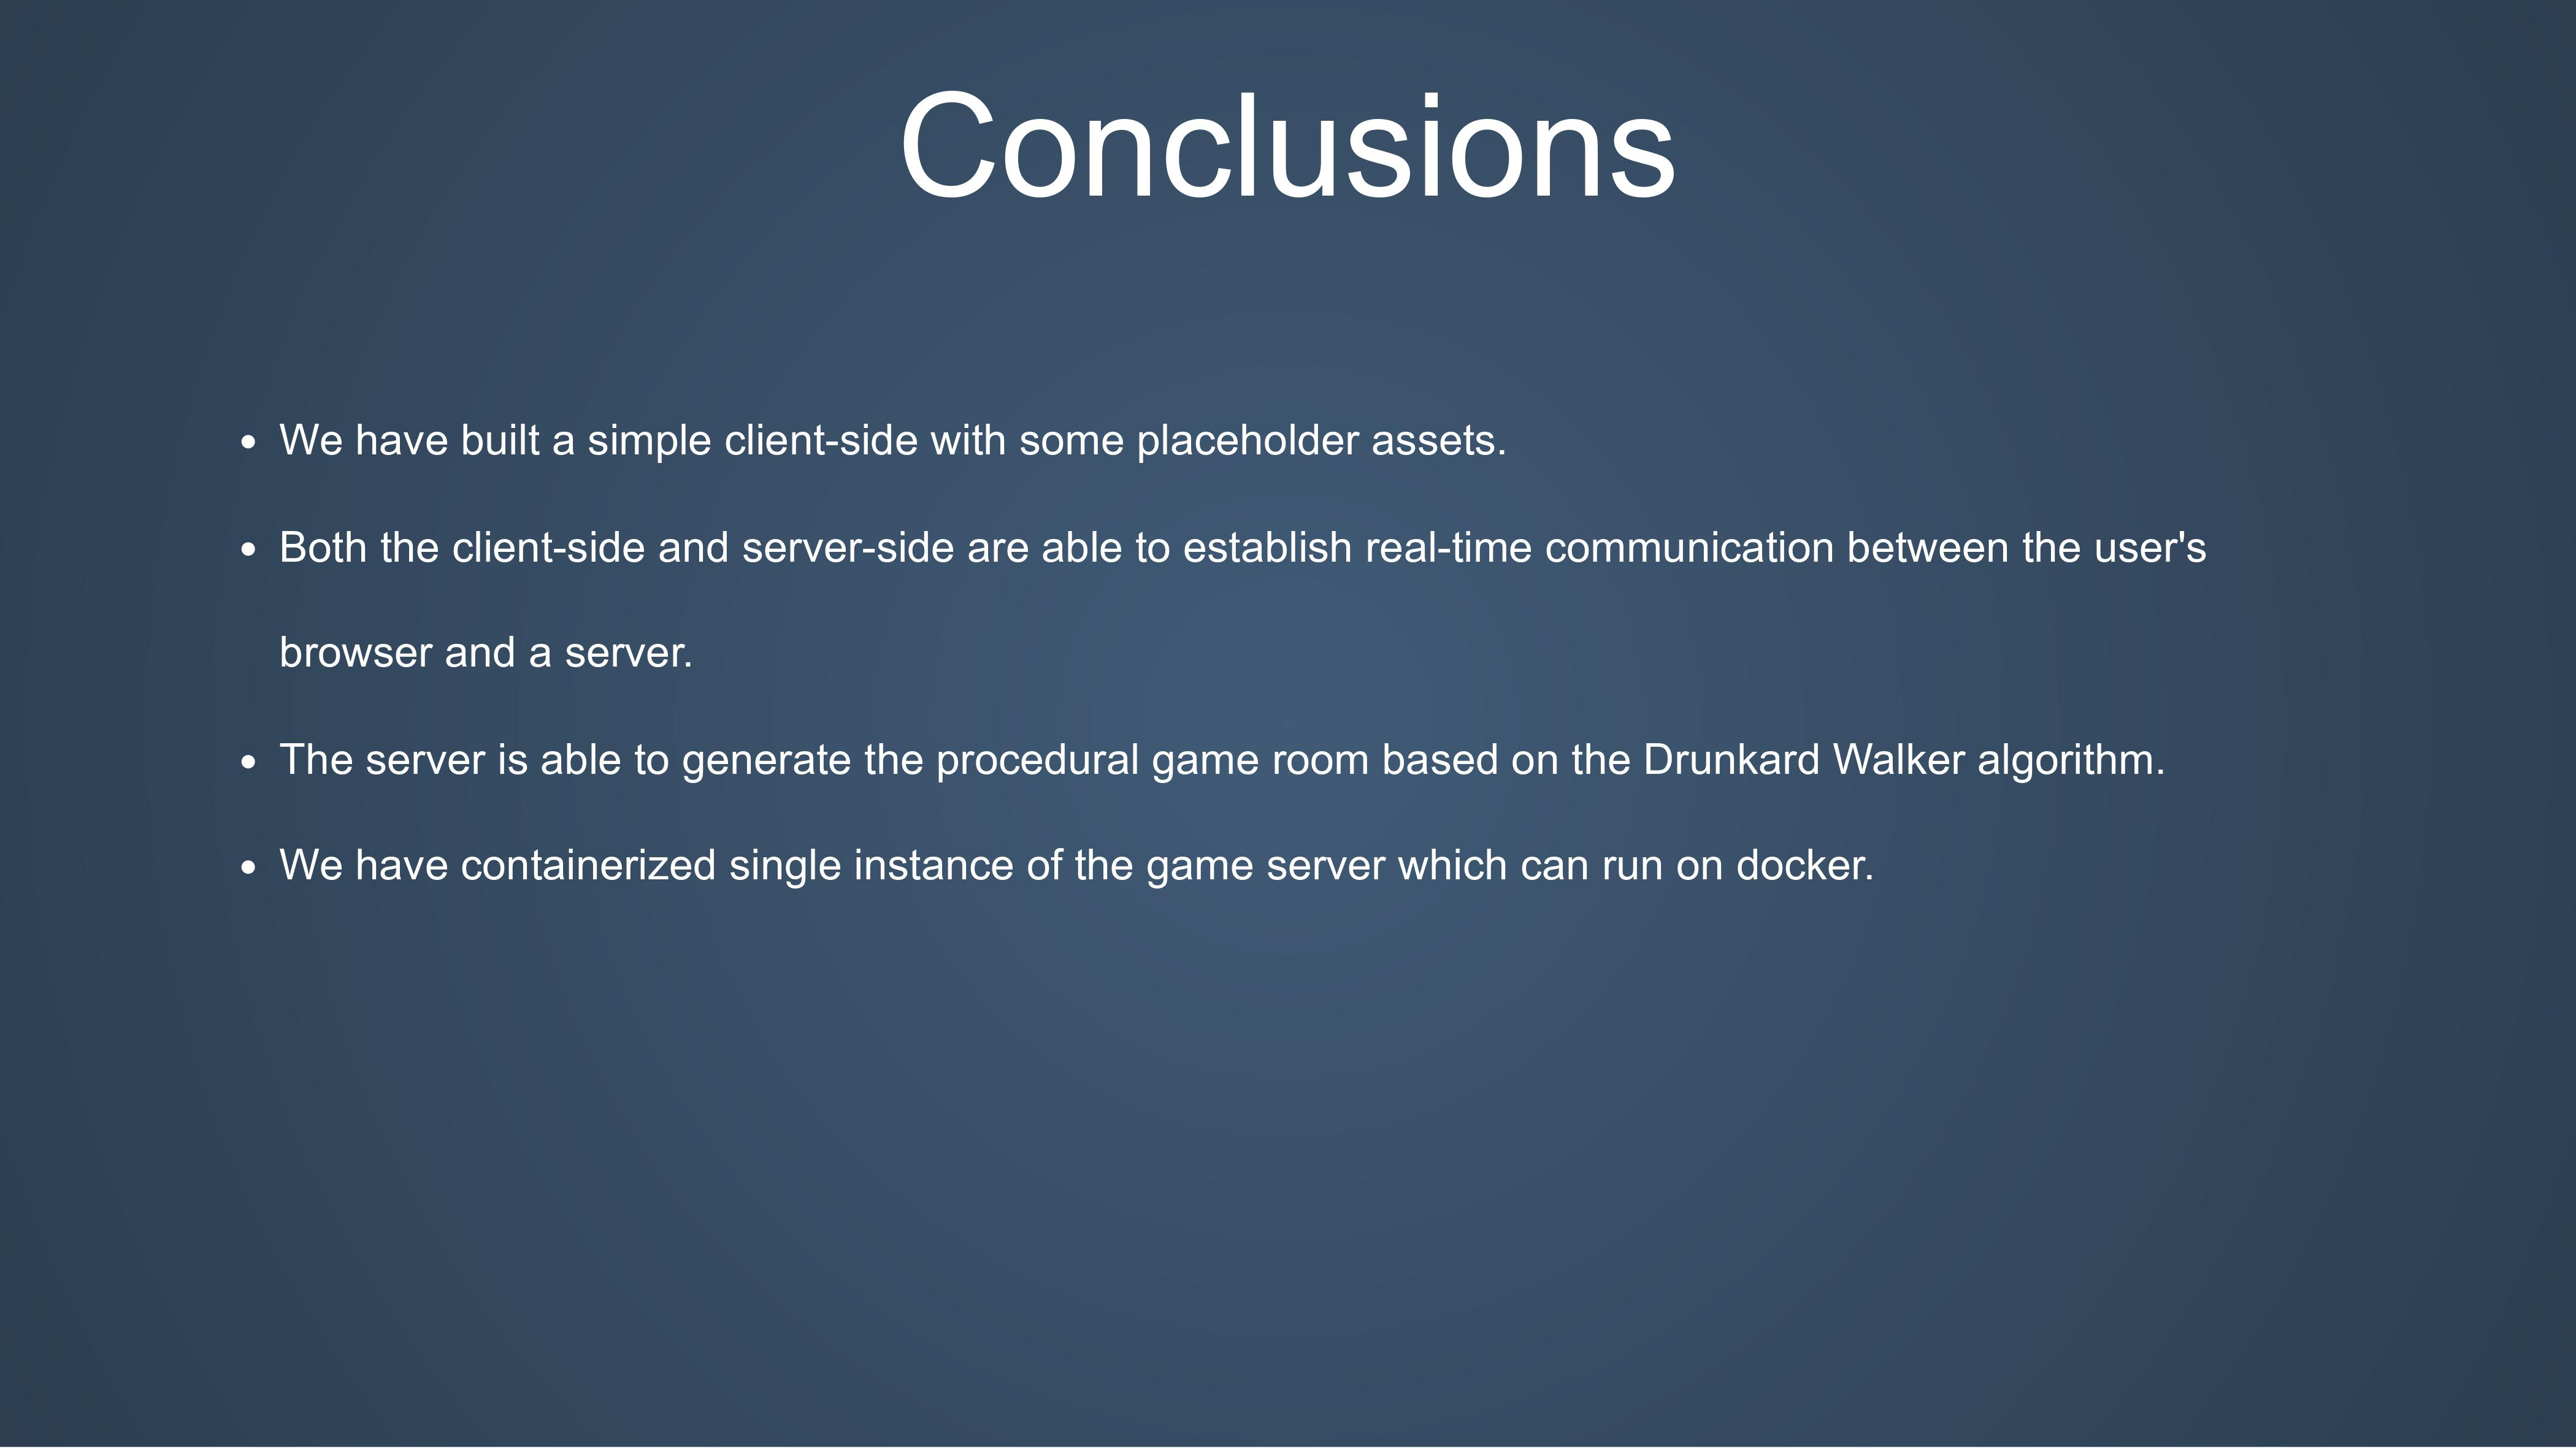
\includegraphics[scale=0.3]{0007.jpg}
		%\newline
		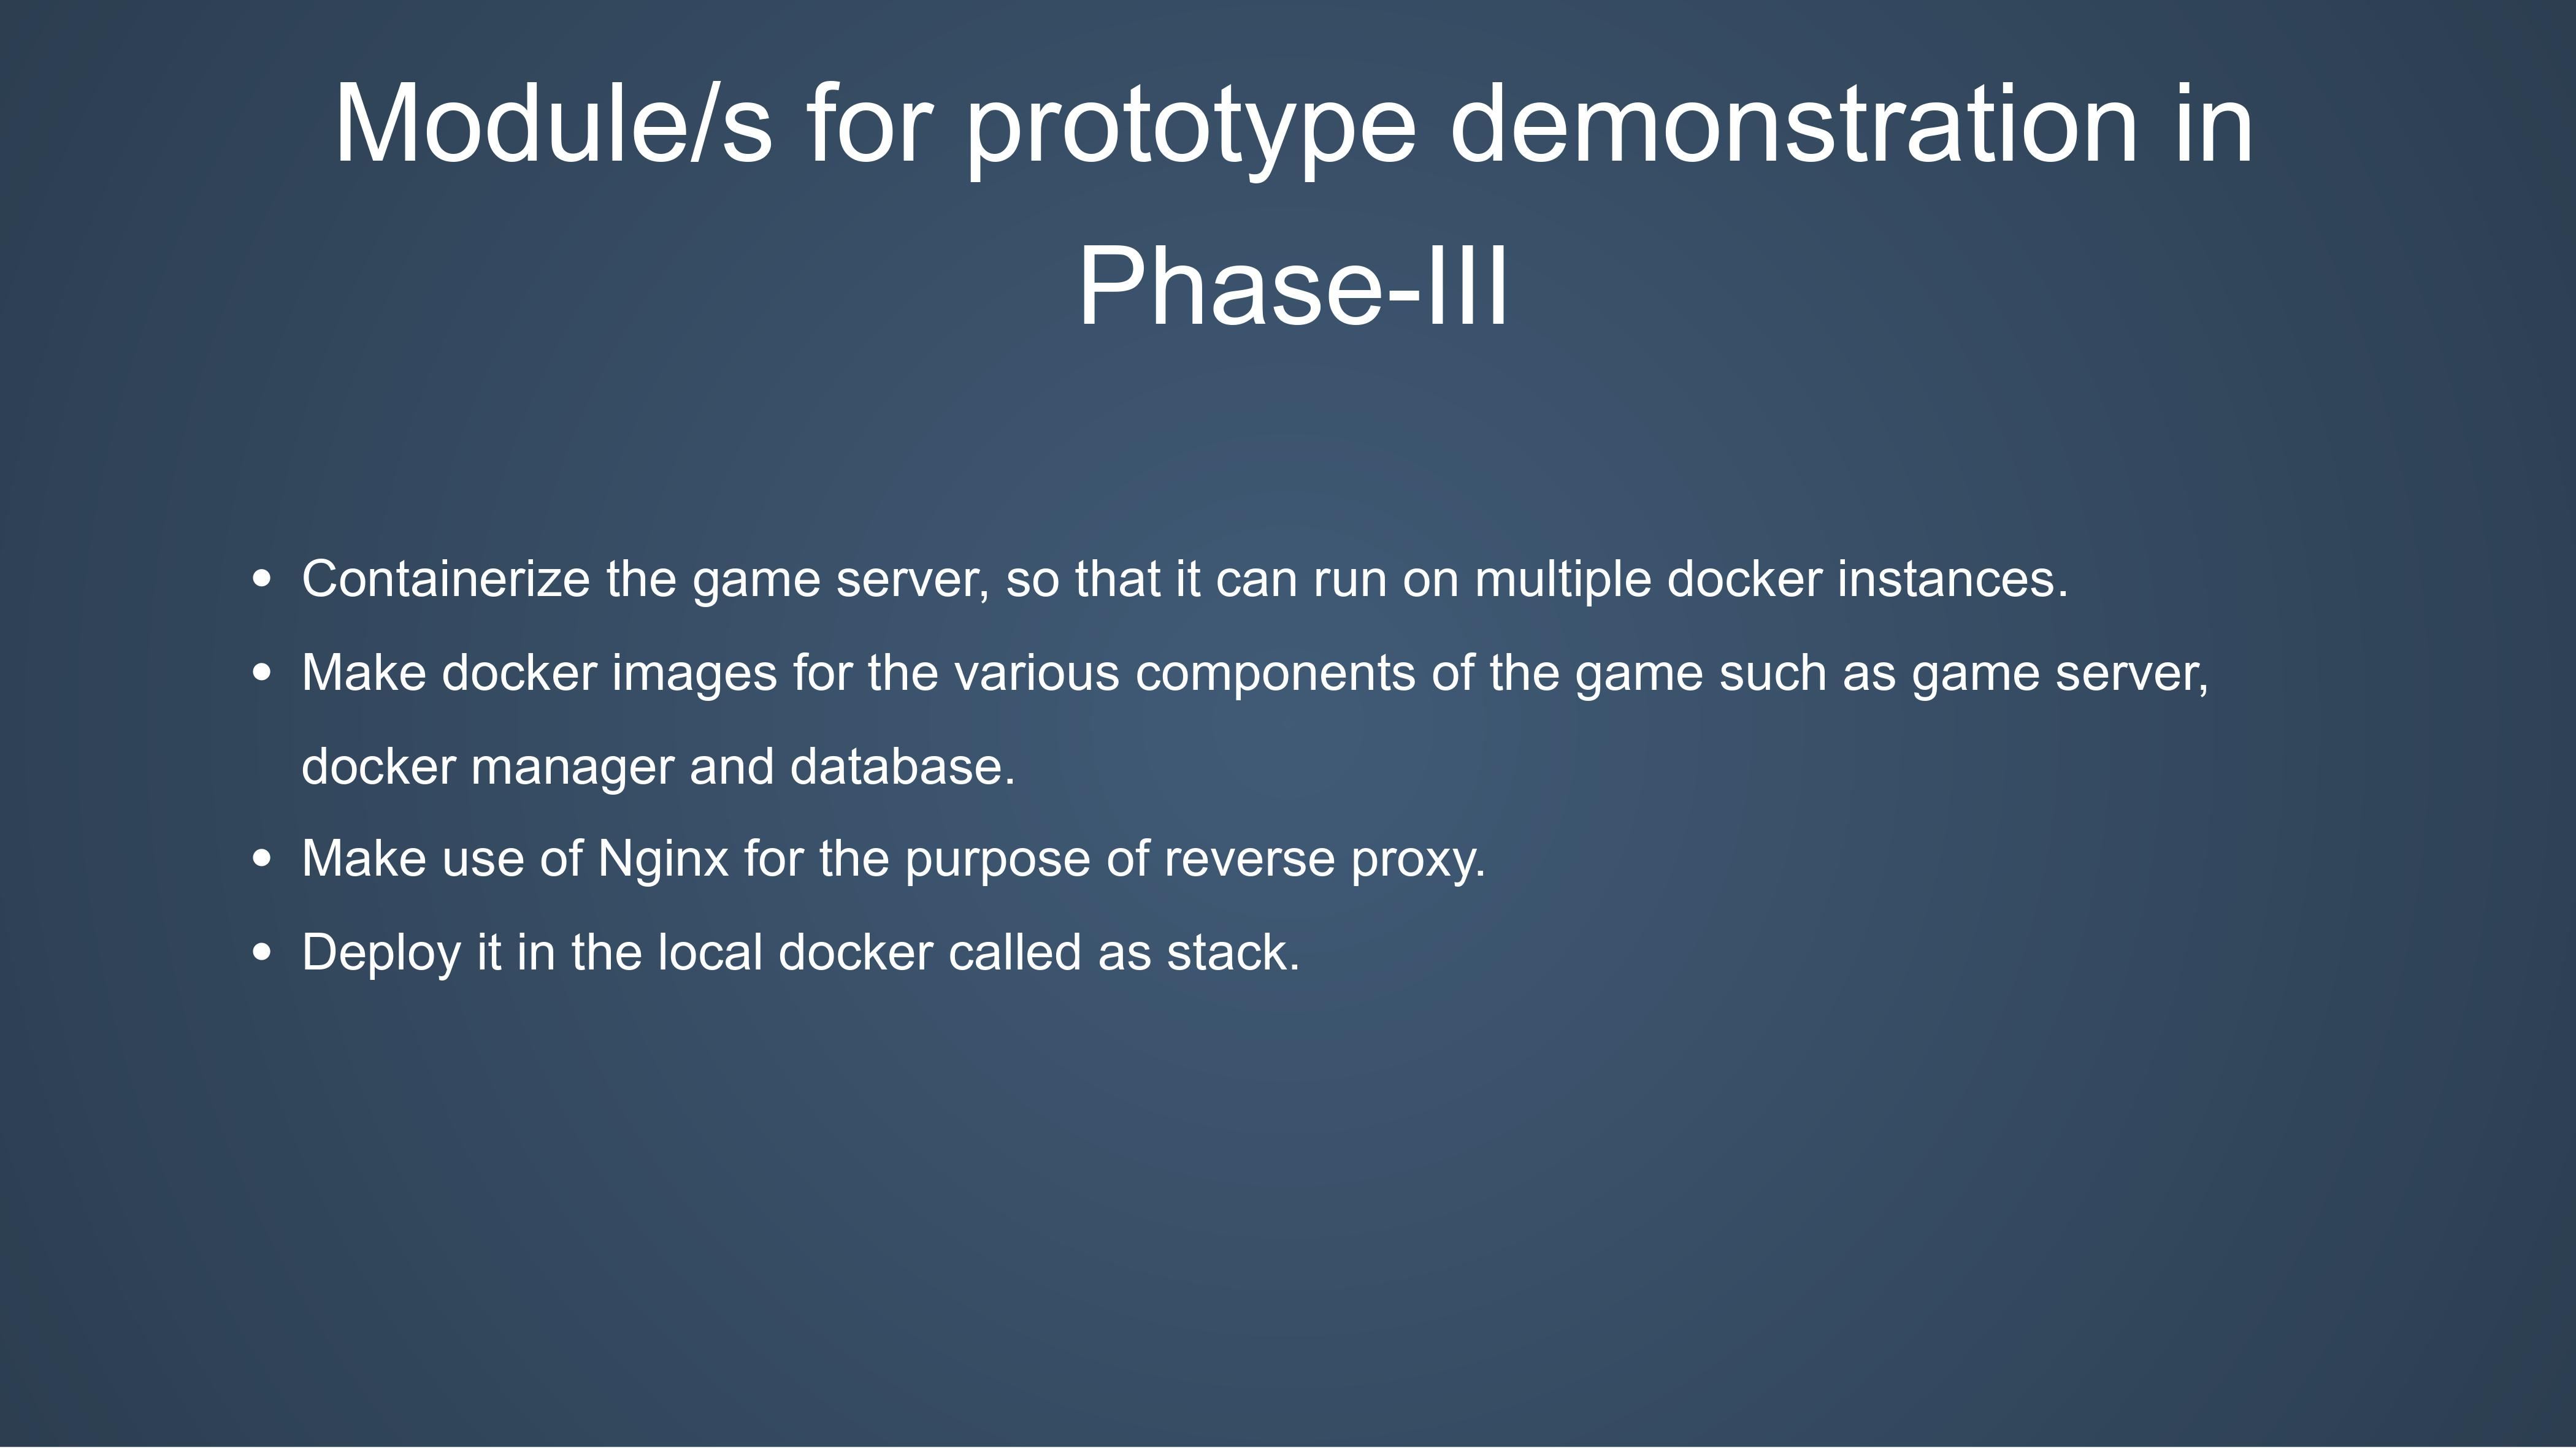
\includegraphics[scale=0.3]{0008.jpg}
		%\newline
		
\includegraphics[scale=0.3]{0009.jpg}
		%\newline
	\end{figure}
	\pagebreak	
	\pagebreak
	
	
\end{document}